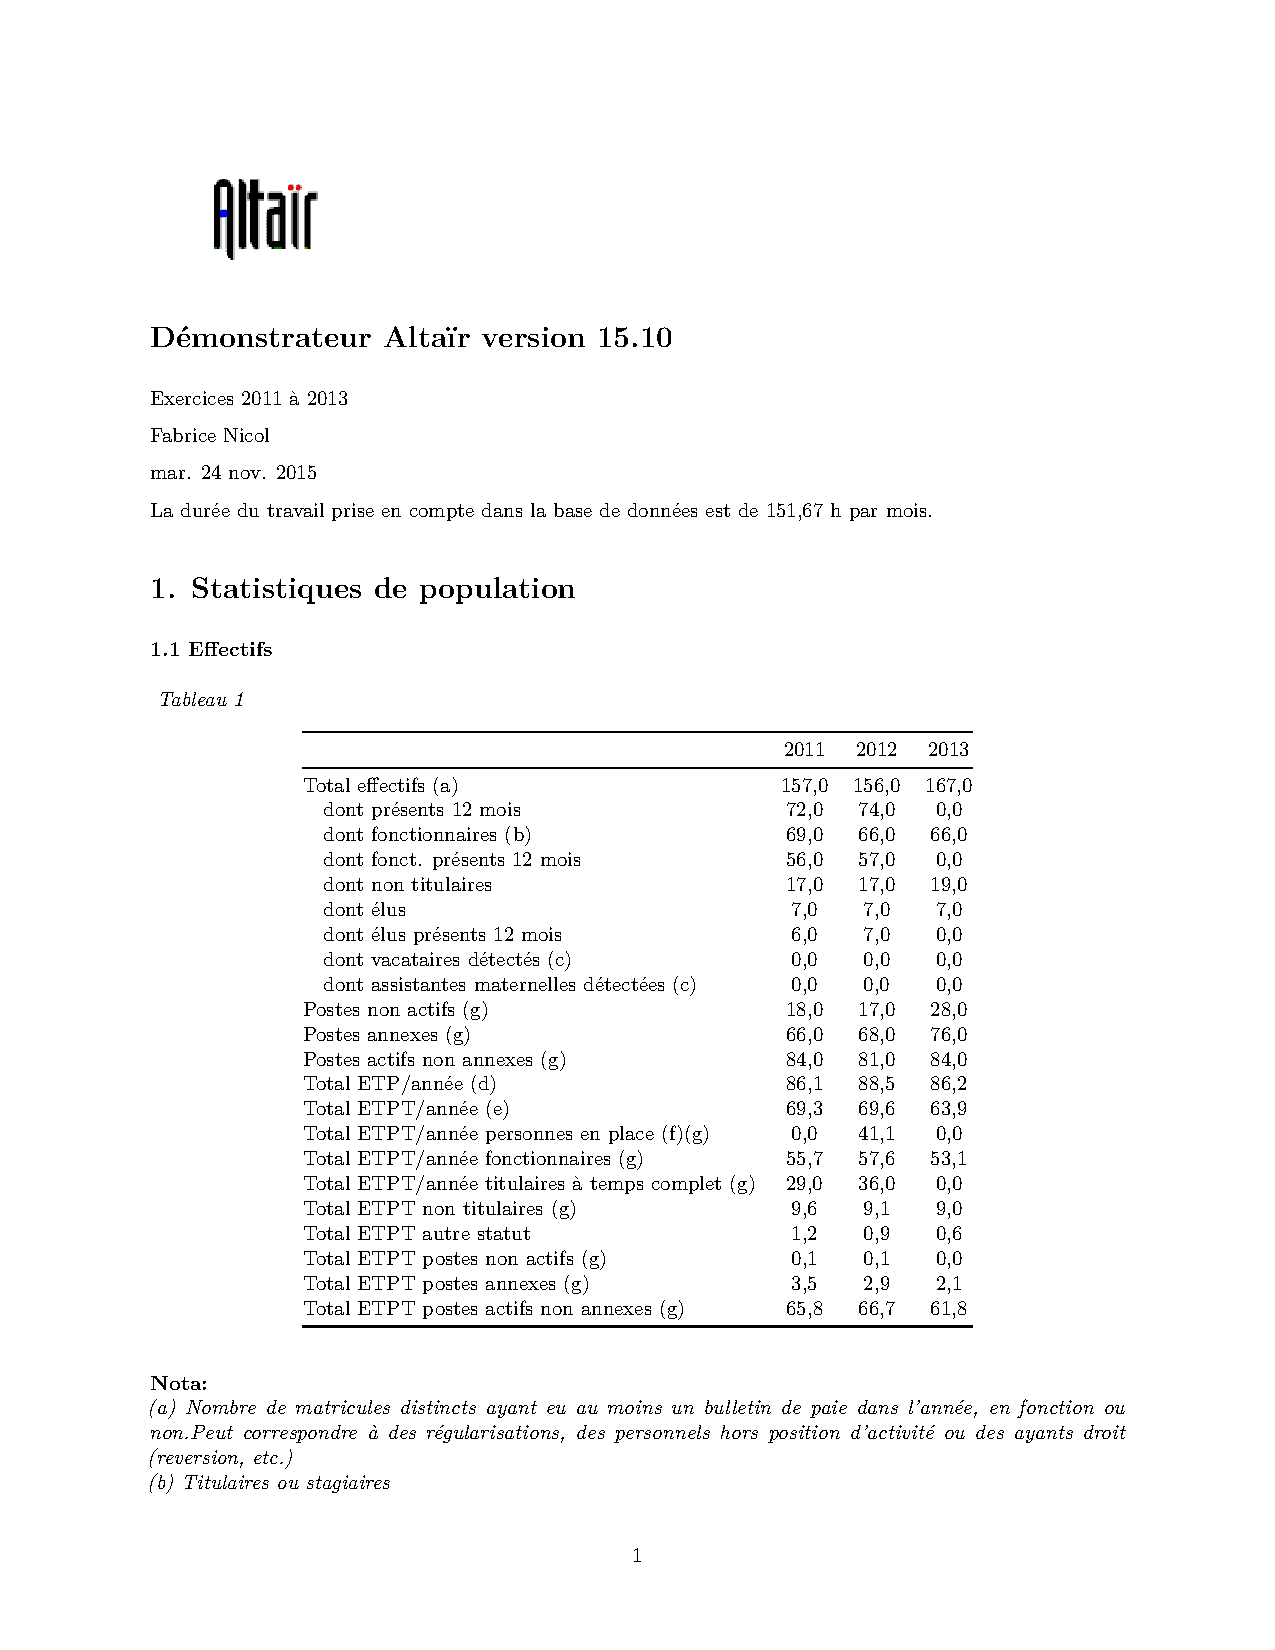
\includegraphics{icones/altair.png}

\hypertarget{logiciel-altair-version-20.08-5-ubuntu}{%
\subsection{Logiciel Altaïr version
20.08-5-Ubuntu}\label{logiciel-altair-version-20.08-5-ubuntu}}

\hypertarget{employeur-mairie-amplepuis}{%
\subsubsection{Employeur : MAIRIE
AMPLEPUIS}\label{employeur-mairie-amplepuis}}

\hypertarget{siret-21690006800018}{%
\subsubsection{Siret : 21690006800018}\label{siret-21690006800018}}

\hypertarget{etablissement-mairie-d}{%
\subsubsection{Etablissement : MAIRIE D}\label{etablissement-mairie-d}}

\hypertarget{budget-budget-ample-com-multi-budgets}{%
\subsubsection{Budget : Budget AMPLE COM, Multi
budgets}\label{budget-budget-ample-com-multi-budgets}}

\textbf{Période sous revue : 2009 - 2013 }\\
\textbf{Nombre d'exercices : 5 }

Logiciel sous licence \href{../Docs/LICENCE.html}{CeCILL v.2.1}

dim. 16 août 2020

\textbf{Avertissements}

\emph{1. La production des rapports d'analyse nécessite que les données
de paye soient continues, autrement dit qu'il n'y ait pas d'année ou de
mois manquant dans la série de données disponibles. Lorsque tel est le
cas, il convient de réaliser autant de rapports partiels que de séries
partielles de données continues.}

\emph{2. Il est recommandé de renseigner, dans toute la mesure du
possible, les codes de paye de l'onglet Codes de l'interface graphique}
~
\href{../Docs/Notices/fiche_onglet_codes.odt}{\includegraphics{icones/Notice.png}}

En cas de dysfonctionnement logiciel, veuillez bien signaler les
difficultés rencontrées au développeur.

\hypertarget{statistiques-de-population}{%
\section{1. Statistiques de
population}\label{statistiques-de-population}}

\hypertarget{effectifs}{%
\subsection{1.1 Effectifs}\label{effectifs}}

~\emph{Tableau 1.1.1 : Effectifs}

\begin{longtable}[]{@{}lcccccc@{}}
\toprule
& Effectifs & 2009 & 2010 & 2011 & 2012 & 2013\tabularnewline
\midrule
\endhead
1 & Matricules gérés en base (a) & 114,0 & 93,0 & 102,0 & 80,0 &
97,0\tabularnewline
2 & ~~~dont présents 12 mois & 54,0 & 56,0 & 55,0 & 57,0 &
1,0\tabularnewline
3 & ~~~dont fonctionnaires (b) & 47,0 & 45,0 & 51,0 & 47,0 &
48,0\tabularnewline
4 & ~~~dont fonct. présents 12 mois & 45,0 & 45,0 & 45,0 & 45,0 &
0,0\tabularnewline
5 & ~~~dont non titulaires & 50,0 & 26,0 & 31,0 & 12,0 &
29,0\tabularnewline
6 & ~~~dont élus & 9,0 & 9,0 & 9,0 & 9,0 & 9,0\tabularnewline
7 & ~~~dont élus présents 12 mois & 7,0 & 9,0 & 9,0 & 9,0 &
0,0\tabularnewline
8 & ~~~dont vacataires détectés (c) & 0,0 & 0,0 & 0,0 & 0,0 &
0,0\tabularnewline
9 & ~~~dont assistantes maternelles détectées (c) & 0,0 & 0,0 & 0,0 &
0,0 & 0,0\tabularnewline
10 & Postes non actifs (g) & 12,0 & 9,0 & 11,0 & 8,0 &
8,0\tabularnewline
11 & Postes actifs annexes (g) & 40,0 & 24,0 & 21,0 & 8,0 &
19,0\tabularnewline
12 & Postes actifs non annexes (g) & 53,0 & 51,0 & 61,0 & 55,0 &
61,0\tabularnewline
13 & Total ETP au 31/12 (d) & 48,5 & 48,0 & 53,6 & 49,1 &
0,0\tabularnewline
14 & Total ETPT/année (e) & 50,4 & 48,1 & 51,3 & 49,7 &
46,8\tabularnewline
15 & Total ETPT/année personnes en place (f)(g) & 0,0 & 36,9 & 37,6 &
38,9 & 0,0\tabularnewline
16 & Total ETPT/année fonctionnaires (g) & 44,4 & 43,2 & 44,0 & 44,3 &
39,5\tabularnewline
17 & Total ETPT/année titulaires à temps complet (g) & 3,0 & 2,0 & 1,0 &
0,0 & 0,0\tabularnewline
18 & Total ETPT non titulaires (g) & 3,9 & 1,7 & 3,3 & 1,8 &
3,9\tabularnewline
19 & Total ETPT autre statut & 0,0 & 0,0 & 0,0 & 0,2 &
0,2\tabularnewline
20 & Total ETPT postes non actifs (g) & 0,0 & 0,0 & 0,0 & 0,0 &
0,0\tabularnewline
21 & Total ETPT postes actifs annexes (g) & 2,6 & 1,3 & 1,7 & 1,2 &
1,6\tabularnewline
22 & Total ETPT postes actifs non annexes (g) & 47,8 & 46,8 & 49,6 &
48,6 & 45,2\tabularnewline
\bottomrule
\end{longtable}

\textbf{Nota:}\\
\emph{(a) Nombre de matricules distincts ayant eu au moins un bulletin
de paie dans l'année, en fonction ou non. Tous ces personnels ne sont
pas en fonction : sont inclus des régularisations, des personnels hors
position d'activité ou des ayants droit (reversion, etc.)}\\
\emph{(b) Titulaires ou stagiaires}\\
\emph{(c) Sur la base des libellés d'emploi et des libellés de lignes de
paie. La détection peut être lacunaire.}\\
\emph{(d) ETP : la quotité est retenue au mois de décembre. Un mi-temps
sur 6 mois compte 0,5.}\\
\emph{(e) ETPT : Equivalent temps plein travaillé = somme des quotités
mensuelles divisée par 12. Un mi-temps sur 6 mois compte 0,25.}\\
\emph{(f) Personnes en place : présentes en N et N-1 avec la même
quotité, postes actifs et non annexes uniquement.}\\
\emph{(g) Postes actifs et non annexes :} voir
\href{../Docs/méthodologie.pdf}{Compléments méthodologiques}\\
\emph{~~~Un poste actif est défini par au moins un bulletin de paie
comportant un traitement positif pour un volume d'heures de travail
mensuel non nul.}\\
\emph{~~~Un poste non annexe est défini comme la conjonction de critères
horaires et de revenu sur une année. La periode minimale de référence
est le mois.}\\
\emph{Les dix dernières lignes du tableau sont calculées en ne tenant
pas compte des élus.}

La durée du travail prise en compte dans la base de données est de
151,61 h par mois.

\href{../Bases/Effectifs/tableau.effectifs.csv}{Lien vers la base des
effectifs}\\
\href{../Bases/Effectifs/tableau.effectifs.grades.csv}{Lien vers la base
des effectifs en ETPT par grade}\\
\href{../Bases/Effectifs/tableau.effectifs.emplois.csv}{Lien vers la base
des effectifs en ETPT par emploi}

\hypertarget{pyramide-des-ages-ensemble-des-personnels}{%
\subsection{1.2 Pyramide des âges, ensemble des
personnels}\label{pyramide-des-ages-ensemble-des-personnels}}

\href{../Docs/Notices/fiche_2.odt}{\includegraphics{icones/Notice.png}}

Table non
générée.\includegraphics{altair_files/figure-latex/unnamed-chunk-11-1.png}
\includegraphics{altair_files/figure-latex/unnamed-chunk-11-2.png} Pour
obtenir les effectifs nationaux, multiplier les abscisses des hommes par
2,937e+04 et les abscisses des femmes par 3,464e+04 La pyramide des âges
de fin de periode ne peut être produite. \newpage Le graphique des
variations d'effectifs par tranche d'âge ne peut être produit.

\href{../Docs/Notices/fiche_3.odt}{\includegraphics{icones/Notice.png}}

\newpage

~\emph{Tableau 1.2.1}

NULL

\href{../Docs/Notices/fiche_1.odt}{\includegraphics{icones/Notice.png}}

\href{../Bases/Effectifs/Pyramide-des-ages-des-personnels_2009.csv}{Lien
vers la base des âges - début de periode}

\href{../Bases/Effectifs/Pyramide-des-ages-des-personnels_2013.csv}{Lien
vers la base des âges - fin de periode}

\hypertarget{pyramide-des-ages-des-fonctionnaires}{%
\subsection{1.3 Pyramide des âges des fonctionnaires
~}\label{pyramide-des-ages-des-fonctionnaires}}

\href{../Docs/Notices/fiche_2.odt}{\includegraphics{icones/Notice.png}}

Table non
générée.\includegraphics{altair_files/figure-latex/unnamed-chunk-17-1.png}
\includegraphics{altair_files/figure-latex/unnamed-chunk-17-2.png} Pour
obtenir les effectifs nationaux, multiplier les abscisses des hommes par
2,146e+04 et les abscisses des femmes par 9 520 La pyramide des âges de
fin de periode ne peut être produite. \newpage Le graphique des
variations d'effectifs par tranche d'âge ne peut être produit.

\href{../Docs/Notices/fiche_3.odt}{\includegraphics{icones/Notice.png}}

\newpage

~\emph{Tableau 1.3.1}

NULL

\href{../Bases/Effectifs/Pyramide-des-ages-des-fonctionnaires_2009.csv}{Lien
vers la base des âges - début de periode}

\href{../Bases/Effectifs/Pyramide-des-ages-des-fonctionnaires_2013.csv}{Lien
vers la base des âges - fin de periode}

\href{../Docs/Notices/fiche_1.odt}{\includegraphics{icones/Notice.png}}

\hypertarget{pyramide-des-ages-personnels-non-titulaires}{%
\subsection{1.4 Pyramide des âges, personnels non titulaires
~}\label{pyramide-des-ages-personnels-non-titulaires}}

\href{../Docs/Notices/fiche_2.odt}{\includegraphics{icones/Notice.png}}

Table non générée.\newpage Le graphique des variations d'effectifs par
tranche d'âge ne peut être produit.

\href{../Docs/Notices/fiche_3.odt}{\includegraphics{icones/Notice.png}}

\newpage

~\emph{Tableau 1.4.1}

NULL

\href{../Bases/Effectifs/Pyramide-des-ages-des-non-titulaires_2009.csv}{Lien
vers la base des âges - début de periode}

\href{../Bases/Effectifs/Pyramide-des-ages-des-non-titulaires_2013.csv}{Lien
vers la base des âges - fin de periode}

\href{../Docs/Notices/fiche_1.odt}{\includegraphics{icones/Notice.png}}

\hypertarget{pyramide-des-ages-autres-statuts}{%
\subsection{1.5 Pyramide des âges, autres statuts
~}\label{pyramide-des-ages-autres-statuts}}

\href{../Docs/Notices/fiche_2.odt}{\includegraphics{icones/Notice.png}}

Table non générée.\newpage Le graphique des variations d'effectifs par
tranche d'âge ne peut être produit.

\href{../Docs/Notices/fiche_3.odt}{\includegraphics{icones/Notice.png}}

\newpage

~\emph{Tableau 1.5.1}

NULL

\href{../Bases/Effectifs/Pyramide-des-ages-des-autres-personnels_2009.csv}{Lien
vers la base des âges - début de periode}

\href{../Bases/Effectifs/Pyramide-des-ages-des-autres-personnels_2013.csv}{Lien
vers la base des âges - fin de periode}

\href{../Docs/Notices/fiche_1.odt}{\includegraphics{icones/Notice.png}}

\emph{Source des comparaisons avec les données nationales}

Rapport annuel sur l'état de la fonction publique pour 2016\\
\href{../Docs/insee_pyramide_fph_2013.csv}{Pyramide 2013 FPH}\\
\href{../Docs/insee_pyramide_fpt_2013.csv}{Pyramide 2013 FPT}\\
\emph{Toutes les pyramides des âges sont établies au 31 décembre de
l'annee considérée.}\\
\emph{Les élus ne sont pas compris dans le périmètre statistique.}

\hypertarget{effectifs-des-personnels-par-duree-de-service}{%
\subsection{1.6 Effectifs des personnels par duree de
service}\label{effectifs-des-personnels-par-duree-de-service}}

\textbf{Personnels en fonction (hors élus) des exercices 2009 à 2013
inclus :}

~\emph{Tableau 1.6.1}

\begin{longtable}[]{@{}cccc@{}}
\toprule
Plus de 2 ans & Moins de 2 ans & Moins d'un an & Moins de six
mois\tabularnewline
\midrule
\endhead
240 & 41 & 28 & 16\tabularnewline
\bottomrule
\end{longtable}

\textbf{Effectifs (hors élus)}

~\emph{Tableau 1.6.2}

\begin{longtable}[]{@{}lccccc@{}}
\toprule
& 2009 & 2010 & 2011 & 2012 & 2013\tabularnewline
\midrule
\endhead
Plus de deux ans & 46 & 48 & 52 & 47 & 47\tabularnewline
Moins de deux ans & 7 & 3 & 9 & 8 & 14\tabularnewline
Total & 53 & 51 & 61 & 55 & 61\tabularnewline
\bottomrule
\end{longtable}

\textbf{Nota :} \emph{Personnels en place : ayant servi au moins deux
années consécutives pendant la periode.}\\
\emph{Plus/moins de deux ans : plus/mois de 730 jours sur la periode
sous revue.}

\hypertarget{remunerations-brutes-analyse-pour-le-premier-exercice}{%
\section{2. Rémunérations brutes : analyse pour le premier
exercice}\label{remunerations-brutes-analyse-pour-le-premier-exercice}}

\textbf{Exercice : 2009 }

\hypertarget{remunerations-brutes-de-lensemble-des-agents}{%
\subsection{2.1 Rémunérations brutes de l'ensemble des
agents}\label{remunerations-brutes-de-lensemble-des-agents}}

\textbf{Cumuls des rémunérations brutes pour l'exercice 2009 }

\emph{Personnels (hors élus)}

~\emph{Tableau 2.1.1}

\begin{longtable}[]{@{}ll@{}}
\toprule
Agrégats & k€\tabularnewline
\midrule
\endhead
Brut annuel (bulletins) & 1 027 770,0\tabularnewline
Brut annuel (lignes) : & 1 004 274,8\tabularnewline
~dont ~Primes : & 125 389,2\tabularnewline
~dont ~Autres rémunérations & 5 301,7\tabularnewline
Part de primes en \% & 12,2\tabularnewline
\bottomrule
\end{longtable}

\textbf{Définitions :}

\emph{Brut annuel (bulletins)} : somme du champ \emph{Brut}\\
\emph{Brut annuel (lignes)} : somme du champ \emph{Montant} des lignes
de paye, dont :\\
\emph{Primes} : indemnités sauf remboursements, certaines IJSS,
indemnités d'élu le cas échéant, Supplément familial de traitement et
Indemnité de résidence\\
\emph{Autres rémunérations} : acomptes, retenues sur brut, rémunérations
diverses, rappels

\textbf{Tests de cohérence}

Somme des rémunérations brutes versées aux personnels (non élus) :

~\emph{Tableau 2.1.2}

\begin{longtable}[]{@{}ll@{}}
\toprule
Agrégats & k€\tabularnewline
\midrule
\endhead
Bulletins de paie & 1 027 770,0\tabularnewline
Lignes de paie & 1 004 274,8\tabularnewline
Difference & 23 495,2\tabularnewline
\bottomrule
\end{longtable}

à comparer aux soldes des comptes 641 et 648 du compte de gestion.

\hypertarget{remunerations-brutes-des-fonctionnaires}{%
\subsection{2.2 Rémunérations brutes des
fonctionnaires}\label{remunerations-brutes-des-fonctionnaires}}

\emph{Cette section concerne les personnels fonctionnaires titulaires et
stagiaires}

\includegraphics{altair_files/figure-latex/unnamed-chunk-43-1.png}

\includegraphics{altair_files/figure-latex/unnamed-chunk-43-2.png}

\includegraphics{altair_files/figure-latex/unnamed-chunk-43-3.png}

\includegraphics{altair_files/figure-latex/unnamed-chunk-43-4.png}

\includegraphics{altair_files/figure-latex/unnamed-chunk-43-5.png}

\textbf{Nota :}\\
\emph{Cet histogramme décrit l'évolution de la rémunération moyenne des
personnes en place (RMPP), définies comme présentes deux annees entières
consécutives avec la même quotité}\\
\emph{L'évolution de la RMPP permet d'étudier le glissement
vieillesse-technicité ``positif'', à effectifs constants sur deux
années}

\textbf{Effectif : 46 }

\textbf{Tests de cohérence}

Somme des rémunérations brutes versées aux personnels titulaires et
stagiaires :

~\emph{Tableau 2.2.1}

\begin{longtable}[]{@{}ll@{}}
\toprule
Agrégats & k€\tabularnewline
\midrule
\endhead
Brut annuel (bulletins) & 901 495,7\tabularnewline
Brut annuel (lignes) : & 886 840,8\tabularnewline
~dont ~~primes : & 87 729,9\tabularnewline
~dont ~autres rémunérations : & 3 560,1\tabularnewline
Part de primes en \% & 9,7\tabularnewline
\bottomrule
\end{longtable}

\textbf{Définitions :}

\emph{Brut annuel (bulletins)} : somme du champ \emph{Brut}\\
\emph{Brut annuel (lignes)} : somme du champ \emph{Montant} des lignes
de paye, dont :\\
\emph{Primes} : indemnités sauf remboursements, certaines IJSS,
Supplément familial de traitement et Indemnité de résidence\\
\emph{Autres rémunérations} : acomptes, retenues sur brut, rémunérations
diverses, rappels

\textbf{Tests de cohérence}

Somme des rémunérations brutes versées aux personnels (fonctionnaires) :

~\emph{Tableau 2.2.2}

\begin{longtable}[]{@{}ll@{}}
\toprule
Agrégats & k€\tabularnewline
\midrule
\endhead
Bulletins de paie & 901 495,7\tabularnewline
Lignes de paie & 886 840,8\tabularnewline
Difference & 14 654,9\tabularnewline
\bottomrule
\end{longtable}

A comparer aux soldes des comptes 6411, 6419 et 648 du compte de
gestion.

\textbf{Formation et distribution du salaire brut moyen par tête (SMPT)
en EQTP pour l'annee 2009 }

~\emph{Tableau 2.2.3}

\begin{longtable}[]{@{}rrrrrr@{}}
\toprule
\begin{minipage}[b]{0.14\columnwidth}\raggedleft
Statistique\strut
\end{minipage} & \begin{minipage}[b]{0.23\columnwidth}\raggedleft
Traitement indiciaire\strut
\end{minipage} & \begin{minipage}[b]{0.07\columnwidth}\raggedleft
Primes\strut
\end{minipage} & \begin{minipage}[b]{0.22\columnwidth}\raggedleft
Autres rémunérations\strut
\end{minipage} & \begin{minipage}[b]{0.08\columnwidth}\raggedleft
Quotité\strut
\end{minipage} & \begin{minipage}[b]{0.09\columnwidth}\raggedleft
Effectif\strut
\end{minipage}\tabularnewline
\midrule
\endhead
\begin{minipage}[t]{0.14\columnwidth}\raggedleft
Minimum\strut
\end{minipage} & \begin{minipage}[t]{0.23\columnwidth}\raggedleft
8 054\strut
\end{minipage} & \begin{minipage}[t]{0.07\columnwidth}\raggedleft
90\strut
\end{minipage} & \begin{minipage}[t]{0.22\columnwidth}\raggedleft
0\strut
\end{minipage} & \begin{minipage}[t]{0.08\columnwidth}\raggedleft
0,67\strut
\end{minipage} & \begin{minipage}[t]{0.09\columnwidth}\raggedleft
\strut
\end{minipage}\tabularnewline
\begin{minipage}[t]{0.14\columnwidth}\raggedleft
1er quartile\strut
\end{minipage} & \begin{minipage}[t]{0.23\columnwidth}\raggedleft
16 240\strut
\end{minipage} & \begin{minipage}[t]{0.07\columnwidth}\raggedleft
692\strut
\end{minipage} & \begin{minipage}[t]{0.22\columnwidth}\raggedleft
0\strut
\end{minipage} & \begin{minipage}[t]{0.08\columnwidth}\raggedleft
1\strut
\end{minipage} & \begin{minipage}[t]{0.09\columnwidth}\raggedleft
\strut
\end{minipage}\tabularnewline
\begin{minipage}[t]{0.14\columnwidth}\raggedleft
Médiane\strut
\end{minipage} & \begin{minipage}[t]{0.23\columnwidth}\raggedleft
17 424\strut
\end{minipage} & \begin{minipage}[t]{0.07\columnwidth}\raggedleft
1 464\strut
\end{minipage} & \begin{minipage}[t]{0.22\columnwidth}\raggedleft
0\strut
\end{minipage} & \begin{minipage}[t]{0.08\columnwidth}\raggedleft
1\strut
\end{minipage} & \begin{minipage}[t]{0.09\columnwidth}\raggedleft
\strut
\end{minipage}\tabularnewline
\begin{minipage}[t]{0.14\columnwidth}\raggedleft
Moyenne\strut
\end{minipage} & \begin{minipage}[t]{0.23\columnwidth}\raggedleft
18 025\strut
\end{minipage} & \begin{minipage}[t]{0.07\columnwidth}\raggedleft
1 918\strut
\end{minipage} & \begin{minipage}[t]{0.22\columnwidth}\raggedleft
76\strut
\end{minipage} & \begin{minipage}[t]{0.08\columnwidth}\raggedleft
0,97\strut
\end{minipage} & \begin{minipage}[t]{0.09\columnwidth}\raggedleft
46\strut
\end{minipage}\tabularnewline
\begin{minipage}[t]{0.14\columnwidth}\raggedleft
3ème quartile\strut
\end{minipage} & \begin{minipage}[t]{0.23\columnwidth}\raggedleft
21 196\strut
\end{minipage} & \begin{minipage}[t]{0.07\columnwidth}\raggedleft
2 123\strut
\end{minipage} & \begin{minipage}[t]{0.22\columnwidth}\raggedleft
0\strut
\end{minipage} & \begin{minipage}[t]{0.08\columnwidth}\raggedleft
1\strut
\end{minipage} & \begin{minipage}[t]{0.09\columnwidth}\raggedleft
\strut
\end{minipage}\tabularnewline
\begin{minipage}[t]{0.14\columnwidth}\raggedleft
Maximum\strut
\end{minipage} & \begin{minipage}[t]{0.23\columnwidth}\raggedleft
38 683\strut
\end{minipage} & \begin{minipage}[t]{0.07\columnwidth}\raggedleft
12 238\strut
\end{minipage} & \begin{minipage}[t]{0.22\columnwidth}\raggedleft
2 260\strut
\end{minipage} & \begin{minipage}[t]{0.08\columnwidth}\raggedleft
1\strut
\end{minipage} & \begin{minipage}[t]{0.09\columnwidth}\raggedleft
\strut
\end{minipage}\tabularnewline
\bottomrule
\end{longtable}

~\emph{Tableau 2.2.4}

\begin{longtable}[]{@{}rrrrrrr@{}}
\toprule
\begin{minipage}[b]{0.11\columnwidth}\raggedleft
Statistique\strut
\end{minipage} & \begin{minipage}[b]{0.20\columnwidth}\raggedleft
Total lignes hors rappels\strut
\end{minipage} & \begin{minipage}[b]{0.09\columnwidth}\raggedleft
Total brut\strut
\end{minipage} & \begin{minipage}[b]{0.14\columnwidth}\raggedleft
SMPT brut en EQTP\strut
\end{minipage} & \begin{minipage}[b]{0.14\columnwidth}\raggedleft
Part indemnitaire\strut
\end{minipage} & \begin{minipage}[b]{0.06\columnwidth}\raggedleft
Quotité\strut
\end{minipage} & \begin{minipage}[b]{0.07\columnwidth}\raggedleft
Effectif\strut
\end{minipage}\tabularnewline
\midrule
\endhead
\begin{minipage}[t]{0.11\columnwidth}\raggedleft
Minimum\strut
\end{minipage} & \begin{minipage}[t]{0.20\columnwidth}\raggedleft
8 340\strut
\end{minipage} & \begin{minipage}[t]{0.09\columnwidth}\raggedleft
8 173\strut
\end{minipage} & \begin{minipage}[t]{0.14\columnwidth}\raggedleft
8 173\strut
\end{minipage} & \begin{minipage}[t]{0.14\columnwidth}\raggedleft
1,1\strut
\end{minipage} & \begin{minipage}[t]{0.06\columnwidth}\raggedleft
0,67\strut
\end{minipage} & \begin{minipage}[t]{0.07\columnwidth}\raggedleft
\strut
\end{minipage}\tabularnewline
\begin{minipage}[t]{0.11\columnwidth}\raggedleft
1er quartile\strut
\end{minipage} & \begin{minipage}[t]{0.20\columnwidth}\raggedleft
16 864\strut
\end{minipage} & \begin{minipage}[t]{0.09\columnwidth}\raggedleft
16 953\strut
\end{minipage} & \begin{minipage}[t]{0.14\columnwidth}\raggedleft
17 037\strut
\end{minipage} & \begin{minipage}[t]{0.14\columnwidth}\raggedleft
4\strut
\end{minipage} & \begin{minipage}[t]{0.06\columnwidth}\raggedleft
1\strut
\end{minipage} & \begin{minipage}[t]{0.07\columnwidth}\raggedleft
\strut
\end{minipage}\tabularnewline
\begin{minipage}[t]{0.11\columnwidth}\raggedleft
Médiane\strut
\end{minipage} & \begin{minipage}[t]{0.20\columnwidth}\raggedleft
19 247\strut
\end{minipage} & \begin{minipage}[t]{0.09\columnwidth}\raggedleft
19 663\strut
\end{minipage} & \begin{minipage}[t]{0.14\columnwidth}\raggedleft
19 845\strut
\end{minipage} & \begin{minipage}[t]{0.14\columnwidth}\raggedleft
7,8\strut
\end{minipage} & \begin{minipage}[t]{0.06\columnwidth}\raggedleft
1\strut
\end{minipage} & \begin{minipage}[t]{0.07\columnwidth}\raggedleft
\strut
\end{minipage}\tabularnewline
\begin{minipage}[t]{0.11\columnwidth}\raggedleft
Moyenne\strut
\end{minipage} & \begin{minipage}[t]{0.20\columnwidth}\raggedleft
19 593\strut
\end{minipage} & \begin{minipage}[t]{0.09\columnwidth}\raggedleft
19 929\strut
\end{minipage} & \begin{minipage}[t]{0.14\columnwidth}\raggedleft
20 648\strut
\end{minipage} & \begin{minipage}[t]{0.14\columnwidth}\raggedleft
8,5\strut
\end{minipage} & \begin{minipage}[t]{0.06\columnwidth}\raggedleft
0,97\strut
\end{minipage} & \begin{minipage}[t]{0.07\columnwidth}\raggedleft
46\strut
\end{minipage}\tabularnewline
\begin{minipage}[t]{0.11\columnwidth}\raggedleft
3ème quartile\strut
\end{minipage} & \begin{minipage}[t]{0.20\columnwidth}\raggedleft
21 809\strut
\end{minipage} & \begin{minipage}[t]{0.09\columnwidth}\raggedleft
22 548\strut
\end{minipage} & \begin{minipage}[t]{0.14\columnwidth}\raggedleft
24 001\strut
\end{minipage} & \begin{minipage}[t]{0.14\columnwidth}\raggedleft
10\strut
\end{minipage} & \begin{minipage}[t]{0.06\columnwidth}\raggedleft
1\strut
\end{minipage} & \begin{minipage}[t]{0.07\columnwidth}\raggedleft
\strut
\end{minipage}\tabularnewline
\begin{minipage}[t]{0.11\columnwidth}\raggedleft
Maximum\strut
\end{minipage} & \begin{minipage}[t]{0.20\columnwidth}\raggedleft
50 921\strut
\end{minipage} & \begin{minipage}[t]{0.09\columnwidth}\raggedleft
50 921\strut
\end{minipage} & \begin{minipage}[t]{0.14\columnwidth}\raggedleft
50 921\strut
\end{minipage} & \begin{minipage}[t]{0.14\columnwidth}\raggedleft
27\strut
\end{minipage} & \begin{minipage}[t]{0.06\columnwidth}\raggedleft
1\strut
\end{minipage} & \begin{minipage}[t]{0.07\columnwidth}\raggedleft
\strut
\end{minipage}\tabularnewline
\bottomrule
\end{longtable}

\emph{Hors vacataires identifiés, assistantes maternelles, élus locaux
et pour les postes actifs non annexes}

\textbf{Categorie A}

~\emph{Tableau 2.2.5}

\begin{longtable}[]{@{}rrrrr@{}}
\toprule
Statistique & Traitement indiciaire & Primes & Autres rémunérations &
Quotité\tabularnewline
\midrule
\endhead
Minimum & 38 683 & 12 238 & 0 & 1\tabularnewline
1er quartile & 38 683 & 12 238 & 0 & 1\tabularnewline
Médiane & 38 683 & 12 238 & 0 & 1\tabularnewline
Moyenne & 29 363 & 9 710 & 0 & 0,87\tabularnewline
3ème quartile & 38 683 & 12 238 & 0 & 1\tabularnewline
Maximum & 38 683 & 12 238 & 0 & 1\tabularnewline
\bottomrule
\end{longtable}

~\emph{Tableau 2.2.6}

\begin{longtable}[]{@{}rrrrr@{}}
\toprule
\begin{minipage}[b]{0.14\columnwidth}\raggedleft
Statistique\strut
\end{minipage} & \begin{minipage}[b]{0.20\columnwidth}\raggedleft
Total rémunérations\strut
\end{minipage} & \begin{minipage}[b]{0.25\columnwidth}\raggedleft
Total rémunérations EQTP\strut
\end{minipage} & \begin{minipage}[b]{0.18\columnwidth}\raggedleft
Part indemnitaire\strut
\end{minipage} & \begin{minipage}[b]{0.08\columnwidth}\raggedleft
Quotité\strut
\end{minipage}\tabularnewline
\midrule
\endhead
\begin{minipage}[t]{0.14\columnwidth}\raggedleft
Minimum\strut
\end{minipage} & \begin{minipage}[t]{0.20\columnwidth}\raggedleft
50 921\strut
\end{minipage} & \begin{minipage}[t]{0.25\columnwidth}\raggedleft
50 921\strut
\end{minipage} & \begin{minipage}[t]{0.18\columnwidth}\raggedleft
24\strut
\end{minipage} & \begin{minipage}[t]{0.08\columnwidth}\raggedleft
1\strut
\end{minipage}\tabularnewline
\begin{minipage}[t]{0.14\columnwidth}\raggedleft
1er quartile\strut
\end{minipage} & \begin{minipage}[t]{0.20\columnwidth}\raggedleft
50 921\strut
\end{minipage} & \begin{minipage}[t]{0.25\columnwidth}\raggedleft
50 921\strut
\end{minipage} & \begin{minipage}[t]{0.18\columnwidth}\raggedleft
25\strut
\end{minipage} & \begin{minipage}[t]{0.08\columnwidth}\raggedleft
1\strut
\end{minipage}\tabularnewline
\begin{minipage}[t]{0.14\columnwidth}\raggedleft
Médiane\strut
\end{minipage} & \begin{minipage}[t]{0.20\columnwidth}\raggedleft
50 921\strut
\end{minipage} & \begin{minipage}[t]{0.25\columnwidth}\raggedleft
50 921\strut
\end{minipage} & \begin{minipage}[t]{0.18\columnwidth}\raggedleft
25\strut
\end{minipage} & \begin{minipage}[t]{0.08\columnwidth}\raggedleft
1\strut
\end{minipage}\tabularnewline
\begin{minipage}[t]{0.14\columnwidth}\raggedleft
Moyenne\strut
\end{minipage} & \begin{minipage}[t]{0.20\columnwidth}\raggedleft
39 073\strut
\end{minipage} & \begin{minipage}[t]{0.25\columnwidth}\raggedleft
43 246\strut
\end{minipage} & \begin{minipage}[t]{0.18\columnwidth}\raggedleft
26\strut
\end{minipage} & \begin{minipage}[t]{0.08\columnwidth}\raggedleft
0,87\strut
\end{minipage}\tabularnewline
\begin{minipage}[t]{0.14\columnwidth}\raggedleft
3ème quartile\strut
\end{minipage} & \begin{minipage}[t]{0.20\columnwidth}\raggedleft
50 921\strut
\end{minipage} & \begin{minipage}[t]{0.25\columnwidth}\raggedleft
50 921\strut
\end{minipage} & \begin{minipage}[t]{0.18\columnwidth}\raggedleft
26\strut
\end{minipage} & \begin{minipage}[t]{0.08\columnwidth}\raggedleft
1\strut
\end{minipage}\tabularnewline
\begin{minipage}[t]{0.14\columnwidth}\raggedleft
Maximum\strut
\end{minipage} & \begin{minipage}[t]{0.20\columnwidth}\raggedleft
50 921\strut
\end{minipage} & \begin{minipage}[t]{0.25\columnwidth}\raggedleft
50 921\strut
\end{minipage} & \begin{minipage}[t]{0.18\columnwidth}\raggedleft
27\strut
\end{minipage} & \begin{minipage}[t]{0.08\columnwidth}\raggedleft
1\strut
\end{minipage}\tabularnewline
\bottomrule
\end{longtable}

\textbf{Effectif : 2 }

\textbf{Categorie B}

~\emph{Tableau 2.2.7}

\begin{longtable}[]{@{}rrrrr@{}}
\toprule
Statistique & Traitement indiciaire & Primes & Autres rémunérations &
Quotité\tabularnewline
\midrule
\endhead
Minimum & 23 772 & 2 029 & 0 & 1\tabularnewline
1er quartile & 23 772 & 2 214 & 0 & 1\tabularnewline
Médiane & 23 772 & 2 400 & 0 & 1\tabularnewline
Moyenne & 24 322 & 3 278 & 0 & 1\tabularnewline
3ème quartile & 24 597 & 3 903 & 0 & 1\tabularnewline
Maximum & 25 422 & 5 407 & 0 & 1\tabularnewline
\bottomrule
\end{longtable}

~\emph{Tableau 2.2.8}

\begin{longtable}[]{@{}rrrrr@{}}
\toprule
\begin{minipage}[b]{0.12\columnwidth}\raggedleft
Statistique\strut
\end{minipage} & \begin{minipage}[b]{0.17\columnwidth}\raggedleft
Total rémunérations\strut
\end{minipage} & \begin{minipage}[b]{0.21\columnwidth}\raggedleft
Total rémunérations EQTP\strut
\end{minipage} & \begin{minipage}[b]{0.31\columnwidth}\raggedleft
Part de la rémunération indemnitaire\strut
\end{minipage} & \begin{minipage}[b]{0.07\columnwidth}\raggedleft
Quotité\strut
\end{minipage}\tabularnewline
\midrule
\endhead
\begin{minipage}[t]{0.12\columnwidth}\raggedleft
Minimum\strut
\end{minipage} & \begin{minipage}[t]{0.17\columnwidth}\raggedleft
25 801\strut
\end{minipage} & \begin{minipage}[t]{0.21\columnwidth}\raggedleft
25 801\strut
\end{minipage} & \begin{minipage}[t]{0.31\columnwidth}\raggedleft
7,9\strut
\end{minipage} & \begin{minipage}[t]{0.07\columnwidth}\raggedleft
1\strut
\end{minipage}\tabularnewline
\begin{minipage}[t]{0.12\columnwidth}\raggedleft
1er quartile\strut
\end{minipage} & \begin{minipage}[t]{0.17\columnwidth}\raggedleft
25 987\strut
\end{minipage} & \begin{minipage}[t]{0.21\columnwidth}\raggedleft
25 987\strut
\end{minipage} & \begin{minipage}[t]{0.31\columnwidth}\raggedleft
8,5\strut
\end{minipage} & \begin{minipage}[t]{0.07\columnwidth}\raggedleft
1\strut
\end{minipage}\tabularnewline
\begin{minipage}[t]{0.12\columnwidth}\raggedleft
Médiane\strut
\end{minipage} & \begin{minipage}[t]{0.17\columnwidth}\raggedleft
26 172\strut
\end{minipage} & \begin{minipage}[t]{0.21\columnwidth}\raggedleft
26 172\strut
\end{minipage} & \begin{minipage}[t]{0.31\columnwidth}\raggedleft
9,2\strut
\end{minipage} & \begin{minipage}[t]{0.07\columnwidth}\raggedleft
1\strut
\end{minipage}\tabularnewline
\begin{minipage}[t]{0.12\columnwidth}\raggedleft
Moyenne\strut
\end{minipage} & \begin{minipage}[t]{0.17\columnwidth}\raggedleft
27 601\strut
\end{minipage} & \begin{minipage}[t]{0.21\columnwidth}\raggedleft
27 601\strut
\end{minipage} & \begin{minipage}[t]{0.31\columnwidth}\raggedleft
12\strut
\end{minipage} & \begin{minipage}[t]{0.07\columnwidth}\raggedleft
1\strut
\end{minipage}\tabularnewline
\begin{minipage}[t]{0.12\columnwidth}\raggedleft
3ème quartile\strut
\end{minipage} & \begin{minipage}[t]{0.17\columnwidth}\raggedleft
28 500\strut
\end{minipage} & \begin{minipage}[t]{0.21\columnwidth}\raggedleft
28 500\strut
\end{minipage} & \begin{minipage}[t]{0.31\columnwidth}\raggedleft
13\strut
\end{minipage} & \begin{minipage}[t]{0.07\columnwidth}\raggedleft
1\strut
\end{minipage}\tabularnewline
\begin{minipage}[t]{0.12\columnwidth}\raggedleft
Maximum\strut
\end{minipage} & \begin{minipage}[t]{0.17\columnwidth}\raggedleft
30 829\strut
\end{minipage} & \begin{minipage}[t]{0.21\columnwidth}\raggedleft
30 829\strut
\end{minipage} & \begin{minipage}[t]{0.31\columnwidth}\raggedleft
18\strut
\end{minipage} & \begin{minipage}[t]{0.07\columnwidth}\raggedleft
1\strut
\end{minipage}\tabularnewline
\bottomrule
\end{longtable}

\textbf{Effectif : 3 }

\textbf{Categorie C}

~\emph{Tableau 2.2.9}

\begin{longtable}[]{@{}rrrrr@{}}
\toprule
Statistique & Traitement indiciaire & Primes & Autres rémunérations &
Quotité\tabularnewline
\midrule
\endhead
Minimum & 8 054 & 90 & 0 & 0,69\tabularnewline
1er quartile & 16 210 & 685 & 0 & 1\tabularnewline
Médiane & 16 564 & 1 374 & 0 & 1\tabularnewline
Moyenne & 17 056 & 1 481 & 85 & 0,97\tabularnewline
3ème quartile & 18 867 & 1 925 & 0 & 1\tabularnewline
Maximum & 23 661 & 5 656 & 2 260 & 1\tabularnewline
\bottomrule
\end{longtable}

~\emph{Tableau 2.2.10}

\begin{longtable}[]{@{}rrrrr@{}}
\toprule
\begin{minipage}[b]{0.12\columnwidth}\raggedleft
Statistique\strut
\end{minipage} & \begin{minipage}[b]{0.17\columnwidth}\raggedleft
Total rémunérations\strut
\end{minipage} & \begin{minipage}[b]{0.21\columnwidth}\raggedleft
Total rémunérations EQTP\strut
\end{minipage} & \begin{minipage}[b]{0.31\columnwidth}\raggedleft
Part de la rémunération indemnitaire\strut
\end{minipage} & \begin{minipage}[b]{0.07\columnwidth}\raggedleft
Quotité\strut
\end{minipage}\tabularnewline
\midrule
\endhead
\begin{minipage}[t]{0.12\columnwidth}\raggedleft
Minimum\strut
\end{minipage} & \begin{minipage}[t]{0.17\columnwidth}\raggedleft
8 173\strut
\end{minipage} & \begin{minipage}[t]{0.21\columnwidth}\raggedleft
8 173\strut
\end{minipage} & \begin{minipage}[t]{0.31\columnwidth}\raggedleft
1,1\strut
\end{minipage} & \begin{minipage}[t]{0.07\columnwidth}\raggedleft
0,69\strut
\end{minipage}\tabularnewline
\begin{minipage}[t]{0.12\columnwidth}\raggedleft
1er quartile\strut
\end{minipage} & \begin{minipage}[t]{0.17\columnwidth}\raggedleft
16 854\strut
\end{minipage} & \begin{minipage}[t]{0.21\columnwidth}\raggedleft
17 005\strut
\end{minipage} & \begin{minipage}[t]{0.31\columnwidth}\raggedleft
3,8\strut
\end{minipage} & \begin{minipage}[t]{0.07\columnwidth}\raggedleft
1\strut
\end{minipage}\tabularnewline
\begin{minipage}[t]{0.12\columnwidth}\raggedleft
Médiane\strut
\end{minipage} & \begin{minipage}[t]{0.17\columnwidth}\raggedleft
19 201\strut
\end{minipage} & \begin{minipage}[t]{0.21\columnwidth}\raggedleft
19 457\strut
\end{minipage} & \begin{minipage}[t]{0.31\columnwidth}\raggedleft
6,8\strut
\end{minipage} & \begin{minipage}[t]{0.07\columnwidth}\raggedleft
1\strut
\end{minipage}\tabularnewline
\begin{minipage}[t]{0.12\columnwidth}\raggedleft
Moyenne\strut
\end{minipage} & \begin{minipage}[t]{0.17\columnwidth}\raggedleft
18 522\strut
\end{minipage} & \begin{minipage}[t]{0.21\columnwidth}\raggedleft
19 148\strut
\end{minipage} & \begin{minipage}[t]{0.31\columnwidth}\raggedleft
7,5\strut
\end{minipage} & \begin{minipage}[t]{0.07\columnwidth}\raggedleft
0,97\strut
\end{minipage}\tabularnewline
\begin{minipage}[t]{0.12\columnwidth}\raggedleft
3ème quartile\strut
\end{minipage} & \begin{minipage}[t]{0.17\columnwidth}\raggedleft
20 166\strut
\end{minipage} & \begin{minipage}[t]{0.21\columnwidth}\raggedleft
20 383\strut
\end{minipage} & \begin{minipage}[t]{0.31\columnwidth}\raggedleft
9,7\strut
\end{minipage} & \begin{minipage}[t]{0.07\columnwidth}\raggedleft
1\strut
\end{minipage}\tabularnewline
\begin{minipage}[t]{0.12\columnwidth}\raggedleft
Maximum\strut
\end{minipage} & \begin{minipage}[t]{0.17\columnwidth}\raggedleft
26 842\strut
\end{minipage} & \begin{minipage}[t]{0.21\columnwidth}\raggedleft
26 842\strut
\end{minipage} & \begin{minipage}[t]{0.31\columnwidth}\raggedleft
21\strut
\end{minipage} & \begin{minipage}[t]{0.07\columnwidth}\raggedleft
1\strut
\end{minipage}\tabularnewline
\bottomrule
\end{longtable}

\textbf{Effectif : 41 }

\hypertarget{contractuels-vacataires-et-stagiaires-inclus}{%
\subsection{2.3 Contractuels, vacataires et stagiaires
inclus}\label{contractuels-vacataires-et-stagiaires-inclus}}

\emph{Les assistantes maternelles et les vacataires sont ici inclus,
pour les postes non annexes}

\includegraphics{altair_files/figure-latex/unnamed-chunk-61-1.png}

\textbf{Nota :} Ne sont retenues que les rémunérations supérieures à 1
000 k€. Les élus ne sont pas pris en compte.

\includegraphics{altair_files/figure-latex/unnamed-chunk-62-1.png}

\textbf{Formation et distribution du salaire brut moyen par tête (SMPT)
en EQTP pour l'année 2009 }

~\emph{Tableau 2.3.1}

\begin{longtable}[]{@{}rrrrr@{}}
\toprule
Statistique & Primes & Autres rémunérations & Quotité &
Effectif\tabularnewline
\midrule
\endhead
Minimum & 728 & 0 & 0,64 &\tabularnewline
1er quartile & 1 435 & 0 & 0,67 &\tabularnewline
Médiane & 2 267 & 0 & 0,82 &\tabularnewline
Moyenne & 1 868 & 272 & 0,72 & 7\tabularnewline
3ème quartile & 3 275 & 425 & 0,94 &\tabularnewline
Maximum & 4 240 & 1 205 & 0,97 &\tabularnewline
\bottomrule
\end{longtable}

~\emph{Tableau 2.3.2}

\begin{longtable}[]{@{}rrrrr@{}}
\toprule
Statistique & Total rémunérations & Total rémunérations EQTP & Quotité &
Effectif\tabularnewline
\midrule
\endhead
Minimum & 10 025 & 14 260 & 0,64 &\tabularnewline
1er quartile & 10 171 & 16 328 & 0,67 &\tabularnewline
Médiane & 13 983 & 17 178 & 0,82 &\tabularnewline
Moyenne & 13 217 & 17 822 & 0,72 & 7\tabularnewline
3ème quartile & 17 860 & 24 187 & 0,94 &\tabularnewline
Maximum & 19 721 & 36 671 & 0,97 &\tabularnewline
\bottomrule
\end{longtable}

\href{../Bases/Remunerations/Analyse.remunerations.csv}{Lien vers la base
des rémunérations}

\newpage

\hypertarget{remunerations-brutes-analyse-pour-le-dernier-exercice}{%
\section{3. Rémunérations brutes : analyse pour le dernier
exercice}\label{remunerations-brutes-analyse-pour-le-dernier-exercice}}

\textbf{Exercice : 2013 }

\hypertarget{remunerations-brutes-de-lensemble-des-agents-1}{%
\subsection{3.1 Rémunérations brutes de l'ensemble des
agents}\label{remunerations-brutes-de-lensemble-des-agents-1}}

\textbf{Cumuls des rémunérations brutes pour l'exercice 2013 }

\emph{Personnels (hors élus)}

~\emph{Tableau 3.1.1}

\begin{longtable}[]{@{}ll@{}}
\toprule
Agrégats & k€\tabularnewline
\midrule
\endhead
Brut annuel (bulletins) & 1 022 274,6\tabularnewline
Brut annuel (lignes) : & 996 820,7\tabularnewline
~dont ~Primes : & 121 691,3\tabularnewline
~dont ~Autres rémunérations &\tabularnewline
Part de primes en \% & 11,9\tabularnewline
\bottomrule
\end{longtable}

\textbf{Définitions :}

\emph{Brut annuel (bulletins)} : somme du champ \emph{Brut}\\
\emph{Brut annuel (lignes)} : somme du champ \emph{Montant} des lignes
de paye, dont :\\
\emph{Primes} : indemnités sauf remboursements, certaines IJSS,
indemnités d'élu le cas échéant, Supplément familial de traitement et
Indemnité de résidence\\
\emph{Autres rémunérations} : acomptes, retenues sur brut, rémunérations
diverses, rappels

\textbf{Tests de cohérence}

Somme des rémunérations brutes versées aux personnels (non élus) :

~\emph{Tableau 3.1.2}

\begin{longtable}[]{@{}ll@{}}
\toprule
Agrégats & k€\tabularnewline
\midrule
\endhead
Bulletins de paie & 1 022 274,6\tabularnewline
Lignes de paie & 996 820,7\tabularnewline
Difference & 25 453,9\tabularnewline
\bottomrule
\end{longtable}

à comparer aux soldes des comptes 641 et 648 du compte de gestion.

\hypertarget{remunerations-brutes-des-fonctionnaires-1}{%
\subsection{3.2 Rémunérations brutes des
fonctionnaires}\label{remunerations-brutes-des-fonctionnaires-1}}

\emph{Cette section concerne les personnels fonctionnaires titulaires et
stagiaires}

\includegraphics{altair_files/figure-latex/unnamed-chunk-76-1.png}

\includegraphics{altair_files/figure-latex/unnamed-chunk-76-2.png}

\includegraphics{altair_files/figure-latex/unnamed-chunk-76-3.png}

\includegraphics{altair_files/figure-latex/unnamed-chunk-76-4.png}

\includegraphics{altair_files/figure-latex/unnamed-chunk-76-5.png}

\textbf{Nota :}\\
\emph{Cet histogramme décrit l'évolution de la rémunération moyenne des
personnes en place (RMPP), définies comme présentes deux annees entières
consécutives avec la même quotité}\\
\emph{L'évolution de la RMPP permet d'étudier le glissement
vieillesse-technicité ``positif'', à effectifs constants sur deux
années}

\textbf{Effectif : 47 }

\textbf{Tests de cohérence}

Somme des rémunérations brutes versées aux personnels titulaires et
stagiaires :

~\emph{Tableau 3.2.1}

\begin{longtable}[]{@{}ll@{}}
\toprule
Agrégats & k€\tabularnewline
\midrule
\endhead
Brut annuel (bulletins) & 866 038,9\tabularnewline
Brut annuel (lignes) : & 851 999,2\tabularnewline
~dont ~~primes : & 92 487,3\tabularnewline
~dont ~autres rémunérations : &\tabularnewline
Part de primes en \% & 10,7\tabularnewline
\bottomrule
\end{longtable}

\textbf{Définitions :}

\emph{Brut annuel (bulletins)} : somme du champ \emph{Brut}\\
\emph{Brut annuel (lignes)} : somme du champ \emph{Montant} des lignes
de paye, dont :\\
\emph{Primes} : indemnités sauf remboursements, certaines IJSS,
Supplément familial de traitement et Indemnité de résidence\\
\emph{Autres rémunérations} : acomptes, retenues sur brut, rémunérations
diverses, rappels

\textbf{Tests de cohérence}

Somme des rémunérations brutes versées aux personnels (fonctionnaires) :

~\emph{Tableau 3.2.2}

\begin{longtable}[]{@{}ll@{}}
\toprule
Agrégats & k€\tabularnewline
\midrule
\endhead
Bulletins de paie & 866 038,9\tabularnewline
Lignes de paie & 851 999,2\tabularnewline
Difference & 14 039,7\tabularnewline
\bottomrule
\end{longtable}

A comparer aux soldes des comptes 6411, 6419 et 648 du compte de
gestion.

\textbf{Formation et distribution du salaire brut moyen par tête (SMPT)
en EQTP pour l'année 2013 }

~\emph{Tableau 3.2.3}

\begin{longtable}[]{@{}rrrrrr@{}}
\toprule
\begin{minipage}[b]{0.14\columnwidth}\raggedleft
Statistique\strut
\end{minipage} & \begin{minipage}[b]{0.23\columnwidth}\raggedleft
Traitement indiciaire\strut
\end{minipage} & \begin{minipage}[b]{0.07\columnwidth}\raggedleft
Primes\strut
\end{minipage} & \begin{minipage}[b]{0.22\columnwidth}\raggedleft
Autres rémunérations\strut
\end{minipage} & \begin{minipage}[b]{0.08\columnwidth}\raggedleft
Quotité\strut
\end{minipage} & \begin{minipage}[b]{0.09\columnwidth}\raggedleft
Effectif\strut
\end{minipage}\tabularnewline
\midrule
\endhead
\begin{minipage}[t]{0.14\columnwidth}\raggedleft
Minimum\strut
\end{minipage} & \begin{minipage}[t]{0.23\columnwidth}\raggedleft
7 972\strut
\end{minipage} & \begin{minipage}[t]{0.07\columnwidth}\raggedleft
133\strut
\end{minipage} & \begin{minipage}[t]{0.22\columnwidth}\raggedleft
0\strut
\end{minipage} & \begin{minipage}[t]{0.08\columnwidth}\raggedleft
0,51\strut
\end{minipage} & \begin{minipage}[t]{0.09\columnwidth}\raggedleft
\strut
\end{minipage}\tabularnewline
\begin{minipage}[t]{0.14\columnwidth}\raggedleft
1er quartile\strut
\end{minipage} & \begin{minipage}[t]{0.23\columnwidth}\raggedleft
15 878\strut
\end{minipage} & \begin{minipage}[t]{0.07\columnwidth}\raggedleft
511\strut
\end{minipage} & \begin{minipage}[t]{0.22\columnwidth}\raggedleft
0\strut
\end{minipage} & \begin{minipage}[t]{0.08\columnwidth}\raggedleft
0,92\strut
\end{minipage} & \begin{minipage}[t]{0.09\columnwidth}\raggedleft
\strut
\end{minipage}\tabularnewline
\begin{minipage}[t]{0.14\columnwidth}\raggedleft
Médiane\strut
\end{minipage} & \begin{minipage}[t]{0.23\columnwidth}\raggedleft
16 022\strut
\end{minipage} & \begin{minipage}[t]{0.07\columnwidth}\raggedleft
1 624\strut
\end{minipage} & \begin{minipage}[t]{0.22\columnwidth}\raggedleft
0\strut
\end{minipage} & \begin{minipage}[t]{0.08\columnwidth}\raggedleft
0,92\strut
\end{minipage} & \begin{minipage}[t]{0.09\columnwidth}\raggedleft
\strut
\end{minipage}\tabularnewline
\begin{minipage}[t]{0.14\columnwidth}\raggedleft
Moyenne\strut
\end{minipage} & \begin{minipage}[t]{0.23\columnwidth}\raggedleft
17 052\strut
\end{minipage} & \begin{minipage}[t]{0.07\columnwidth}\raggedleft
2 050\strut
\end{minipage} & \begin{minipage}[t]{0.22\columnwidth}\raggedleft
0\strut
\end{minipage} & \begin{minipage}[t]{0.08\columnwidth}\raggedleft
0,87\strut
\end{minipage} & \begin{minipage}[t]{0.09\columnwidth}\raggedleft
46\strut
\end{minipage}\tabularnewline
\begin{minipage}[t]{0.14\columnwidth}\raggedleft
3ème quartile\strut
\end{minipage} & \begin{minipage}[t]{0.23\columnwidth}\raggedleft
17 508\strut
\end{minipage} & \begin{minipage}[t]{0.07\columnwidth}\raggedleft
2 560\strut
\end{minipage} & \begin{minipage}[t]{0.22\columnwidth}\raggedleft
0\strut
\end{minipage} & \begin{minipage}[t]{0.08\columnwidth}\raggedleft
0,92\strut
\end{minipage} & \begin{minipage}[t]{0.09\columnwidth}\raggedleft
\strut
\end{minipage}\tabularnewline
\begin{minipage}[t]{0.14\columnwidth}\raggedleft
Maximum\strut
\end{minipage} & \begin{minipage}[t]{0.23\columnwidth}\raggedleft
35 806\strut
\end{minipage} & \begin{minipage}[t]{0.07\columnwidth}\raggedleft
11 600\strut
\end{minipage} & \begin{minipage}[t]{0.22\columnwidth}\raggedleft
0\strut
\end{minipage} & \begin{minipage}[t]{0.08\columnwidth}\raggedleft
0,92\strut
\end{minipage} & \begin{minipage}[t]{0.09\columnwidth}\raggedleft
\strut
\end{minipage}\tabularnewline
\bottomrule
\end{longtable}

~\emph{Tableau 3.2.4}

\begin{longtable}[]{@{}rrrrrrr@{}}
\toprule
\begin{minipage}[b]{0.11\columnwidth}\raggedleft
Statistique\strut
\end{minipage} & \begin{minipage}[b]{0.20\columnwidth}\raggedleft
Total lignes hors rappels\strut
\end{minipage} & \begin{minipage}[b]{0.09\columnwidth}\raggedleft
Total brut\strut
\end{minipage} & \begin{minipage}[b]{0.14\columnwidth}\raggedleft
SMPT brut en EQTP\strut
\end{minipage} & \begin{minipage}[b]{0.14\columnwidth}\raggedleft
Part indemnitaire\strut
\end{minipage} & \begin{minipage}[b]{0.06\columnwidth}\raggedleft
Quotité\strut
\end{minipage} & \begin{minipage}[b]{0.07\columnwidth}\raggedleft
Effectif\strut
\end{minipage}\tabularnewline
\midrule
\endhead
\begin{minipage}[t]{0.11\columnwidth}\raggedleft
Minimum\strut
\end{minipage} & \begin{minipage}[t]{0.20\columnwidth}\raggedleft
8 095\strut
\end{minipage} & \begin{minipage}[t]{0.09\columnwidth}\raggedleft
9 147\strut
\end{minipage} & \begin{minipage}[t]{0.14\columnwidth}\raggedleft
13 873\strut
\end{minipage} & \begin{minipage}[t]{0.14\columnwidth}\raggedleft
1\strut
\end{minipage} & \begin{minipage}[t]{0.06\columnwidth}\raggedleft
0,51\strut
\end{minipage} & \begin{minipage}[t]{0.07\columnwidth}\raggedleft
\strut
\end{minipage}\tabularnewline
\begin{minipage}[t]{0.11\columnwidth}\raggedleft
1er quartile\strut
\end{minipage} & \begin{minipage}[t]{0.20\columnwidth}\raggedleft
16 204\strut
\end{minipage} & \begin{minipage}[t]{0.09\columnwidth}\raggedleft
16 202\strut
\end{minipage} & \begin{minipage}[t]{0.14\columnwidth}\raggedleft
18 016\strut
\end{minipage} & \begin{minipage}[t]{0.14\columnwidth}\raggedleft
3,3\strut
\end{minipage} & \begin{minipage}[t]{0.06\columnwidth}\raggedleft
0,92\strut
\end{minipage} & \begin{minipage}[t]{0.07\columnwidth}\raggedleft
\strut
\end{minipage}\tabularnewline
\begin{minipage}[t]{0.11\columnwidth}\raggedleft
Médiane\strut
\end{minipage} & \begin{minipage}[t]{0.20\columnwidth}\raggedleft
16 953\strut
\end{minipage} & \begin{minipage}[t]{0.09\columnwidth}\raggedleft
17 255\strut
\end{minipage} & \begin{minipage}[t]{0.14\columnwidth}\raggedleft
20 129\strut
\end{minipage} & \begin{minipage}[t]{0.14\columnwidth}\raggedleft
8,5\strut
\end{minipage} & \begin{minipage}[t]{0.06\columnwidth}\raggedleft
0,92\strut
\end{minipage} & \begin{minipage}[t]{0.07\columnwidth}\raggedleft
\strut
\end{minipage}\tabularnewline
\begin{minipage}[t]{0.11\columnwidth}\raggedleft
Moyenne\strut
\end{minipage} & \begin{minipage}[t]{0.20\columnwidth}\raggedleft
18 787\strut
\end{minipage} & \begin{minipage}[t]{0.09\columnwidth}\raggedleft
19 091\strut
\end{minipage} & \begin{minipage}[t]{0.14\columnwidth}\raggedleft
22 403\strut
\end{minipage} & \begin{minipage}[t]{0.14\columnwidth}\raggedleft
9,3\strut
\end{minipage} & \begin{minipage}[t]{0.06\columnwidth}\raggedleft
0,87\strut
\end{minipage} & \begin{minipage}[t]{0.07\columnwidth}\raggedleft
46\strut
\end{minipage}\tabularnewline
\begin{minipage}[t]{0.11\columnwidth}\raggedleft
3ème quartile\strut
\end{minipage} & \begin{minipage}[t]{0.20\columnwidth}\raggedleft
19 600\strut
\end{minipage} & \begin{minipage}[t]{0.09\columnwidth}\raggedleft
19 943\strut
\end{minipage} & \begin{minipage}[t]{0.14\columnwidth}\raggedleft
23 738\strut
\end{minipage} & \begin{minipage}[t]{0.14\columnwidth}\raggedleft
14\strut
\end{minipage} & \begin{minipage}[t]{0.06\columnwidth}\raggedleft
0,92\strut
\end{minipage} & \begin{minipage}[t]{0.07\columnwidth}\raggedleft
\strut
\end{minipage}\tabularnewline
\begin{minipage}[t]{0.11\columnwidth}\raggedleft
Maximum\strut
\end{minipage} & \begin{minipage}[t]{0.20\columnwidth}\raggedleft
47 406\strut
\end{minipage} & \begin{minipage}[t]{0.09\columnwidth}\raggedleft
47 406\strut
\end{minipage} & \begin{minipage}[t]{0.14\columnwidth}\raggedleft
51 806\strut
\end{minipage} & \begin{minipage}[t]{0.14\columnwidth}\raggedleft
25\strut
\end{minipage} & \begin{minipage}[t]{0.06\columnwidth}\raggedleft
0,92\strut
\end{minipage} & \begin{minipage}[t]{0.07\columnwidth}\raggedleft
\strut
\end{minipage}\tabularnewline
\bottomrule
\end{longtable}

\emph{Hors vacataires identifiés, assistantes maternelles, élus locaux
et pour les postes actifs non annexes}

\textbf{Categorie A}

~\emph{Tableau 3.2.5}

\begin{longtable}[]{@{}rrrrr@{}}
\toprule
Statistique & Traitement indiciaire & Primes & Autres rémunérations &
Quotité\tabularnewline
\midrule
\endhead
Minimum & 35 806 & 11 600 & 0 & 0,92\tabularnewline
1er quartile & 35 806 & 11 600 & 0 & 0,92\tabularnewline
Médiane & 35 806 & 11 600 & 0 & 0,92\tabularnewline
Moyenne & 33 424 & 10 742 & 0 & 0,92\tabularnewline
3ème quartile & 35 806 & 11 600 & 0 & 0,92\tabularnewline
Maximum & 35 806 & 11 600 & 0 & 0,92\tabularnewline
\bottomrule
\end{longtable}

~\emph{Tableau 3.2.6}

\begin{longtable}[]{@{}rrrrr@{}}
\toprule
\begin{minipage}[b]{0.14\columnwidth}\raggedleft
Statistique\strut
\end{minipage} & \begin{minipage}[b]{0.20\columnwidth}\raggedleft
Total rémunérations\strut
\end{minipage} & \begin{minipage}[b]{0.25\columnwidth}\raggedleft
Total rémunérations EQTP\strut
\end{minipage} & \begin{minipage}[b]{0.18\columnwidth}\raggedleft
Part indemnitaire\strut
\end{minipage} & \begin{minipage}[b]{0.08\columnwidth}\raggedleft
Quotité\strut
\end{minipage}\tabularnewline
\midrule
\endhead
\begin{minipage}[t]{0.14\columnwidth}\raggedleft
Minimum\strut
\end{minipage} & \begin{minipage}[t]{0.20\columnwidth}\raggedleft
47 406\strut
\end{minipage} & \begin{minipage}[t]{0.25\columnwidth}\raggedleft
51 806\strut
\end{minipage} & \begin{minipage}[t]{0.18\columnwidth}\raggedleft
24\strut
\end{minipage} & \begin{minipage}[t]{0.08\columnwidth}\raggedleft
0,92\strut
\end{minipage}\tabularnewline
\begin{minipage}[t]{0.14\columnwidth}\raggedleft
1er quartile\strut
\end{minipage} & \begin{minipage}[t]{0.20\columnwidth}\raggedleft
47 406\strut
\end{minipage} & \begin{minipage}[t]{0.25\columnwidth}\raggedleft
51 806\strut
\end{minipage} & \begin{minipage}[t]{0.18\columnwidth}\raggedleft
24\strut
\end{minipage} & \begin{minipage}[t]{0.08\columnwidth}\raggedleft
0,92\strut
\end{minipage}\tabularnewline
\begin{minipage}[t]{0.14\columnwidth}\raggedleft
Médiane\strut
\end{minipage} & \begin{minipage}[t]{0.20\columnwidth}\raggedleft
47 406\strut
\end{minipage} & \begin{minipage}[t]{0.25\columnwidth}\raggedleft
51 806\strut
\end{minipage} & \begin{minipage}[t]{0.18\columnwidth}\raggedleft
24\strut
\end{minipage} & \begin{minipage}[t]{0.08\columnwidth}\raggedleft
0,92\strut
\end{minipage}\tabularnewline
\begin{minipage}[t]{0.14\columnwidth}\raggedleft
Moyenne\strut
\end{minipage} & \begin{minipage}[t]{0.20\columnwidth}\raggedleft
44 166\strut
\end{minipage} & \begin{minipage}[t]{0.25\columnwidth}\raggedleft
48 265\strut
\end{minipage} & \begin{minipage}[t]{0.18\columnwidth}\raggedleft
24\strut
\end{minipage} & \begin{minipage}[t]{0.08\columnwidth}\raggedleft
0,92\strut
\end{minipage}\tabularnewline
\begin{minipage}[t]{0.14\columnwidth}\raggedleft
3ème quartile\strut
\end{minipage} & \begin{minipage}[t]{0.20\columnwidth}\raggedleft
47 406\strut
\end{minipage} & \begin{minipage}[t]{0.25\columnwidth}\raggedleft
51 806\strut
\end{minipage} & \begin{minipage}[t]{0.18\columnwidth}\raggedleft
24\strut
\end{minipage} & \begin{minipage}[t]{0.08\columnwidth}\raggedleft
0,92\strut
\end{minipage}\tabularnewline
\begin{minipage}[t]{0.14\columnwidth}\raggedleft
Maximum\strut
\end{minipage} & \begin{minipage}[t]{0.20\columnwidth}\raggedleft
47 406\strut
\end{minipage} & \begin{minipage}[t]{0.25\columnwidth}\raggedleft
51 806\strut
\end{minipage} & \begin{minipage}[t]{0.18\columnwidth}\raggedleft
24\strut
\end{minipage} & \begin{minipage}[t]{0.08\columnwidth}\raggedleft
0,92\strut
\end{minipage}\tabularnewline
\bottomrule
\end{longtable}

\textbf{Effectif : 2 }

\textbf{Categorie B}

~\emph{Tableau 3.2.7}

\begin{longtable}[]{@{}rrrrr@{}}
\toprule
Statistique & Traitement indiciaire & Primes & Autres rémunérations &
Quotité\tabularnewline
\midrule
\endhead
Minimum & 19 503 & 2 529 & 0 & 0,83\tabularnewline
1er quartile & 20 825 & 2 540 & 0 & 0,86\tabularnewline
Médiane & 22 148 & 2 550 & 0 & 0,89\tabularnewline
Moyenne & 20 227 & 2 377 & 0 & 0,79\tabularnewline
3ème quartile & 23 470 & 2 561 & 0 & 0,91\tabularnewline
Maximum & 23 735 & 2 563 & 0 & 0,92\tabularnewline
\bottomrule
\end{longtable}

~\emph{Tableau 3.2.8}

\begin{longtable}[]{@{}rrrrr@{}}
\toprule
\begin{minipage}[b]{0.12\columnwidth}\raggedleft
Statistique\strut
\end{minipage} & \begin{minipage}[b]{0.17\columnwidth}\raggedleft
Total rémunérations\strut
\end{minipage} & \begin{minipage}[b]{0.21\columnwidth}\raggedleft
Total rémunérations EQTP\strut
\end{minipage} & \begin{minipage}[b]{0.31\columnwidth}\raggedleft
Part de la rémunération indemnitaire\strut
\end{minipage} & \begin{minipage}[b]{0.07\columnwidth}\raggedleft
Quotité\strut
\end{minipage}\tabularnewline
\midrule
\endhead
\begin{minipage}[t]{0.12\columnwidth}\raggedleft
Minimum\strut
\end{minipage} & \begin{minipage}[t]{0.17\columnwidth}\raggedleft
22 032\strut
\end{minipage} & \begin{minipage}[t]{0.21\columnwidth}\raggedleft
28 273\strut
\end{minipage} & \begin{minipage}[t]{0.31\columnwidth}\raggedleft
11\strut
\end{minipage} & \begin{minipage}[t]{0.07\columnwidth}\raggedleft
0,83\strut
\end{minipage}\tabularnewline
\begin{minipage}[t]{0.12\columnwidth}\raggedleft
1er quartile\strut
\end{minipage} & \begin{minipage}[t]{0.17\columnwidth}\raggedleft
23 232\strut
\end{minipage} & \begin{minipage}[t]{0.21\columnwidth}\raggedleft
30 507\strut
\end{minipage} & \begin{minipage}[t]{0.31\columnwidth}\raggedleft
12\strut
\end{minipage} & \begin{minipage}[t]{0.07\columnwidth}\raggedleft
0,86\strut
\end{minipage}\tabularnewline
\begin{minipage}[t]{0.12\columnwidth}\raggedleft
Médiane\strut
\end{minipage} & \begin{minipage}[t]{0.17\columnwidth}\raggedleft
24 432\strut
\end{minipage} & \begin{minipage}[t]{0.21\columnwidth}\raggedleft
32 741\strut
\end{minipage} & \begin{minipage}[t]{0.31\columnwidth}\raggedleft
13\strut
\end{minipage} & \begin{minipage}[t]{0.07\columnwidth}\raggedleft
0,89\strut
\end{minipage}\tabularnewline
\begin{minipage}[t]{0.12\columnwidth}\raggedleft
Moyenne\strut
\end{minipage} & \begin{minipage}[t]{0.17\columnwidth}\raggedleft
22 604\strut
\end{minipage} & \begin{minipage}[t]{0.21\columnwidth}\raggedleft
29 187\strut
\end{minipage} & \begin{minipage}[t]{0.31\columnwidth}\raggedleft
11\strut
\end{minipage} & \begin{minipage}[t]{0.07\columnwidth}\raggedleft
0,79\strut
\end{minipage}\tabularnewline
\begin{minipage}[t]{0.12\columnwidth}\raggedleft
3ème quartile\strut
\end{minipage} & \begin{minipage}[t]{0.17\columnwidth}\raggedleft
25 632\strut
\end{minipage} & \begin{minipage}[t]{0.21\columnwidth}\raggedleft
34 974\strut
\end{minipage} & \begin{minipage}[t]{0.31\columnwidth}\raggedleft
14\strut
\end{minipage} & \begin{minipage}[t]{0.07\columnwidth}\raggedleft
0,91\strut
\end{minipage}\tabularnewline
\begin{minipage}[t]{0.12\columnwidth}\raggedleft
Maximum\strut
\end{minipage} & \begin{minipage}[t]{0.17\columnwidth}\raggedleft
25 872\strut
\end{minipage} & \begin{minipage}[t]{0.21\columnwidth}\raggedleft
35 421\strut
\end{minipage} & \begin{minipage}[t]{0.31\columnwidth}\raggedleft
15\strut
\end{minipage} & \begin{minipage}[t]{0.07\columnwidth}\raggedleft
0,92\strut
\end{minipage}\tabularnewline
\bottomrule
\end{longtable}

\textbf{Effectif : 3 }

\textbf{Categorie C}

~\emph{Tableau 3.2.9}

\begin{longtable}[]{@{}rrrrr@{}}
\toprule
Statistique & Traitement indiciaire & Primes & Autres rémunérations &
Quotité\tabularnewline
\midrule
\endhead
Minimum & 7 972 & 133 & 0 & 0,51\tabularnewline
1er quartile & 15 866 & 378 & 0 & 0,92\tabularnewline
Médiane & 15 990 & 1 617 & 0 & 0,92\tabularnewline
Moyenne & 15 944 & 1 655 & 0 & 0,88\tabularnewline
3ème quartile & 16 584 & 2 684 & 0 & 0,92\tabularnewline
Maximum & 23 073 & 6 122 & 0 & 0,92\tabularnewline
\bottomrule
\end{longtable}

~\emph{Tableau 3.2.10}

\begin{longtable}[]{@{}rrrrr@{}}
\toprule
\begin{minipage}[b]{0.12\columnwidth}\raggedleft
Statistique\strut
\end{minipage} & \begin{minipage}[b]{0.17\columnwidth}\raggedleft
Total rémunérations\strut
\end{minipage} & \begin{minipage}[b]{0.21\columnwidth}\raggedleft
Total rémunérations EQTP\strut
\end{minipage} & \begin{minipage}[b]{0.31\columnwidth}\raggedleft
Part de la rémunération indemnitaire\strut
\end{minipage} & \begin{minipage}[b]{0.07\columnwidth}\raggedleft
Quotité\strut
\end{minipage}\tabularnewline
\midrule
\endhead
\begin{minipage}[t]{0.12\columnwidth}\raggedleft
Minimum\strut
\end{minipage} & \begin{minipage}[t]{0.17\columnwidth}\raggedleft
9 147\strut
\end{minipage} & \begin{minipage}[t]{0.21\columnwidth}\raggedleft
13 873\strut
\end{minipage} & \begin{minipage}[t]{0.31\columnwidth}\raggedleft
1,2\strut
\end{minipage} & \begin{minipage}[t]{0.07\columnwidth}\raggedleft
0,51\strut
\end{minipage}\tabularnewline
\begin{minipage}[t]{0.12\columnwidth}\raggedleft
1er quartile\strut
\end{minipage} & \begin{minipage}[t]{0.17\columnwidth}\raggedleft
16 202\strut
\end{minipage} & \begin{minipage}[t]{0.21\columnwidth}\raggedleft
17 886\strut
\end{minipage} & \begin{minipage}[t]{0.31\columnwidth}\raggedleft
2,3\strut
\end{minipage} & \begin{minipage}[t]{0.07\columnwidth}\raggedleft
0,92\strut
\end{minipage}\tabularnewline
\begin{minipage}[t]{0.12\columnwidth}\raggedleft
Médiane\strut
\end{minipage} & \begin{minipage}[t]{0.17\columnwidth}\raggedleft
16 594\strut
\end{minipage} & \begin{minipage}[t]{0.21\columnwidth}\raggedleft
19 820\strut
\end{minipage} & \begin{minipage}[t]{0.31\columnwidth}\raggedleft
9,3\strut
\end{minipage} & \begin{minipage}[t]{0.07\columnwidth}\raggedleft
0,92\strut
\end{minipage}\tabularnewline
\begin{minipage}[t]{0.12\columnwidth}\raggedleft
Moyenne\strut
\end{minipage} & \begin{minipage}[t]{0.17\columnwidth}\raggedleft
17 586\strut
\end{minipage} & \begin{minipage}[t]{0.21\columnwidth}\raggedleft
20 719\strut
\end{minipage} & \begin{minipage}[t]{0.31\columnwidth}\raggedleft
8,8\strut
\end{minipage} & \begin{minipage}[t]{0.07\columnwidth}\raggedleft
0,88\strut
\end{minipage}\tabularnewline
\begin{minipage}[t]{0.12\columnwidth}\raggedleft
3ème quartile\strut
\end{minipage} & \begin{minipage}[t]{0.17\columnwidth}\raggedleft
19 633\strut
\end{minipage} & \begin{minipage}[t]{0.21\columnwidth}\raggedleft
22 779\strut
\end{minipage} & \begin{minipage}[t]{0.31\columnwidth}\raggedleft
14\strut
\end{minipage} & \begin{minipage}[t]{0.07\columnwidth}\raggedleft
0,92\strut
\end{minipage}\tabularnewline
\begin{minipage}[t]{0.12\columnwidth}\raggedleft
Maximum\strut
\end{minipage} & \begin{minipage}[t]{0.17\columnwidth}\raggedleft
28 102\strut
\end{minipage} & \begin{minipage}[t]{0.21\columnwidth}\raggedleft
43 261\strut
\end{minipage} & \begin{minipage}[t]{0.31\columnwidth}\raggedleft
26\strut
\end{minipage} & \begin{minipage}[t]{0.07\columnwidth}\raggedleft
0,92\strut
\end{minipage}\tabularnewline
\bottomrule
\end{longtable}

\textbf{Effectif : 36 }

\hypertarget{contractuels-vacataires-et-stagiaires-inclus-1}{%
\subsection{3.3 Contractuels, vacataires et stagiaires
inclus}\label{contractuels-vacataires-et-stagiaires-inclus-1}}

\emph{Les assistantes maternelles et les vacataires sont ici inclus,
pour les postes non annexes}

\includegraphics{altair_files/figure-latex/unnamed-chunk-94-1.png}

\textbf{Nota :} Ne sont retenues que les rémunérations supérieures à 1
000 k€. Les élus ne sont pas pris en compte.

\textbf{Formation et distribution du salaire brut moyen par tête (SMPT)
en EQTP pour l'année 2013 }

~\emph{Tableau 3.3.1}

\begin{longtable}[]{@{}rrrrr@{}}
\toprule
Statistique & Primes & Autres rémunérations & Quotité &
Effectif\tabularnewline
\midrule
\endhead
Minimum & 0 & 0 & 0,28 &\tabularnewline
1er quartile & 61 & 0 & 0,66 &\tabularnewline
Médiane & 443 & 0 & 0,75 &\tabularnewline
Moyenne & 732 & 0 & 0,63 & 15\tabularnewline
3ème quartile & 1 157 & 0 & 0,92 &\tabularnewline
Maximum & 3 628 & 0 & 0,92 &\tabularnewline
\bottomrule
\end{longtable}

~\emph{Tableau 3.3.2}

\begin{longtable}[]{@{}rrrrr@{}}
\toprule
Statistique & Total rémunérations & Total rémunérations EQTP & Quotité &
Effectif\tabularnewline
\midrule
\endhead
Minimum & 4 362 & 11 861 & 0,28 &\tabularnewline
1er quartile & 6 743 & 13 840 & 0,66 &\tabularnewline
Médiane & 10 961 & 15 438 & 0,75 &\tabularnewline
Moyenne & 9 270 & 15 374 & 0,63 & 15\tabularnewline
3ème quartile & 14 626 & 17 894 & 0,92 &\tabularnewline
Maximum & 15 289 & 42 457 & 0,92 &\tabularnewline
\bottomrule
\end{longtable}

\href{../Bases/Remunerations/Analyse.remunerations.csv}{Lien vers la base
des rémunérations}

\newpage

\hypertarget{remunerations-brutes-par-grade-et-par-emploi}{%
\subsection{3.4 Rémunérations brutes par grade et par
emploi}\label{remunerations-brutes-par-grade-et-par-emploi}}

\href{../Bases/Remunerations/brut.eqtp.csv}{Rémunérations brutes par grade}

\href{../Bases/Remunerations/brut.eqtp.emploi.csv}{Rémunérations brutes par
emploi}

\hypertarget{comparaisons-source-inseedgcl}{%
\subsection{3.5 Comparaisons source
INSEE/DGCL}\label{comparaisons-source-inseedgcl}}

\emph{Salaires annnuels bruts moyens 2011-2017 en EQTP (hors assistantes
maternelles)}

~\emph{Tableau 3.5.1}

\begin{longtable}[]{@{}llllllll@{}}
\toprule
Agrégat (euros) & 2011 & 2012 & 2013 & 2014 & 2015 & 2016 &
2017\tabularnewline
\midrule
\endhead
Ensemble & 25 908 & 26 340 & 26 616 & 26 844 & 27 384 & 27 636 & 28
356\tabularnewline
Titulaires & 26 676 & 27 108 & 27 444 & 28 044 & 28 464 & 28 764 & 29
472\tabularnewline
Autres salariés* & 22 836 & NA & 24 360 & 24 504 & 24 696 & 24 828 & 25
320\tabularnewline
\bottomrule
\end{longtable}

\begin{itemize}
\tightlist
\item
  \emph{Contractuels à partir de 2017} *
\end{itemize}

\textbf{Eléments de la rémunération brute pour les titulaires de la
fonction publique territoriale}

~\emph{Tableau 3.5.2}

\begin{longtable}[]{@{}lllllll@{}}
\toprule
Rém. annuelles & 2011 & Primes & 2012 & Primes & 2013 &
Primes\tabularnewline
\midrule
\endhead
Salaire brut & 26 660 & & 27 108 & & 27 444 &\tabularnewline
Traitement brut & 20 562 & 22,9 \% & 20 724 & 23,6 \% & 21 060 & 23,6
\%\tabularnewline
Primes et rémunérations annexes & & & & & &\tabularnewline
y compris IR et SFT & 6 098 & & 6 384 & & 6 384 &\tabularnewline
\bottomrule
\end{longtable}

\begin{longtable}[]{@{}lllllll@{}}
\toprule
Rém. annuelles & 2014 & Primes & 2015 & Primes & 2016 &
Primes\tabularnewline
\midrule
\endhead
Salaire brut & 28 044 & & 28 464 & & 28 764 &\tabularnewline
Traitement brut & 21 456 & 23,5 \% & 21 816 & 23,4 \% & 22 104 & 23,2
\%\tabularnewline
Primes et rémunérations annexes & & & & & &\tabularnewline
y compris IR et SFT & 6 588 & & 6 648 & & 6 660 &\tabularnewline
\bottomrule
\end{longtable}

\emph{Champ : France. Salariés en équivalent-temps plein (EQTP) des
collectivités territoriales (y compris bénéficiaires de contrats aidés,
hors assistantes maternelles).}\\
\emph{Les primes sont cumulées au supplément familial de traitement
(SFT) et à l'indemnité de résidence (IR). Le cumul est rapporté à la
rémunération brute totale.}\\
\href{../Docs/ip1486.xls}{Source INSEE}\\
\href{../Docs/Vue3_Remuneration_2017.xlsx}{Source DGCL}\\
\href{../Docs/Vue-Remunerations-2018.xlsx}{Source DGCL}\\
\href{../Docs/RA_2015.pdf}{Source RAEFP 2015}\\
\href{../Docs/RA_2016.pdf}{Source RAEFP 2016}\\
\href{../Docs/RA_2017.pdf}{Source RAEFP 2017}\\
\href{../Docs/RA_2018.pdf}{Source RAEFP 2018}

\hypertarget{cout-charge}{%
\subsection{3.6 Coût chargé}\label{cout-charge}}

\textbf{Les liens ci-après renvoient vers des tableaux présentant le
coût moyen chargé par agent}

\href{../Bases/Remunerations/cout.eqtp.csv}{Coût moyen chargé par grade}

\href{../Bases/Remunerations/cout.eqtp.emploi.csv}{Coût moyen chargé par
emploi}

\hypertarget{remunerations-nettes-evolutions-sur-la-periode-sous-revue}{%
\section{4. Rémunérations nettes : évolutions sur la periode sous
revue}\label{remunerations-nettes-evolutions-sur-la-periode-sous-revue}}

\textbf{Nombre d'exercices: 5 }

\textbf{Périmètre des données}\\
\textbf{Les données présentées dans cette section sont toutes relatives
à des rémunérations nettes en équivalent temps plein (EQTP)}\\
\textbf{Les élus, les vacataires et les assistantes maternelles ont été
retirés de la population étudiée}\\
\textbf{Seuls sont considérés les postes actifs et non annexes}

\emph{Nota :}\\
\emph{Rémunération annualisée en EQTP (Equivalent temps plein) : la
rémunération annuelle équivalente pour un temps plein en année pleine
est calculée pour chaque agent}\\
\emph{Chaque agent est rentre ensuite dans la somme avec la pondération
correspondant à son temps de travail annuel. }

\hypertarget{distribution-de-la-remuneration-nette-moyenne-sur-la-periode}{%
\subsection{4.1 Distribution de la rémunération nette moyenne sur la
periode}\label{distribution-de-la-remuneration-nette-moyenne-sur-la-periode}}

\includegraphics{altair_files/figure-latex/unnamed-chunk-115-1.png}

\includegraphics{altair_files/figure-latex/unnamed-chunk-116-1.png}

\href{../Bases/Remunerations/Analyse.variations.csv}{Lien vers la base de
données synthétique}\\
\href{../Bases/Remunerations/Analyse.variations.par.exercice.csv}{Lien vers
la base de données détaillée par année}

\hypertarget{evolutions-du-smpt-sur-la-periode-sous-revue}{%
\subsection{4.2 Evolutions du SMPT sur la periode sous
revue}\label{evolutions-du-smpt-sur-la-periode-sous-revue}}

\hypertarget{evolution-du-smpt-pour-lensemble-des-personnels-fonctionnaires-et-non-titulaires-hors-elus}{%
\subsubsection{4.2.1 Evolution du SMPT pour l'ensemble des personnels
fonctionnaires et non titulaires (hors
élus)}\label{evolution-du-smpt-pour-lensemble-des-personnels-fonctionnaires-et-non-titulaires-hors-elus}}

\textbf{Salaire net moyen par tête (SMPT net) en EQTP, hors élus}

~\emph{Tableau 4.2.1.1}

Il manque une ligne au moins dans la table. Annulation. {[}extra =
variation{]}\\
NULL

\textbf{Distribution et variation sur la periode du salaire moyen net
par tête (SMPT net) en EQTP}\\
\textbf{pour les salariés à temps complet}

~\emph{Tableau 4.2.1.2}

Table non générée.NULL

\emph{Nota :} La population retenue est constituée des agents qui ne
font pas partie des 2 centiles extrêmaux

Les élus, vacataires et assistantes maternelles sont retirés du
périmètre.\\
TC : personnels à temps complet sur toute l'annee\\
Seuls sont pris en compte les agents ayant connu au moins un mois actif
et ayant eu, sur l'annee, des rémunérations non annexes.\\
\href{../Docs/méthodologie.pdf}{Compléments méthodologiques}

\textbf{Comparaisons source INSEE/DGCL}

\textbf{Salaires nets annuels moyens en EQTP (hors assistantes
maternelles) dans la FPT}

~\emph{Tableau 4.2.1.3}

\begin{longtable}[]{@{}lrrrrrr@{}}
\toprule
net (euros) & 2011 & 2012 & 2013 & 2014 & 2016 & 2017\tabularnewline
\midrule
\endhead
Ensemble & 21 876 & 22 176 & 22 224 & 22 524 & 22 824 & 23
328\tabularnewline
Titulaires & 22 632 & 22 920 & 22 920 & 23 424 & 23 820 & 24
312\tabularnewline
Autres salariés* & 18 864 & NA & NA & 18 732 & 20 207 & 20
532\tabularnewline
\bottomrule
\end{longtable}

*Contractuels à partir de 2017

\emph{Champ : France. Salariés en équivalent-temps plein (EQTP) des
collectivités territoriales (y compris bénéficiaires de contrats aidés,
hors assistantes maternelles).}

\textbf{Distribution des salaires nets annuels en EQTP dans la fonction
publique territoriale (2011-2016)}

~\emph{Tableau 4.2.1.4}

\begin{longtable}[]{@{}llllll@{}}
\toprule
Décile ~euros & 2011 FPT & 2013 FPT & 2014 FPT & 2016 FPT & 2017
FPT\tabularnewline
\midrule
\endhead
D1 & 15 288 & 15 600 & 15 768 & 15 912 & 16 272\tabularnewline
D2 & 16 512 & 16 860 & 17 124 & 17 340 & 17 688\tabularnewline
D3 & 17 508 & 17 844 & 18 156 & 18 432 & 18 828\tabularnewline
D4 & 18 480 & 18 816 & 19 164 & 19 476 & 19 908\tabularnewline
D5 (médiane) & 19 632 & 19 908 & 20 256 & 20 616 & 21 096\tabularnewline
D6 & 21 012 & 21 300 & 21 648 & 22 020 & 22 548\tabularnewline
D7 & 22 860 & 23 160 & 23 496 & 23 868 & 24 444\tabularnewline
D8 & 25 596 & 25 956 & 26 292 & 26 700 & 27 336\tabularnewline
D9 & 30 876 & 31 272 & 31 596 & 31 968 & 32 652\tabularnewline
Moyenne & 21 876 & 22 212 & 22 524 & 22 824 & 23 328\tabularnewline
\bottomrule
\end{longtable}

\textbf{Distribution des salaires nets annuels en EQTP dans la fonction
publique d'Etat (2011-2016)}

~\emph{Tableau 4.2.1.5}

\begin{longtable}[]{@{}llll@{}}
\toprule
Décile ~euros & 2011 & 2013 & 2016\tabularnewline
\midrule
\endhead
D1 & 17 496 & 18 012 & 17 928\tabularnewline
D2 & 20 916 & 21 348 & 21 588\tabularnewline
D3 & 23 052 & 23 376 & 23 844\tabularnewline
D4 & 24 912 & 25 248 & 25 764\tabularnewline
D5 (médiane) & 26 832 & 27 120 & 27 720\tabularnewline
D6 & 28 944 & 29 220 & 29 760\tabularnewline
D7 & 31 632 & 31 968 & 32 604\tabularnewline
D8 & 35 592 & 35 964 & 36 588\tabularnewline
D9 & 42 456 & 42 780 & 43 332\tabularnewline
Moyenne & 29 208 & 29 628 & 30 060\tabularnewline
\bottomrule
\end{longtable}

\textbf{Distribution des salaires nets annuels en EQTP dans la fonction
publique hospitalière (hôpitaux) (2011-2016)}

~\emph{Tableau 4.2.1.6}

\begin{longtable}[]{@{}lllll@{}}
\toprule
Décile ~euros & 2011 & 2013 & 2016 & 2017\tabularnewline
\midrule
\endhead
D1 & 16 584 & 17 016 & 17 460 & 17 688\tabularnewline
D2 & 18 168 & 18 492 & 18 852 & 19 104\tabularnewline
D3 & 19 620 & 19 872 & 20 160 & 20 460\tabularnewline
D4 & 21 048 & 21 192 & 21 456 & 21 816\tabularnewline
D5 (médiane) & 22 596 & 22 656 & 22 848 & 23 220\tabularnewline
D6 & 24 504 & 24 516 & 24 540 & 24 888\tabularnewline
D7 & 27 216 & 27 252 & 27 108 & 27 408\tabularnewline
D8 & 30 996 & 31 176 & 31 092 & 31 404\tabularnewline
D9 & 37 812 & 38 100 & 38 064 & 38 388\tabularnewline
Moyenne & 26 496 & 26 916 & 27 096 & 27 456\tabularnewline
\bottomrule
\end{longtable}

\href{../Docs/ip1486.xls}{Source INSEE, onglets Figure3, F1web et F3web -
2011}\\
\href{../Docs/vue3_remunerations.xls}{Source INSEE, onglets F V3.1-2, F
V3.1-5 - 2013}\\
\href{../Docs/Vue-Remunerations-2018.xlsx}{Source INSEE, onglet v3-2, V3-5
2016}

\hypertarget{evolution-du-smpt-des-fonctionnaires}{%
\subsubsection{4.2.2 Evolution du SMPT des
fonctionnaires}\label{evolution-du-smpt-des-fonctionnaires}}

\hypertarget{toutes-categories-statutaires}{%
\subparagraph{4.2.2.1 Toutes categories
statutaires}\label{toutes-categories-statutaires}}

\textbf{Salaire net moyen par tête (SMPT net) en EQTP}

~\emph{Tableau 4.2.2.1.1}

Il manque une ligne au moins dans la table. Annulation. {[}extra =
variation{]}\\
NULL

\hypertarget{par-categorie-statutaire}{%
\subparagraph{4.2.2.2 Par categorie
statutaire}\label{par-categorie-statutaire}}

\textbf{Categorie A}

~\emph{Tableau 4.2.2.2.1}

Il manque une ligne au moins dans la table. Annulation. {[}extra =
variation{]}\\
NULL

\emph{Comparaisons nationales}\\
\emph{FPT categorie A}

\begin{longtable}[]{@{}lllll@{}}
\toprule
Décile ~euros & 2011 & 2013 & 2014 & 2016\tabularnewline
\midrule
\endhead
D1 & 26 040 & 26 340 & 26 460 & 26 724\tabularnewline
D2 & 28 992 & & &\tabularnewline
D3 & 31 272 & & &\tabularnewline
D4 & 33 468 & & &\tabularnewline
D5 (médiane) & 35 820 & 36 312 & 36 580 & 37 020\tabularnewline
D6 & 38 664 & & &\tabularnewline
D7 & 42 276 & & &\tabularnewline
D8 & 47 124 & & &\tabularnewline
D9 & 54 840 & 55 032 & 55 440 & 55 284\tabularnewline
Moyenne & 38 700 & 39 120 & 39 360 & 39 564\tabularnewline
\bottomrule
\end{longtable}

\textbf{Categorie B}

~\emph{Tableau 4.2.2.2.2}

Il manque une ligne au moins dans la table. Annulation. {[}extra =
variation{]}\\
NULL

\emph{Comparaisons nationales}\\
\emph{FPT categorie B}

\begin{longtable}[]{@{}lllll@{}}
\toprule
Décile ~euros & 2011 & 2013 & 2014 & 2016\tabularnewline
\midrule
\endhead
D1 & 20 580 & 20 964 & 21 108 & 21 372\tabularnewline
D2 & 22 272 & & &\tabularnewline
D3 & 23 652 & & &\tabularnewline
D4 & 24 960 & & &\tabularnewline
D5 (médiane) & 26 244 & 26 820 & 27 000 & 27 216\tabularnewline
D6 & 27 636 & & &\tabularnewline
D7 & 29 160 & & &\tabularnewline
D8 & 30 984 & & &\tabularnewline
D9 & 33 804 & 34 224 & 34 344 & 34 560\tabularnewline
Moyenne & 26 940 & 27 408 & 27 588 & 27 828\tabularnewline
\bottomrule
\end{longtable}

\textbf{Categorie C}

~\emph{Tableau 4.2.2.2.3}

Il manque une ligne au moins dans la table. Annulation. {[}extra =
variation{]}\\
NULL

\emph{Comparaisons nationales}\\
\emph{FPT categorie C}

\begin{longtable}[]{@{}lllll@{}}
\toprule
Décile ~euros & 2011 & 2013 & 2014 & 2016\tabularnewline
\midrule
\endhead
D1 & 15 972 & 16 296 & 16 632 & 16 920\tabularnewline
D2 & 16 896 & & &\tabularnewline
D3 & 17 652 & & &\tabularnewline
D4 & 18 360 & & &\tabularnewline
D5 (médiane) & 19 164 & 19 464 & 19 884 & 20 256\tabularnewline
D6 & 20 100 & & &\tabularnewline
D7 & 21 216 & & &\tabularnewline
D8 & 22 680 & & &\tabularnewline
D9 & 24 996 & 25 176 & 25 608 & 26 028\tabularnewline
Moyenne & 20 016 & 20 268 & 20 676 & 21 024\tabularnewline
\bottomrule
\end{longtable}

\hypertarget{distribution-et-variation-sur-la-periode-du-smpt-net-en-eqtp}{%
\subsubsection{4.2.3 Distribution et variation sur la periode du SMPT
net en
EQTP}\label{distribution-et-variation-sur-la-periode-du-smpt-net-en-eqtp}}

\hypertarget{pour-lensemble-des-categories-statutaires}{%
\paragraph{4.2.3.1 Pour l'ensemble des categories
statutaires}\label{pour-lensemble-des-categories-statutaires}}

\textbf{Fonctionnaires}\\
\hspace*{0.333em}\emph{Tableau 4.2.3.1.1}

Table non générée.NULL

\hypertarget{par-categorie-statutaire-1}{%
\paragraph{4.2.3.2 Par categorie
statutaire}\label{par-categorie-statutaire-1}}

\textbf{Categorie A}\\
\hspace*{0.333em}\emph{Tableau 4.2.3.2.1}

Table non générée.NULL

\textbf{Categorie B}\\
\hspace*{0.333em}\emph{Tableau 4.2.3.2.2}

Table non générée.NULL

\textbf{Categorie C}\\
\hspace*{0.333em}\emph{Tableau 4.2.3.2.3}

Table non générée.NULL

\href{../Bases/Remunerations/Analyse.variations.par.exercice.csv}{Lien vers
la base de données}

\hypertarget{remuneration-moyenne-des-personnes-en-place-rmpp-et-effet-de-noria}{%
\subsection{4.3 Rémunération moyenne des personnes en place (RMPP) et
effet de
noria}\label{remuneration-moyenne-des-personnes-en-place-rmpp-et-effet-de-noria}}

\hypertarget{rmpp-de-lensemble-des-personnels-titulaires-et-non-titulaires}{%
\subsubsection{4.3.1 RMPP de l'ensemble des personnels titulaires et
non-titulaires}\label{rmpp-de-lensemble-des-personnels-titulaires-et-non-titulaires}}

\hypertarget{application-de-filtres-sur-les-donnees}{%
\subsubsection{Application de filtres sur les
données}\label{application-de-filtres-sur-les-donnees}}

\textbf{Afin d'apprécier la sensibilité des résultats à la qualité ou
aux valeurs extrêmes des données, le filtrage suivant est à présent
appliqué.}\\
\textbf{Sont retirés les valeurs manquantes des variations, les centiles
extrêmaux, les rémunérations nettes négatives (rappels) ou proche de
zéro.}

\textbf{Un statut explicite doit être renseigné en fin de periode. Des
rémunérations doivent être versées à la fois en début et en fin de
periode de paiement de l'agent, supérieures à 0,5 . Le nombre de jours
d'exercice doit être supérieur à 4 .}

\textbf{Ces filtres sont référencés ci-après par les termes ``filtres
sur RMPP''.}

\includegraphics{altair_files/figure-latex/unnamed-chunk-133-1.png}

\emph{Cet histogramme décrit l'évolution de la rémunération moyenne des
personnes en place (RMPP), définies comme présentes deux annees entières
consécutives avec la même quotité}\\
\emph{L'évolution de la RMPP permet d'étudier le glissement
vieillesse-technicité ``positif'', à effectifs constants sur deux
années}

\textbf{Variation individuelle de rémunération nette en EQTP pour les
personnels présents sur toute la periode}

~\emph{Tableau 4.3.1.1}

\begin{longtable}[]{@{}rrrrr@{}}
\toprule
\begin{minipage}[b]{0.12\columnwidth}\raggedleft
Statistique\strut
\end{minipage} & \begin{minipage}[b]{0.22\columnwidth}\raggedleft
Variation normalisée (\%)\strut
\end{minipage} & \begin{minipage}[b]{0.37\columnwidth}\raggedleft
Variation annuelle moyenne normalisée (\%)\strut
\end{minipage} & \begin{minipage}[b]{0.07\columnwidth}\raggedleft
Quotité\strut
\end{minipage} & \begin{minipage}[b]{0.08\columnwidth}\raggedleft
Effectif\strut
\end{minipage}\tabularnewline
\midrule
\endhead
\begin{minipage}[t]{0.12\columnwidth}\raggedleft
Minimum\strut
\end{minipage} & \begin{minipage}[t]{0.22\columnwidth}\raggedleft
-0,96\strut
\end{minipage} & \begin{minipage}[t]{0.37\columnwidth}\raggedleft
-0,24\strut
\end{minipage} & \begin{minipage}[t]{0.07\columnwidth}\raggedleft
0,8\strut
\end{minipage} & \begin{minipage}[t]{0.08\columnwidth}\raggedleft
\strut
\end{minipage}\tabularnewline
\begin{minipage}[t]{0.12\columnwidth}\raggedleft
1er quartile\strut
\end{minipage} & \begin{minipage}[t]{0.22\columnwidth}\raggedleft
3,2\strut
\end{minipage} & \begin{minipage}[t]{0.37\columnwidth}\raggedleft
0,79\strut
\end{minipage} & \begin{minipage}[t]{0.07\columnwidth}\raggedleft
1\strut
\end{minipage} & \begin{minipage}[t]{0.08\columnwidth}\raggedleft
\strut
\end{minipage}\tabularnewline
\begin{minipage}[t]{0.12\columnwidth}\raggedleft
Médiane\strut
\end{minipage} & \begin{minipage}[t]{0.22\columnwidth}\raggedleft
4,4\strut
\end{minipage} & \begin{minipage}[t]{0.37\columnwidth}\raggedleft
1,1\strut
\end{minipage} & \begin{minipage}[t]{0.07\columnwidth}\raggedleft
1\strut
\end{minipage} & \begin{minipage}[t]{0.08\columnwidth}\raggedleft
\strut
\end{minipage}\tabularnewline
\begin{minipage}[t]{0.12\columnwidth}\raggedleft
Moyenne\strut
\end{minipage} & \begin{minipage}[t]{0.22\columnwidth}\raggedleft
7,3\strut
\end{minipage} & \begin{minipage}[t]{0.37\columnwidth}\raggedleft
1,8\strut
\end{minipage} & \begin{minipage}[t]{0.07\columnwidth}\raggedleft
0,98\strut
\end{minipage} & \begin{minipage}[t]{0.08\columnwidth}\raggedleft
38\strut
\end{minipage}\tabularnewline
\begin{minipage}[t]{0.12\columnwidth}\raggedleft
3ème quartile\strut
\end{minipage} & \begin{minipage}[t]{0.22\columnwidth}\raggedleft
11\strut
\end{minipage} & \begin{minipage}[t]{0.37\columnwidth}\raggedleft
2,6\strut
\end{minipage} & \begin{minipage}[t]{0.07\columnwidth}\raggedleft
1\strut
\end{minipage} & \begin{minipage}[t]{0.08\columnwidth}\raggedleft
\strut
\end{minipage}\tabularnewline
\begin{minipage}[t]{0.12\columnwidth}\raggedleft
Maximum\strut
\end{minipage} & \begin{minipage}[t]{0.22\columnwidth}\raggedleft
25\strut
\end{minipage} & \begin{minipage}[t]{0.37\columnwidth}\raggedleft
5,8\strut
\end{minipage} & \begin{minipage}[t]{0.07\columnwidth}\raggedleft
1\strut
\end{minipage} & \begin{minipage}[t]{0.08\columnwidth}\raggedleft
\strut
\end{minipage}\tabularnewline
\bottomrule
\end{longtable}

\hypertarget{rmpp-des-titulaires-et-stagiaires}{%
\subsubsection{4.3.2 RMPP des titulaires et
stagiaires}\label{rmpp-des-titulaires-et-stagiaires}}

\textbf{Variation individuelle de rémunération nette en EQTP pour les
personnels présents sur toute la periode}

~\emph{Tableau 4.3.2.1}

\begin{longtable}[]{@{}rrrrr@{}}
\toprule
\begin{minipage}[b]{0.12\columnwidth}\raggedleft
Statistique\strut
\end{minipage} & \begin{minipage}[b]{0.22\columnwidth}\raggedleft
Variation normalisée (\%)\strut
\end{minipage} & \begin{minipage}[b]{0.37\columnwidth}\raggedleft
Variation annuelle moyenne normalisée (\%)\strut
\end{minipage} & \begin{minipage}[b]{0.07\columnwidth}\raggedleft
Quotité\strut
\end{minipage} & \begin{minipage}[b]{0.08\columnwidth}\raggedleft
Effectif\strut
\end{minipage}\tabularnewline
\midrule
\endhead
\begin{minipage}[t]{0.12\columnwidth}\raggedleft
Minimum\strut
\end{minipage} & \begin{minipage}[t]{0.22\columnwidth}\raggedleft
-0,96\strut
\end{minipage} & \begin{minipage}[t]{0.37\columnwidth}\raggedleft
-0,24\strut
\end{minipage} & \begin{minipage}[t]{0.07\columnwidth}\raggedleft
0,8\strut
\end{minipage} & \begin{minipage}[t]{0.08\columnwidth}\raggedleft
\strut
\end{minipage}\tabularnewline
\begin{minipage}[t]{0.12\columnwidth}\raggedleft
1er quartile\strut
\end{minipage} & \begin{minipage}[t]{0.22\columnwidth}\raggedleft
3,2\strut
\end{minipage} & \begin{minipage}[t]{0.37\columnwidth}\raggedleft
0,79\strut
\end{minipage} & \begin{minipage}[t]{0.07\columnwidth}\raggedleft
1\strut
\end{minipage} & \begin{minipage}[t]{0.08\columnwidth}\raggedleft
\strut
\end{minipage}\tabularnewline
\begin{minipage}[t]{0.12\columnwidth}\raggedleft
Médiane\strut
\end{minipage} & \begin{minipage}[t]{0.22\columnwidth}\raggedleft
4,4\strut
\end{minipage} & \begin{minipage}[t]{0.37\columnwidth}\raggedleft
1,1\strut
\end{minipage} & \begin{minipage}[t]{0.07\columnwidth}\raggedleft
1\strut
\end{minipage} & \begin{minipage}[t]{0.08\columnwidth}\raggedleft
\strut
\end{minipage}\tabularnewline
\begin{minipage}[t]{0.12\columnwidth}\raggedleft
Moyenne\strut
\end{minipage} & \begin{minipage}[t]{0.22\columnwidth}\raggedleft
7,3\strut
\end{minipage} & \begin{minipage}[t]{0.37\columnwidth}\raggedleft
1,8\strut
\end{minipage} & \begin{minipage}[t]{0.07\columnwidth}\raggedleft
0,98\strut
\end{minipage} & \begin{minipage}[t]{0.08\columnwidth}\raggedleft
38\strut
\end{minipage}\tabularnewline
\begin{minipage}[t]{0.12\columnwidth}\raggedleft
3ème quartile\strut
\end{minipage} & \begin{minipage}[t]{0.22\columnwidth}\raggedleft
11\strut
\end{minipage} & \begin{minipage}[t]{0.37\columnwidth}\raggedleft
2,6\strut
\end{minipage} & \begin{minipage}[t]{0.07\columnwidth}\raggedleft
1\strut
\end{minipage} & \begin{minipage}[t]{0.08\columnwidth}\raggedleft
\strut
\end{minipage}\tabularnewline
\begin{minipage}[t]{0.12\columnwidth}\raggedleft
Maximum\strut
\end{minipage} & \begin{minipage}[t]{0.22\columnwidth}\raggedleft
25\strut
\end{minipage} & \begin{minipage}[t]{0.37\columnwidth}\raggedleft
5,8\strut
\end{minipage} & \begin{minipage}[t]{0.07\columnwidth}\raggedleft
1\strut
\end{minipage} & \begin{minipage}[t]{0.08\columnwidth}\raggedleft
\strut
\end{minipage}\tabularnewline
\bottomrule
\end{longtable}

\href{../Bases/Remunerations/Anavar.synthese.csv}{Lien vers la base de
données}

\textbf{Nota}

\emph{Personnes en place :} en fonction au moins deux années
consécutives avec la même quotité sur la periode 2009 à 2013

\emph{Variation sur la periode d'activité :} entre l'arrivée et le
départ de la personne\\
\emph{Variation normalisée :} conforme à la définition INSEE (présente
en début et en fin de période avec la même quotité)

\textbf{Commentaire}

Les différences éventuelles constatées entre l'évolution de la RMPP au
tableau -2 sont dues soit à l'effet de noria soit à l'effet périmètre.

\hypertarget{les-filtres-rmpp-appliques-au-4.3.1-et-4.3.2-ne-sont-plus-appliques.-il-peut-en-resulter-des-variations-significativement-differentes-de-celles-calculees-precedemment.}{%
\subparagraph{Les filtres RMPP appliqués au 4.3.1 et 4.3.2 ne sont plus
appliqués. Il peut en résulter des variations significativement
différentes de celles calculees
précédemment.}\label{les-filtres-rmpp-appliques-au-4.3.1-et-4.3.2-ne-sont-plus-appliques.-il-peut-en-resulter-des-variations-significativement-differentes-de-celles-calculees-precedemment.}}

\hypertarget{effet-de-noria-et-de-variation-deffectifs-sur-remunerations-moyennes}{%
\subsubsection{4.3.3 Effet de noria et de variation d'effectifs sur
rémunérations
moyennes}\label{effet-de-noria-et-de-variation-deffectifs-sur-remunerations-moyennes}}

\emph{Les calculs de RMPP sur la première année de la periode sous revue
sont estimatifs et ne devraient pas être pris en compte pour
publication.}

\textbf{Effet de noria et de variations d'effectifs sur rémunérations
nettes moyennes EQTP}

~\emph{Tableau 4.3.3.1}

\begin{longtable}[]{@{}lllllllll@{}}
\toprule
\begin{minipage}[b]{0.05\columnwidth}\raggedright
Annee\strut
\end{minipage} & \begin{minipage}[b]{0.08\columnwidth}\raggedright
Effectifs\strut
\end{minipage} & \begin{minipage}[b]{0.04\columnwidth}\raggedright
ETPT\strut
\end{minipage} & \begin{minipage}[b]{0.10\columnwidth}\raggedright
ETPT entrants\strut
\end{minipage} & \begin{minipage}[b]{0.10\columnwidth}\raggedright
ETPT sortants\strut
\end{minipage} & \begin{minipage}[b]{0.07\columnwidth}\raggedright
Entrants\strut
\end{minipage} & \begin{minipage}[b]{0.07\columnwidth}\raggedright
Sortants\strut
\end{minipage} & \begin{minipage}[b]{0.11\columnwidth}\raggedright
Var. effectifs\strut
\end{minipage} & \begin{minipage}[b]{0.14\columnwidth}\raggedright
Taux de rotation \%\strut
\end{minipage}\tabularnewline
\midrule
\endhead
\begin{minipage}[t]{0.05\columnwidth}\raggedright
2009\strut
\end{minipage} & \begin{minipage}[t]{0.08\columnwidth}\raggedright
49,0\strut
\end{minipage} & \begin{minipage}[t]{0.04\columnwidth}\raggedright
47,8\strut
\end{minipage} & \begin{minipage}[t]{0.10\columnwidth}\raggedright
1,6\strut
\end{minipage} & \begin{minipage}[t]{0.10\columnwidth}\raggedright
1,1\strut
\end{minipage} & \begin{minipage}[t]{0.07\columnwidth}\raggedright
4,0\strut
\end{minipage} & \begin{minipage}[t]{0.07\columnwidth}\raggedright
3,0\strut
\end{minipage} & \begin{minipage}[t]{0.11\columnwidth}\raggedright
1,0\strut
\end{minipage} & \begin{minipage}[t]{0.14\columnwidth}\raggedright
7,1\strut
\end{minipage}\tabularnewline
\begin{minipage}[t]{0.05\columnwidth}\raggedright
2010\strut
\end{minipage} & \begin{minipage}[t]{0.08\columnwidth}\raggedright
47,0\strut
\end{minipage} & \begin{minipage}[t]{0.04\columnwidth}\raggedright
46,8\strut
\end{minipage} & \begin{minipage}[t]{0.10\columnwidth}\raggedright
2,3\strut
\end{minipage} & \begin{minipage}[t]{0.10\columnwidth}\raggedright
0,3\strut
\end{minipage} & \begin{minipage}[t]{0.07\columnwidth}\raggedright
4,0\strut
\end{minipage} & \begin{minipage}[t]{0.07\columnwidth}\raggedright
1,0\strut
\end{minipage} & \begin{minipage}[t]{0.11\columnwidth}\raggedright
3,0\strut
\end{minipage} & \begin{minipage}[t]{0.14\columnwidth}\raggedright
5,3\strut
\end{minipage}\tabularnewline
\begin{minipage}[t]{0.05\columnwidth}\raggedright
2011\strut
\end{minipage} & \begin{minipage}[t]{0.08\columnwidth}\raggedright
50,0\strut
\end{minipage} & \begin{minipage}[t]{0.04\columnwidth}\raggedright
49,6\strut
\end{minipage} & \begin{minipage}[t]{0.10\columnwidth}\raggedright
3,3\strut
\end{minipage} & \begin{minipage}[t]{0.10\columnwidth}\raggedright
1,5\strut
\end{minipage} & \begin{minipage}[t]{0.07\columnwidth}\raggedright
11,0\strut
\end{minipage} & \begin{minipage}[t]{0.07\columnwidth}\raggedright
7,0\strut
\end{minipage} & \begin{minipage}[t]{0.11\columnwidth}\raggedright
4,0\strut
\end{minipage} & \begin{minipage}[t]{0.14\columnwidth}\raggedright
18,0\strut
\end{minipage}\tabularnewline
\begin{minipage}[t]{0.05\columnwidth}\raggedright
2012\strut
\end{minipage} & \begin{minipage}[t]{0.08\columnwidth}\raggedright
50,0\strut
\end{minipage} & \begin{minipage}[t]{0.04\columnwidth}\raggedright
48,6\strut
\end{minipage} & \begin{minipage}[t]{0.10\columnwidth}\raggedright
1,6\strut
\end{minipage} & \begin{minipage}[t]{0.10\columnwidth}\raggedright
1,6\strut
\end{minipage} & \begin{minipage}[t]{0.07\columnwidth}\raggedright
5,0\strut
\end{minipage} & \begin{minipage}[t]{0.07\columnwidth}\raggedright
5,0\strut
\end{minipage} & \begin{minipage}[t]{0.11\columnwidth}\raggedright
0,0\strut
\end{minipage} & \begin{minipage}[t]{0.14\columnwidth}\raggedright
10,0\strut
\end{minipage}\tabularnewline
\begin{minipage}[t]{0.05\columnwidth}\raggedright
2013\strut
\end{minipage} & \begin{minipage}[t]{0.08\columnwidth}\raggedright
49,0\strut
\end{minipage} & \begin{minipage}[t]{0.04\columnwidth}\raggedright
45,2\strut
\end{minipage} & \begin{minipage}[t]{0.10\columnwidth}\raggedright
3,2\strut
\end{minipage} & \begin{minipage}[t]{0.10\columnwidth}\raggedright
45,2\strut
\end{minipage} & \begin{minipage}[t]{0.07\columnwidth}\raggedright
9,0\strut
\end{minipage} & \begin{minipage}[t]{0.07\columnwidth}\raggedright
58,0\strut
\end{minipage} & \begin{minipage}[t]{0.11\columnwidth}\raggedright
-49,0\strut
\end{minipage} & \begin{minipage}[t]{0.14\columnwidth}\raggedright
68,4\strut
\end{minipage}\tabularnewline
\begin{minipage}[t]{0.05\columnwidth}\raggedright
Total\strut
\end{minipage} & \begin{minipage}[t]{0.08\columnwidth}\raggedright
\strut
\end{minipage} & \begin{minipage}[t]{0.04\columnwidth}\raggedright
\strut
\end{minipage} & \begin{minipage}[t]{0.10\columnwidth}\raggedright
11,9\strut
\end{minipage} & \begin{minipage}[t]{0.10\columnwidth}\raggedright
49,7\strut
\end{minipage} & \begin{minipage}[t]{0.07\columnwidth}\raggedright
33,0\strut
\end{minipage} & \begin{minipage}[t]{0.07\columnwidth}\raggedright
74,0\strut
\end{minipage} & \begin{minipage}[t]{0.11\columnwidth}\raggedright
-41,0\strut
\end{minipage} & \begin{minipage}[t]{0.14\columnwidth}\raggedright
\strut
\end{minipage}\tabularnewline
\bottomrule
\end{longtable}

\begin{longtable}[]{@{}lllllllll@{}}
\toprule
\begin{minipage}[b]{0.05\columnwidth}\raggedright
Annee\strut
\end{minipage} & \begin{minipage}[b]{0.10\columnwidth}\raggedright
Effet noria\strut
\end{minipage} & \begin{minipage}[b]{0.06\columnwidth}\raggedright
\% SMPT\strut
\end{minipage} & \begin{minipage}[b]{0.16\columnwidth}\raggedright
Effet var. effectifs\strut
\end{minipage} & \begin{minipage}[b]{0.06\columnwidth}\raggedright
\% SMPT\strut
\end{minipage} & \begin{minipage}[b]{0.12\columnwidth}\raggedright
Effet vacances\strut
\end{minipage} & \begin{minipage}[b]{0.06\columnwidth}\raggedright
\% SMPT\strut
\end{minipage} & \begin{minipage}[b]{0.09\columnwidth}\raggedright
Total\strut
\end{minipage} & \begin{minipage}[b]{0.06\columnwidth}\raggedright
\% SMPT\strut
\end{minipage}\tabularnewline
\midrule
\endhead
\begin{minipage}[t]{0.05\columnwidth}\raggedright
2009\strut
\end{minipage} & \begin{minipage}[t]{0.10\columnwidth}\raggedright
6 395,3\strut
\end{minipage} & \begin{minipage}[t]{0.06\columnwidth}\raggedright
0,8\strut
\end{minipage} & \begin{minipage}[t]{0.16\columnwidth}\raggedright
9 104,3\strut
\end{minipage} & \begin{minipage}[t]{0.06\columnwidth}\raggedright
1,1\strut
\end{minipage} & \begin{minipage}[t]{0.12\columnwidth}\raggedright
-16 625,1\strut
\end{minipage} & \begin{minipage}[t]{0.06\columnwidth}\raggedright
-2,1\strut
\end{minipage} & \begin{minipage}[t]{0.09\columnwidth}\raggedright
-1 125,4\strut
\end{minipage} & \begin{minipage}[t]{0.06\columnwidth}\raggedright
-0,1\strut
\end{minipage}\tabularnewline
\begin{minipage}[t]{0.05\columnwidth}\raggedright
2010\strut
\end{minipage} & \begin{minipage}[t]{0.10\columnwidth}\raggedright
2 024,4\strut
\end{minipage} & \begin{minipage}[t]{0.06\columnwidth}\raggedright
0,2\strut
\end{minipage} & \begin{minipage}[t]{0.16\columnwidth}\raggedright
21 439,1\strut
\end{minipage} & \begin{minipage}[t]{0.06\columnwidth}\raggedright
2,6\strut
\end{minipage} & \begin{minipage}[t]{0.12\columnwidth}\raggedright
-1 239,4\strut
\end{minipage} & \begin{minipage}[t]{0.06\columnwidth}\raggedright
-0,1\strut
\end{minipage} & \begin{minipage}[t]{0.09\columnwidth}\raggedright
22 224,1\strut
\end{minipage} & \begin{minipage}[t]{0.06\columnwidth}\raggedright
2,7\strut
\end{minipage}\tabularnewline
\begin{minipage}[t]{0.05\columnwidth}\raggedright
2011\strut
\end{minipage} & \begin{minipage}[t]{0.10\columnwidth}\raggedright
-9 222,4\strut
\end{minipage} & \begin{minipage}[t]{0.06\columnwidth}\raggedright
-1,0\strut
\end{minipage} & \begin{minipage}[t]{0.16\columnwidth}\raggedright
22 325,2\strut
\end{minipage} & \begin{minipage}[t]{0.06\columnwidth}\raggedright
2,5\strut
\end{minipage} & \begin{minipage}[t]{0.12\columnwidth}\raggedright
-62 585,6\strut
\end{minipage} & \begin{minipage}[t]{0.06\columnwidth}\raggedright
-7,1\strut
\end{minipage} & \begin{minipage}[t]{0.09\columnwidth}\raggedright
-49 482,7\strut
\end{minipage} & \begin{minipage}[t]{0.06\columnwidth}\raggedright
-5,6\strut
\end{minipage}\tabularnewline
\begin{minipage}[t]{0.05\columnwidth}\raggedright
2012\strut
\end{minipage} & \begin{minipage}[t]{0.10\columnwidth}\raggedright
3 967,2\strut
\end{minipage} & \begin{minipage}[t]{0.06\columnwidth}\raggedright
0,5\strut
\end{minipage} & \begin{minipage}[t]{0.16\columnwidth}\raggedright
0,0\strut
\end{minipage} & \begin{minipage}[t]{0.06\columnwidth}\raggedright
0,0\strut
\end{minipage} & \begin{minipage}[t]{0.12\columnwidth}\raggedright
-31 225,2\strut
\end{minipage} & \begin{minipage}[t]{0.06\columnwidth}\raggedright
-3,6\strut
\end{minipage} & \begin{minipage}[t]{0.09\columnwidth}\raggedright
-27 258,0\strut
\end{minipage} & \begin{minipage}[t]{0.06\columnwidth}\raggedright
-3,1\strut
\end{minipage}\tabularnewline
\begin{minipage}[t]{0.05\columnwidth}\raggedright
2013\strut
\end{minipage} & \begin{minipage}[t]{0.10\columnwidth}\raggedright
-52 271,7\strut
\end{minipage} & \begin{minipage}[t]{0.06\columnwidth}\raggedright
-6,5\strut
\end{minipage} & \begin{minipage}[t]{0.16\columnwidth}\raggedright
-236 409,0\strut
\end{minipage} & \begin{minipage}[t]{0.06\columnwidth}\raggedright
-29,6\strut
\end{minipage} & \begin{minipage}[t]{0.12\columnwidth}\raggedright
105 348,6\strut
\end{minipage} & \begin{minipage}[t]{0.06\columnwidth}\raggedright
13,2\strut
\end{minipage} & \begin{minipage}[t]{0.09\columnwidth}\raggedright
-183 332,1\strut
\end{minipage} & \begin{minipage}[t]{0.06\columnwidth}\raggedright
-22,9\strut
\end{minipage}\tabularnewline
\begin{minipage}[t]{0.05\columnwidth}\raggedright
Total\strut
\end{minipage} & \begin{minipage}[t]{0.10\columnwidth}\raggedright
-49 107,2\strut
\end{minipage} & \begin{minipage}[t]{0.06\columnwidth}\raggedright
\strut
\end{minipage} & \begin{minipage}[t]{0.16\columnwidth}\raggedright
-183 540,3\strut
\end{minipage} & \begin{minipage}[t]{0.06\columnwidth}\raggedright
\strut
\end{minipage} & \begin{minipage}[t]{0.12\columnwidth}\raggedright
-6 326,7\strut
\end{minipage} & \begin{minipage}[t]{0.06\columnwidth}\raggedright
\strut
\end{minipage} & \begin{minipage}[t]{0.09\columnwidth}\raggedright
-238 974,2\strut
\end{minipage} & \begin{minipage}[t]{0.06\columnwidth}\raggedright
\strut
\end{minipage}\tabularnewline
\bottomrule
\end{longtable}

\begin{longtable}[]{@{}lllllllll@{}}
\toprule
Annee & RMPP & Entrées n - 1 & Noria & Var. effectifs & Vacances & Total
E/S & Ajustement & SMPT\tabularnewline
\midrule
\endhead
2009 & 17 068,2 & -1,9 & 0,8 & 1,1 & -2,0 & -2,0 & 0,01 & 16
901,1\tabularnewline
2010 & 18 054,3 & 1,1 & 0,2 & 2,5 & -0,1 & 3,7 & -0,04 & 17
917,0\tabularnewline
2011 & 18 124,2 & -2,4 & -1,1 & 2,6 & -7,0 & -7,9 & 0,06 & 17
711,1\tabularnewline
2012 & 18 214,6 & -0,3 & 0,4 & 0,0 & -3,5 & -3,4 & 0,02 & 17
994,8\tabularnewline
2013 & & & & & & & & 17 694,4\tabularnewline
Moyenne géom. & & & & & & & & 17 639,3\tabularnewline
\bottomrule
\end{longtable}

\begin{longtable}[]{@{}lllll@{}}
\toprule
Annee & Var. RMPP & Var. effets E/S & Cumul & Var. SMPT\tabularnewline
\midrule
\endhead
2009-2010 & 5,8 & 0,2 & 6,0 & 6,0\tabularnewline
2010-2011 & 0,4 & -1,5 & -1,1 & -1,1\tabularnewline
2011-2012 & 0,5 & 1,1 & 1,6 & 1,6\tabularnewline
2012-2013 & & & & -1,7\tabularnewline
2009-2013 & 6,7 & -0,2 & 6,5 & 4,7\tabularnewline
\bottomrule
\end{longtable}

\textbf{Effet de noria et de variations d'effectifs sur rémunérations
brutes moyennes EQTP}

~\emph{Tableau 4.3.3.2}

\begin{longtable}[]{@{}lllllllll@{}}
\toprule
\begin{minipage}[b]{0.05\columnwidth}\raggedright
Annee\strut
\end{minipage} & \begin{minipage}[b]{0.08\columnwidth}\raggedright
Effectifs\strut
\end{minipage} & \begin{minipage}[b]{0.04\columnwidth}\raggedright
ETPT\strut
\end{minipage} & \begin{minipage}[b]{0.10\columnwidth}\raggedright
ETPT entrants\strut
\end{minipage} & \begin{minipage}[b]{0.10\columnwidth}\raggedright
ETPT sortants\strut
\end{minipage} & \begin{minipage}[b]{0.07\columnwidth}\raggedright
Entrants\strut
\end{minipage} & \begin{minipage}[b]{0.07\columnwidth}\raggedright
Sortants\strut
\end{minipage} & \begin{minipage}[b]{0.11\columnwidth}\raggedright
Var. effectifs\strut
\end{minipage} & \begin{minipage}[b]{0.14\columnwidth}\raggedright
Taux de rotation \%\strut
\end{minipage}\tabularnewline
\midrule
\endhead
\begin{minipage}[t]{0.05\columnwidth}\raggedright
2009\strut
\end{minipage} & \begin{minipage}[t]{0.08\columnwidth}\raggedright
49,0\strut
\end{minipage} & \begin{minipage}[t]{0.04\columnwidth}\raggedright
47,8\strut
\end{minipage} & \begin{minipage}[t]{0.10\columnwidth}\raggedright
1,6\strut
\end{minipage} & \begin{minipage}[t]{0.10\columnwidth}\raggedright
1,1\strut
\end{minipage} & \begin{minipage}[t]{0.07\columnwidth}\raggedright
4,0\strut
\end{minipage} & \begin{minipage}[t]{0.07\columnwidth}\raggedright
3,0\strut
\end{minipage} & \begin{minipage}[t]{0.11\columnwidth}\raggedright
1,0\strut
\end{minipage} & \begin{minipage}[t]{0.14\columnwidth}\raggedright
7,1\strut
\end{minipage}\tabularnewline
\begin{minipage}[t]{0.05\columnwidth}\raggedright
2010\strut
\end{minipage} & \begin{minipage}[t]{0.08\columnwidth}\raggedright
47,0\strut
\end{minipage} & \begin{minipage}[t]{0.04\columnwidth}\raggedright
46,8\strut
\end{minipage} & \begin{minipage}[t]{0.10\columnwidth}\raggedright
2,3\strut
\end{minipage} & \begin{minipage}[t]{0.10\columnwidth}\raggedright
0,3\strut
\end{minipage} & \begin{minipage}[t]{0.07\columnwidth}\raggedright
4,0\strut
\end{minipage} & \begin{minipage}[t]{0.07\columnwidth}\raggedright
1,0\strut
\end{minipage} & \begin{minipage}[t]{0.11\columnwidth}\raggedright
3,0\strut
\end{minipage} & \begin{minipage}[t]{0.14\columnwidth}\raggedright
5,3\strut
\end{minipage}\tabularnewline
\begin{minipage}[t]{0.05\columnwidth}\raggedright
2011\strut
\end{minipage} & \begin{minipage}[t]{0.08\columnwidth}\raggedright
50,0\strut
\end{minipage} & \begin{minipage}[t]{0.04\columnwidth}\raggedright
49,6\strut
\end{minipage} & \begin{minipage}[t]{0.10\columnwidth}\raggedright
3,3\strut
\end{minipage} & \begin{minipage}[t]{0.10\columnwidth}\raggedright
1,5\strut
\end{minipage} & \begin{minipage}[t]{0.07\columnwidth}\raggedright
11,0\strut
\end{minipage} & \begin{minipage}[t]{0.07\columnwidth}\raggedright
7,0\strut
\end{minipage} & \begin{minipage}[t]{0.11\columnwidth}\raggedright
4,0\strut
\end{minipage} & \begin{minipage}[t]{0.14\columnwidth}\raggedright
18,0\strut
\end{minipage}\tabularnewline
\begin{minipage}[t]{0.05\columnwidth}\raggedright
2012\strut
\end{minipage} & \begin{minipage}[t]{0.08\columnwidth}\raggedright
50,0\strut
\end{minipage} & \begin{minipage}[t]{0.04\columnwidth}\raggedright
48,6\strut
\end{minipage} & \begin{minipage}[t]{0.10\columnwidth}\raggedright
1,6\strut
\end{minipage} & \begin{minipage}[t]{0.10\columnwidth}\raggedright
1,6\strut
\end{minipage} & \begin{minipage}[t]{0.07\columnwidth}\raggedright
5,0\strut
\end{minipage} & \begin{minipage}[t]{0.07\columnwidth}\raggedright
5,0\strut
\end{minipage} & \begin{minipage}[t]{0.11\columnwidth}\raggedright
0,0\strut
\end{minipage} & \begin{minipage}[t]{0.14\columnwidth}\raggedright
10,0\strut
\end{minipage}\tabularnewline
\begin{minipage}[t]{0.05\columnwidth}\raggedright
2013\strut
\end{minipage} & \begin{minipage}[t]{0.08\columnwidth}\raggedright
49,0\strut
\end{minipage} & \begin{minipage}[t]{0.04\columnwidth}\raggedright
45,2\strut
\end{minipage} & \begin{minipage}[t]{0.10\columnwidth}\raggedright
3,2\strut
\end{minipage} & \begin{minipage}[t]{0.10\columnwidth}\raggedright
45,2\strut
\end{minipage} & \begin{minipage}[t]{0.07\columnwidth}\raggedright
9,0\strut
\end{minipage} & \begin{minipage}[t]{0.07\columnwidth}\raggedright
58,0\strut
\end{minipage} & \begin{minipage}[t]{0.11\columnwidth}\raggedright
-49,0\strut
\end{minipage} & \begin{minipage}[t]{0.14\columnwidth}\raggedright
68,4\strut
\end{minipage}\tabularnewline
\begin{minipage}[t]{0.05\columnwidth}\raggedright
Total\strut
\end{minipage} & \begin{minipage}[t]{0.08\columnwidth}\raggedright
\strut
\end{minipage} & \begin{minipage}[t]{0.04\columnwidth}\raggedright
\strut
\end{minipage} & \begin{minipage}[t]{0.10\columnwidth}\raggedright
11,9\strut
\end{minipage} & \begin{minipage}[t]{0.10\columnwidth}\raggedright
49,7\strut
\end{minipage} & \begin{minipage}[t]{0.07\columnwidth}\raggedright
33,0\strut
\end{minipage} & \begin{minipage}[t]{0.07\columnwidth}\raggedright
74,0\strut
\end{minipage} & \begin{minipage}[t]{0.11\columnwidth}\raggedright
-41,0\strut
\end{minipage} & \begin{minipage}[t]{0.14\columnwidth}\raggedright
\strut
\end{minipage}\tabularnewline
\bottomrule
\end{longtable}

\begin{longtable}[]{@{}lllllllll@{}}
\toprule
\begin{minipage}[b]{0.05\columnwidth}\raggedright
Annee\strut
\end{minipage} & \begin{minipage}[b]{0.10\columnwidth}\raggedright
Effet noria\strut
\end{minipage} & \begin{minipage}[b]{0.06\columnwidth}\raggedright
\% SMPT\strut
\end{minipage} & \begin{minipage}[b]{0.16\columnwidth}\raggedright
Effet var. effectifs\strut
\end{minipage} & \begin{minipage}[b]{0.06\columnwidth}\raggedright
\% SMPT\strut
\end{minipage} & \begin{minipage}[b]{0.12\columnwidth}\raggedright
Effet vacances\strut
\end{minipage} & \begin{minipage}[b]{0.06\columnwidth}\raggedright
\% SMPT\strut
\end{minipage} & \begin{minipage}[b]{0.09\columnwidth}\raggedright
Total\strut
\end{minipage} & \begin{minipage}[b]{0.06\columnwidth}\raggedright
\% SMPT\strut
\end{minipage}\tabularnewline
\midrule
\endhead
\begin{minipage}[t]{0.05\columnwidth}\raggedright
2009\strut
\end{minipage} & \begin{minipage}[t]{0.10\columnwidth}\raggedright
7 404,2\strut
\end{minipage} & \begin{minipage}[t]{0.06\columnwidth}\raggedright
0,8\strut
\end{minipage} & \begin{minipage}[t]{0.16\columnwidth}\raggedright
10 608,8\strut
\end{minipage} & \begin{minipage}[t]{0.06\columnwidth}\raggedright
1,1\strut
\end{minipage} & \begin{minipage}[t]{0.12\columnwidth}\raggedright
-19 372,4\strut
\end{minipage} & \begin{minipage}[t]{0.06\columnwidth}\raggedright
-2,0\strut
\end{minipage} & \begin{minipage}[t]{0.09\columnwidth}\raggedright
-1 359,4\strut
\end{minipage} & \begin{minipage}[t]{0.06\columnwidth}\raggedright
-0,1\strut
\end{minipage}\tabularnewline
\begin{minipage}[t]{0.05\columnwidth}\raggedright
2010\strut
\end{minipage} & \begin{minipage}[t]{0.10\columnwidth}\raggedright
2 476,0\strut
\end{minipage} & \begin{minipage}[t]{0.06\columnwidth}\raggedright
0,2\strut
\end{minipage} & \begin{minipage}[t]{0.16\columnwidth}\raggedright
26 012,5\strut
\end{minipage} & \begin{minipage}[t]{0.06\columnwidth}\raggedright
2,6\strut
\end{minipage} & \begin{minipage}[t]{0.12\columnwidth}\raggedright
-1 503,8\strut
\end{minipage} & \begin{minipage}[t]{0.06\columnwidth}\raggedright
-0,1\strut
\end{minipage} & \begin{minipage}[t]{0.09\columnwidth}\raggedright
26 984,7\strut
\end{minipage} & \begin{minipage}[t]{0.06\columnwidth}\raggedright
2,7\strut
\end{minipage}\tabularnewline
\begin{minipage}[t]{0.05\columnwidth}\raggedright
2011\strut
\end{minipage} & \begin{minipage}[t]{0.10\columnwidth}\raggedright
-9 467,4\strut
\end{minipage} & \begin{minipage}[t]{0.06\columnwidth}\raggedright
-0,9\strut
\end{minipage} & \begin{minipage}[t]{0.16\columnwidth}\raggedright
26 358,5\strut
\end{minipage} & \begin{minipage}[t]{0.06\columnwidth}\raggedright
2,5\strut
\end{minipage} & \begin{minipage}[t]{0.12\columnwidth}\raggedright
-73 892,4\strut
\end{minipage} & \begin{minipage}[t]{0.06\columnwidth}\raggedright
-7,0\strut
\end{minipage} & \begin{minipage}[t]{0.09\columnwidth}\raggedright
-57 001,3\strut
\end{minipage} & \begin{minipage}[t]{0.06\columnwidth}\raggedright
-5,4\strut
\end{minipage}\tabularnewline
\begin{minipage}[t]{0.05\columnwidth}\raggedright
2012\strut
\end{minipage} & \begin{minipage}[t]{0.10\columnwidth}\raggedright
7 176,4\strut
\end{minipage} & \begin{minipage}[t]{0.06\columnwidth}\raggedright
0,7\strut
\end{minipage} & \begin{minipage}[t]{0.16\columnwidth}\raggedright
0,0\strut
\end{minipage} & \begin{minipage}[t]{0.06\columnwidth}\raggedright
0,0\strut
\end{minipage} & \begin{minipage}[t]{0.12\columnwidth}\raggedright
-36 190,0\strut
\end{minipage} & \begin{minipage}[t]{0.06\columnwidth}\raggedright
-3,4\strut
\end{minipage} & \begin{minipage}[t]{0.09\columnwidth}\raggedright
-29 013,6\strut
\end{minipage} & \begin{minipage}[t]{0.06\columnwidth}\raggedright
-2,8\strut
\end{minipage}\tabularnewline
\begin{minipage}[t]{0.05\columnwidth}\raggedright
2013\strut
\end{minipage} & \begin{minipage}[t]{0.10\columnwidth}\raggedright
-64 189,6\strut
\end{minipage} & \begin{minipage}[t]{0.06\columnwidth}\raggedright
-6,6\strut
\end{minipage} & \begin{minipage}[t]{0.16\columnwidth}\raggedright
-286 663,4\strut
\end{minipage} & \begin{minipage}[t]{0.06\columnwidth}\raggedright
-29,5\strut
\end{minipage} & \begin{minipage}[t]{0.12\columnwidth}\raggedright
127 743,0\strut
\end{minipage} & \begin{minipage}[t]{0.06\columnwidth}\raggedright
13,1\strut
\end{minipage} & \begin{minipage}[t]{0.09\columnwidth}\raggedright
-223 110,1\strut
\end{minipage} & \begin{minipage}[t]{0.06\columnwidth}\raggedright
-22,9\strut
\end{minipage}\tabularnewline
\begin{minipage}[t]{0.05\columnwidth}\raggedright
Total\strut
\end{minipage} & \begin{minipage}[t]{0.10\columnwidth}\raggedright
-56 600,5\strut
\end{minipage} & \begin{minipage}[t]{0.06\columnwidth}\raggedright
\strut
\end{minipage} & \begin{minipage}[t]{0.16\columnwidth}\raggedright
-223 683,6\strut
\end{minipage} & \begin{minipage}[t]{0.06\columnwidth}\raggedright
\strut
\end{minipage} & \begin{minipage}[t]{0.12\columnwidth}\raggedright
-3 215,6\strut
\end{minipage} & \begin{minipage}[t]{0.06\columnwidth}\raggedright
\strut
\end{minipage} & \begin{minipage}[t]{0.09\columnwidth}\raggedright
-283 499,6\strut
\end{minipage} & \begin{minipage}[t]{0.06\columnwidth}\raggedright
\strut
\end{minipage}\tabularnewline
\bottomrule
\end{longtable}

\begin{longtable}[]{@{}lllllllll@{}}
\toprule
Annee & RMPP & Entrées n - 1 & Noria & Var. effectifs & Vacances & Total
E/S & Ajustement & SMPT\tabularnewline
\midrule
\endhead
2009 & 20 625,4 & -1,8 & 0,8 & 1,1 & -2,0 & -2,0 & 0,01 & 20
403,2\tabularnewline
2010 & 21 699,1 & 1,0 & 0,2 & 2,5 & -0,1 & 3,7 & -0,04 & 21
527,2\tabularnewline
2011 & 21 812,1 & -2,5 & -0,9 & 2,5 & -6,9 & -7,8 & 0,05 & 21
265,6\tabularnewline
2012 & 21 980,5 & -0,5 & 0,7 & 0,0 & -3,4 & -3,2 & 0,02 & 21
631,0\tabularnewline
2013 & & & & & & & & 21 518,7\tabularnewline
Moyenne géom. & & & & & & & & 21 264,3\tabularnewline
\bottomrule
\end{longtable}

\begin{longtable}[]{@{}lllll@{}}
\toprule
Annee & Var. RMPP & Var. effets E/S & Cumul & Var. SMPT\tabularnewline
\midrule
\endhead
2009-2010 & 5,2 & 0,3 & 5,5 & 5,5\tabularnewline
2010-2011 & 0,5 & -1,7 & -1,2 & -1,2\tabularnewline
2011-2012 & 0,8 & 0,9 & 1,7 & 1,7\tabularnewline
2012-2013 & & & & -0,5\tabularnewline
2009-2013 & 6,6 & -0,5 & 6,0 & 5,5\tabularnewline
\bottomrule
\end{longtable}

\emph{Note :}\\
\emph{Effet de noria} : \emph{variation des rémunérations liées au
remplacement de salariés sortants par un même nombre d'entrants.}\\
\emph{Effet des variations d'effectifs (ou de périmètre)} :
\emph{variation des rémunérations liées à la différence entre nombre de
sortants et d'entrants.}\\
\emph{Les effets de vacances d'emploi, s'ils existent, sont intégrés
dans le calcul de l'effet de noria}\\
\emph{Voir les exemples traités en bas de page du lien technique
suivant}\\
\href{../Docs/Notices/noria.html}{Spécifications techniques des tables RMPP
et effet de noria}\\
\href{../Docs/Notices/GVT\%20et\%20noria.pdf}{Voir complément
méthodologique DGFIP}

\hypertarget{effet-de-noria-et-de-variation-deffectifs-sur-remunerations-moyennes-des-fonctionnaires}{%
\subsubsection{4.3.4 Effet de noria et de variation d'effectifs sur
rémunérations moyennes des
fonctionnaires}\label{effet-de-noria-et-de-variation-deffectifs-sur-remunerations-moyennes-des-fonctionnaires}}

\textbf{Effet de noria et de variations d'effectifs sur rémunérations
nettes moyennes EQTP des fonctionnaires}

~\emph{Tableau 4.3.4.1}

\begin{longtable}[]{@{}lllllllll@{}}
\toprule
\begin{minipage}[b]{0.05\columnwidth}\raggedright
Annee\strut
\end{minipage} & \begin{minipage}[b]{0.08\columnwidth}\raggedright
Effectifs\strut
\end{minipage} & \begin{minipage}[b]{0.04\columnwidth}\raggedright
ETPT\strut
\end{minipage} & \begin{minipage}[b]{0.10\columnwidth}\raggedright
ETPT entrants\strut
\end{minipage} & \begin{minipage}[b]{0.10\columnwidth}\raggedright
ETPT sortants\strut
\end{minipage} & \begin{minipage}[b]{0.07\columnwidth}\raggedright
Entrants\strut
\end{minipage} & \begin{minipage}[b]{0.07\columnwidth}\raggedright
Sortants\strut
\end{minipage} & \begin{minipage}[b]{0.11\columnwidth}\raggedright
Var. effectifs\strut
\end{minipage} & \begin{minipage}[b]{0.14\columnwidth}\raggedright
Taux de rotation \%\strut
\end{minipage}\tabularnewline
\midrule
\endhead
\begin{minipage}[t]{0.05\columnwidth}\raggedright
2009\strut
\end{minipage} & \begin{minipage}[t]{0.08\columnwidth}\raggedright
45,0\strut
\end{minipage} & \begin{minipage}[t]{0.04\columnwidth}\raggedright
43,7\strut
\end{minipage} & \begin{minipage}[t]{0.10\columnwidth}\raggedright
0,7\strut
\end{minipage} & \begin{minipage}[t]{0.10\columnwidth}\raggedright
0,0\strut
\end{minipage} & \begin{minipage}[t]{0.07\columnwidth}\raggedright
1,0\strut
\end{minipage} & \begin{minipage}[t]{0.07\columnwidth}\raggedright
0,0\strut
\end{minipage} & \begin{minipage}[t]{0.11\columnwidth}\raggedright
1,0\strut
\end{minipage} & \begin{minipage}[t]{0.14\columnwidth}\raggedright
1,1\strut
\end{minipage}\tabularnewline
\begin{minipage}[t]{0.05\columnwidth}\raggedright
2010\strut
\end{minipage} & \begin{minipage}[t]{0.08\columnwidth}\raggedright
45,0\strut
\end{minipage} & \begin{minipage}[t]{0.04\columnwidth}\raggedright
43,2\strut
\end{minipage} & \begin{minipage}[t]{0.10\columnwidth}\raggedright
0,0\strut
\end{minipage} & \begin{minipage}[t]{0.10\columnwidth}\raggedright
0,0\strut
\end{minipage} & \begin{minipage}[t]{0.07\columnwidth}\raggedright
0,0\strut
\end{minipage} & \begin{minipage}[t]{0.07\columnwidth}\raggedright
0,0\strut
\end{minipage} & \begin{minipage}[t]{0.11\columnwidth}\raggedright
0,0\strut
\end{minipage} & \begin{minipage}[t]{0.14\columnwidth}\raggedright
0,0\strut
\end{minipage}\tabularnewline
\begin{minipage}[t]{0.05\columnwidth}\raggedright
2011\strut
\end{minipage} & \begin{minipage}[t]{0.08\columnwidth}\raggedright
44,0\strut
\end{minipage} & \begin{minipage}[t]{0.04\columnwidth}\raggedright
42,0\strut
\end{minipage} & \begin{minipage}[t]{0.10\columnwidth}\raggedright
0,8\strut
\end{minipage} & \begin{minipage}[t]{0.10\columnwidth}\raggedright
0,0\strut
\end{minipage} & \begin{minipage}[t]{0.07\columnwidth}\raggedright
2,0\strut
\end{minipage} & \begin{minipage}[t]{0.07\columnwidth}\raggedright
0,0\strut
\end{minipage} & \begin{minipage}[t]{0.11\columnwidth}\raggedright
2,0\strut
\end{minipage} & \begin{minipage}[t]{0.14\columnwidth}\raggedright
2,3\strut
\end{minipage}\tabularnewline
\begin{minipage}[t]{0.05\columnwidth}\raggedright
2012\strut
\end{minipage} & \begin{minipage}[t]{0.08\columnwidth}\raggedright
46,0\strut
\end{minipage} & \begin{minipage}[t]{0.04\columnwidth}\raggedright
44,3\strut
\end{minipage} & \begin{minipage}[t]{0.10\columnwidth}\raggedright
0,0\strut
\end{minipage} & \begin{minipage}[t]{0.10\columnwidth}\raggedright
0,0\strut
\end{minipage} & \begin{minipage}[t]{0.07\columnwidth}\raggedright
0,0\strut
\end{minipage} & \begin{minipage}[t]{0.07\columnwidth}\raggedright
0,0\strut
\end{minipage} & \begin{minipage}[t]{0.11\columnwidth}\raggedright
0,0\strut
\end{minipage} & \begin{minipage}[t]{0.14\columnwidth}\raggedright
0,0\strut
\end{minipage}\tabularnewline
\begin{minipage}[t]{0.05\columnwidth}\raggedright
2013\strut
\end{minipage} & \begin{minipage}[t]{0.08\columnwidth}\raggedright
46,0\strut
\end{minipage} & \begin{minipage}[t]{0.04\columnwidth}\raggedright
39,5\strut
\end{minipage} & \begin{minipage}[t]{0.10\columnwidth}\raggedright
0,0\strut
\end{minipage} & \begin{minipage}[t]{0.10\columnwidth}\raggedright
39,5\strut
\end{minipage} & \begin{minipage}[t]{0.07\columnwidth}\raggedright
0,0\strut
\end{minipage} & \begin{minipage}[t]{0.07\columnwidth}\raggedright
46,0\strut
\end{minipage} & \begin{minipage}[t]{0.11\columnwidth}\raggedright
-46,0\strut
\end{minipage} & \begin{minipage}[t]{0.14\columnwidth}\raggedright
50,0\strut
\end{minipage}\tabularnewline
\begin{minipage}[t]{0.05\columnwidth}\raggedright
Total\strut
\end{minipage} & \begin{minipage}[t]{0.08\columnwidth}\raggedright
\strut
\end{minipage} & \begin{minipage}[t]{0.04\columnwidth}\raggedright
\strut
\end{minipage} & \begin{minipage}[t]{0.10\columnwidth}\raggedright
1,4\strut
\end{minipage} & \begin{minipage}[t]{0.10\columnwidth}\raggedright
39,5\strut
\end{minipage} & \begin{minipage}[t]{0.07\columnwidth}\raggedright
3,0\strut
\end{minipage} & \begin{minipage}[t]{0.07\columnwidth}\raggedright
46,0\strut
\end{minipage} & \begin{minipage}[t]{0.11\columnwidth}\raggedright
-43,0\strut
\end{minipage} & \begin{minipage}[t]{0.14\columnwidth}\raggedright
\strut
\end{minipage}\tabularnewline
\bottomrule
\end{longtable}

\begin{longtable}[]{@{}lllllllll@{}}
\toprule
\begin{minipage}[b]{0.05\columnwidth}\raggedright
Annee\strut
\end{minipage} & \begin{minipage}[b]{0.10\columnwidth}\raggedright
Effet noria\strut
\end{minipage} & \begin{minipage}[b]{0.06\columnwidth}\raggedright
\% SMPT\strut
\end{minipage} & \begin{minipage}[b]{0.17\columnwidth}\raggedright
Effet var. effectifs\strut
\end{minipage} & \begin{minipage}[b]{0.06\columnwidth}\raggedright
\% SMPT\strut
\end{minipage} & \begin{minipage}[b]{0.13\columnwidth}\raggedright
Effet vacances\strut
\end{minipage} & \begin{minipage}[b]{0.06\columnwidth}\raggedright
\% SMPT\strut
\end{minipage} & \begin{minipage}[b]{0.05\columnwidth}\raggedright
Total\strut
\end{minipage} & \begin{minipage}[b]{0.06\columnwidth}\raggedright
\% SMPT\strut
\end{minipage}\tabularnewline
\midrule
\endhead
\begin{minipage}[t]{0.05\columnwidth}\raggedright
2009\strut
\end{minipage} & \begin{minipage}[t]{0.10\columnwidth}\raggedright
\strut
\end{minipage} & \begin{minipage}[t]{0.06\columnwidth}\raggedright
\strut
\end{minipage} & \begin{minipage}[t]{0.17\columnwidth}\raggedright
17 984,4\strut
\end{minipage} & \begin{minipage}[t]{0.06\columnwidth}\raggedright
2,4\strut
\end{minipage} & \begin{minipage}[t]{0.13\columnwidth}\raggedright
\strut
\end{minipage} & \begin{minipage}[t]{0.06\columnwidth}\raggedright
\strut
\end{minipage} & \begin{minipage}[t]{0.05\columnwidth}\raggedright
\strut
\end{minipage} & \begin{minipage}[t]{0.06\columnwidth}\raggedright
\strut
\end{minipage}\tabularnewline
\begin{minipage}[t]{0.05\columnwidth}\raggedright
2010\strut
\end{minipage} & \begin{minipage}[t]{0.10\columnwidth}\raggedright
\strut
\end{minipage} & \begin{minipage}[t]{0.06\columnwidth}\raggedright
\strut
\end{minipage} & \begin{minipage}[t]{0.17\columnwidth}\raggedright
\strut
\end{minipage} & \begin{minipage}[t]{0.06\columnwidth}\raggedright
\strut
\end{minipage} & \begin{minipage}[t]{0.13\columnwidth}\raggedright
\strut
\end{minipage} & \begin{minipage}[t]{0.06\columnwidth}\raggedright
\strut
\end{minipage} & \begin{minipage}[t]{0.05\columnwidth}\raggedright
\strut
\end{minipage} & \begin{minipage}[t]{0.06\columnwidth}\raggedright
\strut
\end{minipage}\tabularnewline
\begin{minipage}[t]{0.05\columnwidth}\raggedright
2011\strut
\end{minipage} & \begin{minipage}[t]{0.10\columnwidth}\raggedright
\strut
\end{minipage} & \begin{minipage}[t]{0.06\columnwidth}\raggedright
\strut
\end{minipage} & \begin{minipage}[t]{0.17\columnwidth}\raggedright
16 250,5\strut
\end{minipage} & \begin{minipage}[t]{0.06\columnwidth}\raggedright
2,1\strut
\end{minipage} & \begin{minipage}[t]{0.13\columnwidth}\raggedright
\strut
\end{minipage} & \begin{minipage}[t]{0.06\columnwidth}\raggedright
\strut
\end{minipage} & \begin{minipage}[t]{0.05\columnwidth}\raggedright
\strut
\end{minipage} & \begin{minipage}[t]{0.06\columnwidth}\raggedright
\strut
\end{minipage}\tabularnewline
\begin{minipage}[t]{0.05\columnwidth}\raggedright
2012\strut
\end{minipage} & \begin{minipage}[t]{0.10\columnwidth}\raggedright
\strut
\end{minipage} & \begin{minipage}[t]{0.06\columnwidth}\raggedright
\strut
\end{minipage} & \begin{minipage}[t]{0.17\columnwidth}\raggedright
\strut
\end{minipage} & \begin{minipage}[t]{0.06\columnwidth}\raggedright
\strut
\end{minipage} & \begin{minipage}[t]{0.13\columnwidth}\raggedright
\strut
\end{minipage} & \begin{minipage}[t]{0.06\columnwidth}\raggedright
\strut
\end{minipage} & \begin{minipage}[t]{0.05\columnwidth}\raggedright
\strut
\end{minipage} & \begin{minipage}[t]{0.06\columnwidth}\raggedright
\strut
\end{minipage}\tabularnewline
\begin{minipage}[t]{0.05\columnwidth}\raggedright
2013\strut
\end{minipage} & \begin{minipage}[t]{0.10\columnwidth}\raggedright
\strut
\end{minipage} & \begin{minipage}[t]{0.06\columnwidth}\raggedright
\strut
\end{minipage} & \begin{minipage}[t]{0.17\columnwidth}\raggedright
\strut
\end{minipage} & \begin{minipage}[t]{0.06\columnwidth}\raggedright
\strut
\end{minipage} & \begin{minipage}[t]{0.13\columnwidth}\raggedright
\strut
\end{minipage} & \begin{minipage}[t]{0.06\columnwidth}\raggedright
\strut
\end{minipage} & \begin{minipage}[t]{0.05\columnwidth}\raggedright
\strut
\end{minipage} & \begin{minipage}[t]{0.06\columnwidth}\raggedright
\strut
\end{minipage}\tabularnewline
\begin{minipage}[t]{0.05\columnwidth}\raggedright
Total\strut
\end{minipage} & \begin{minipage}[t]{0.10\columnwidth}\raggedright
0,0\strut
\end{minipage} & \begin{minipage}[t]{0.06\columnwidth}\raggedright
\strut
\end{minipage} & \begin{minipage}[t]{0.17\columnwidth}\raggedright
34 234,9\strut
\end{minipage} & \begin{minipage}[t]{0.06\columnwidth}\raggedright
\strut
\end{minipage} & \begin{minipage}[t]{0.13\columnwidth}\raggedright
0,0\strut
\end{minipage} & \begin{minipage}[t]{0.06\columnwidth}\raggedright
\strut
\end{minipage} & \begin{minipage}[t]{0.05\columnwidth}\raggedright
0,0\strut
\end{minipage} & \begin{minipage}[t]{0.06\columnwidth}\raggedright
\strut
\end{minipage}\tabularnewline
\bottomrule
\end{longtable}

\begin{longtable}[]{@{}lllllllll@{}}
\toprule
Annee & RMPP & Entrées n - 1 & Noria & Var. effectifs & Vacances & Total
E/S & Ajustement & SMPT\tabularnewline
\midrule
\endhead
2009 & 17 218,1 & -1,6 & & & & & & 17 102,1\tabularnewline
2010 & 18 181,2 & 0,7 & & & & & & 18 316,2\tabularnewline
2011 & 18 189,2 & 0,0 & & & & & & 18 251,4\tabularnewline
2012 & 18 461,2 & 0,4 & & & & & & 18 544,1\tabularnewline
2013 & & & & & & & & 18 399,7\tabularnewline
Moyenne géom. & & & & & & & & 18 115,1\tabularnewline
\bottomrule
\end{longtable}

\begin{longtable}[]{@{}lllll@{}}
\toprule
Annee & Var. RMPP & Var. effets E/S & Cumul & Var. SMPT\tabularnewline
\midrule
\endhead
2009-2010 & 5,6 & & & 7,1\tabularnewline
2010-2011 & 0,0 & & & -0,4\tabularnewline
2011-2012 & 1,5 & & & 1,6\tabularnewline
2012-2013 & & & & -0,8\tabularnewline
2009-2013 & 7,2 & 0,0 & 0,0 & 7,6\tabularnewline
\bottomrule
\end{longtable}

\textbf{Effet de noria et de variations d'effectifs sur rémunérations
brutes moyennes EQTP des fonctionnaires}

~\emph{Tableau 4.3.4.2}

\begin{longtable}[]{@{}lllllllll@{}}
\toprule
\begin{minipage}[b]{0.05\columnwidth}\raggedright
Annee\strut
\end{minipage} & \begin{minipage}[b]{0.08\columnwidth}\raggedright
Effectifs\strut
\end{minipage} & \begin{minipage}[b]{0.04\columnwidth}\raggedright
ETPT\strut
\end{minipage} & \begin{minipage}[b]{0.10\columnwidth}\raggedright
ETPT entrants\strut
\end{minipage} & \begin{minipage}[b]{0.10\columnwidth}\raggedright
ETPT sortants\strut
\end{minipage} & \begin{minipage}[b]{0.07\columnwidth}\raggedright
Entrants\strut
\end{minipage} & \begin{minipage}[b]{0.07\columnwidth}\raggedright
Sortants\strut
\end{minipage} & \begin{minipage}[b]{0.11\columnwidth}\raggedright
Var. effectifs\strut
\end{minipage} & \begin{minipage}[b]{0.14\columnwidth}\raggedright
Taux de rotation \%\strut
\end{minipage}\tabularnewline
\midrule
\endhead
\begin{minipage}[t]{0.05\columnwidth}\raggedright
2009\strut
\end{minipage} & \begin{minipage}[t]{0.08\columnwidth}\raggedright
45,0\strut
\end{minipage} & \begin{minipage}[t]{0.04\columnwidth}\raggedright
43,7\strut
\end{minipage} & \begin{minipage}[t]{0.10\columnwidth}\raggedright
0,7\strut
\end{minipage} & \begin{minipage}[t]{0.10\columnwidth}\raggedright
0,0\strut
\end{minipage} & \begin{minipage}[t]{0.07\columnwidth}\raggedright
1,0\strut
\end{minipage} & \begin{minipage}[t]{0.07\columnwidth}\raggedright
0,0\strut
\end{minipage} & \begin{minipage}[t]{0.11\columnwidth}\raggedright
1,0\strut
\end{minipage} & \begin{minipage}[t]{0.14\columnwidth}\raggedright
1,1\strut
\end{minipage}\tabularnewline
\begin{minipage}[t]{0.05\columnwidth}\raggedright
2010\strut
\end{minipage} & \begin{minipage}[t]{0.08\columnwidth}\raggedright
45,0\strut
\end{minipage} & \begin{minipage}[t]{0.04\columnwidth}\raggedright
43,2\strut
\end{minipage} & \begin{minipage}[t]{0.10\columnwidth}\raggedright
0,0\strut
\end{minipage} & \begin{minipage}[t]{0.10\columnwidth}\raggedright
0,0\strut
\end{minipage} & \begin{minipage}[t]{0.07\columnwidth}\raggedright
0,0\strut
\end{minipage} & \begin{minipage}[t]{0.07\columnwidth}\raggedright
0,0\strut
\end{minipage} & \begin{minipage}[t]{0.11\columnwidth}\raggedright
0,0\strut
\end{minipage} & \begin{minipage}[t]{0.14\columnwidth}\raggedright
0,0\strut
\end{minipage}\tabularnewline
\begin{minipage}[t]{0.05\columnwidth}\raggedright
2011\strut
\end{minipage} & \begin{minipage}[t]{0.08\columnwidth}\raggedright
44,0\strut
\end{minipage} & \begin{minipage}[t]{0.04\columnwidth}\raggedright
42,0\strut
\end{minipage} & \begin{minipage}[t]{0.10\columnwidth}\raggedright
0,8\strut
\end{minipage} & \begin{minipage}[t]{0.10\columnwidth}\raggedright
0,0\strut
\end{minipage} & \begin{minipage}[t]{0.07\columnwidth}\raggedright
2,0\strut
\end{minipage} & \begin{minipage}[t]{0.07\columnwidth}\raggedright
0,0\strut
\end{minipage} & \begin{minipage}[t]{0.11\columnwidth}\raggedright
2,0\strut
\end{minipage} & \begin{minipage}[t]{0.14\columnwidth}\raggedright
2,3\strut
\end{minipage}\tabularnewline
\begin{minipage}[t]{0.05\columnwidth}\raggedright
2012\strut
\end{minipage} & \begin{minipage}[t]{0.08\columnwidth}\raggedright
46,0\strut
\end{minipage} & \begin{minipage}[t]{0.04\columnwidth}\raggedright
44,3\strut
\end{minipage} & \begin{minipage}[t]{0.10\columnwidth}\raggedright
0,0\strut
\end{minipage} & \begin{minipage}[t]{0.10\columnwidth}\raggedright
0,0\strut
\end{minipage} & \begin{minipage}[t]{0.07\columnwidth}\raggedright
0,0\strut
\end{minipage} & \begin{minipage}[t]{0.07\columnwidth}\raggedright
0,0\strut
\end{minipage} & \begin{minipage}[t]{0.11\columnwidth}\raggedright
0,0\strut
\end{minipage} & \begin{minipage}[t]{0.14\columnwidth}\raggedright
0,0\strut
\end{minipage}\tabularnewline
\begin{minipage}[t]{0.05\columnwidth}\raggedright
2013\strut
\end{minipage} & \begin{minipage}[t]{0.08\columnwidth}\raggedright
46,0\strut
\end{minipage} & \begin{minipage}[t]{0.04\columnwidth}\raggedright
39,5\strut
\end{minipage} & \begin{minipage}[t]{0.10\columnwidth}\raggedright
0,0\strut
\end{minipage} & \begin{minipage}[t]{0.10\columnwidth}\raggedright
39,5\strut
\end{minipage} & \begin{minipage}[t]{0.07\columnwidth}\raggedright
0,0\strut
\end{minipage} & \begin{minipage}[t]{0.07\columnwidth}\raggedright
46,0\strut
\end{minipage} & \begin{minipage}[t]{0.11\columnwidth}\raggedright
-46,0\strut
\end{minipage} & \begin{minipage}[t]{0.14\columnwidth}\raggedright
50,0\strut
\end{minipage}\tabularnewline
\begin{minipage}[t]{0.05\columnwidth}\raggedright
Total\strut
\end{minipage} & \begin{minipage}[t]{0.08\columnwidth}\raggedright
\strut
\end{minipage} & \begin{minipage}[t]{0.04\columnwidth}\raggedright
\strut
\end{minipage} & \begin{minipage}[t]{0.10\columnwidth}\raggedright
1,4\strut
\end{minipage} & \begin{minipage}[t]{0.10\columnwidth}\raggedright
39,5\strut
\end{minipage} & \begin{minipage}[t]{0.07\columnwidth}\raggedright
3,0\strut
\end{minipage} & \begin{minipage}[t]{0.07\columnwidth}\raggedright
46,0\strut
\end{minipage} & \begin{minipage}[t]{0.11\columnwidth}\raggedright
-43,0\strut
\end{minipage} & \begin{minipage}[t]{0.14\columnwidth}\raggedright
\strut
\end{minipage}\tabularnewline
\bottomrule
\end{longtable}

\begin{longtable}[]{@{}lllllllll@{}}
\toprule
\begin{minipage}[b]{0.05\columnwidth}\raggedright
Annee\strut
\end{minipage} & \begin{minipage}[b]{0.10\columnwidth}\raggedright
Effet noria\strut
\end{minipage} & \begin{minipage}[b]{0.06\columnwidth}\raggedright
\% SMPT\strut
\end{minipage} & \begin{minipage}[b]{0.17\columnwidth}\raggedright
Effet var. effectifs\strut
\end{minipage} & \begin{minipage}[b]{0.06\columnwidth}\raggedright
\% SMPT\strut
\end{minipage} & \begin{minipage}[b]{0.13\columnwidth}\raggedright
Effet vacances\strut
\end{minipage} & \begin{minipage}[b]{0.06\columnwidth}\raggedright
\% SMPT\strut
\end{minipage} & \begin{minipage}[b]{0.05\columnwidth}\raggedright
Total\strut
\end{minipage} & \begin{minipage}[b]{0.06\columnwidth}\raggedright
\% SMPT\strut
\end{minipage}\tabularnewline
\midrule
\endhead
\begin{minipage}[t]{0.05\columnwidth}\raggedright
2009\strut
\end{minipage} & \begin{minipage}[t]{0.10\columnwidth}\raggedright
\strut
\end{minipage} & \begin{minipage}[t]{0.06\columnwidth}\raggedright
\strut
\end{minipage} & \begin{minipage}[t]{0.17\columnwidth}\raggedright
21 156,1\strut
\end{minipage} & \begin{minipage}[t]{0.06\columnwidth}\raggedright
2,3\strut
\end{minipage} & \begin{minipage}[t]{0.13\columnwidth}\raggedright
\strut
\end{minipage} & \begin{minipage}[t]{0.06\columnwidth}\raggedright
\strut
\end{minipage} & \begin{minipage}[t]{0.05\columnwidth}\raggedright
\strut
\end{minipage} & \begin{minipage}[t]{0.06\columnwidth}\raggedright
\strut
\end{minipage}\tabularnewline
\begin{minipage}[t]{0.05\columnwidth}\raggedright
2010\strut
\end{minipage} & \begin{minipage}[t]{0.10\columnwidth}\raggedright
\strut
\end{minipage} & \begin{minipage}[t]{0.06\columnwidth}\raggedright
\strut
\end{minipage} & \begin{minipage}[t]{0.17\columnwidth}\raggedright
\strut
\end{minipage} & \begin{minipage}[t]{0.06\columnwidth}\raggedright
\strut
\end{minipage} & \begin{minipage}[t]{0.13\columnwidth}\raggedright
\strut
\end{minipage} & \begin{minipage}[t]{0.06\columnwidth}\raggedright
\strut
\end{minipage} & \begin{minipage}[t]{0.05\columnwidth}\raggedright
\strut
\end{minipage} & \begin{minipage}[t]{0.06\columnwidth}\raggedright
\strut
\end{minipage}\tabularnewline
\begin{minipage}[t]{0.05\columnwidth}\raggedright
2011\strut
\end{minipage} & \begin{minipage}[t]{0.10\columnwidth}\raggedright
\strut
\end{minipage} & \begin{minipage}[t]{0.06\columnwidth}\raggedright
\strut
\end{minipage} & \begin{minipage}[t]{0.17\columnwidth}\raggedright
19 304,7\strut
\end{minipage} & \begin{minipage}[t]{0.06\columnwidth}\raggedright
2,1\strut
\end{minipage} & \begin{minipage}[t]{0.13\columnwidth}\raggedright
\strut
\end{minipage} & \begin{minipage}[t]{0.06\columnwidth}\raggedright
\strut
\end{minipage} & \begin{minipage}[t]{0.05\columnwidth}\raggedright
\strut
\end{minipage} & \begin{minipage}[t]{0.06\columnwidth}\raggedright
\strut
\end{minipage}\tabularnewline
\begin{minipage}[t]{0.05\columnwidth}\raggedright
2012\strut
\end{minipage} & \begin{minipage}[t]{0.10\columnwidth}\raggedright
\strut
\end{minipage} & \begin{minipage}[t]{0.06\columnwidth}\raggedright
\strut
\end{minipage} & \begin{minipage}[t]{0.17\columnwidth}\raggedright
\strut
\end{minipage} & \begin{minipage}[t]{0.06\columnwidth}\raggedright
\strut
\end{minipage} & \begin{minipage}[t]{0.13\columnwidth}\raggedright
\strut
\end{minipage} & \begin{minipage}[t]{0.06\columnwidth}\raggedright
\strut
\end{minipage} & \begin{minipage}[t]{0.05\columnwidth}\raggedright
\strut
\end{minipage} & \begin{minipage}[t]{0.06\columnwidth}\raggedright
\strut
\end{minipage}\tabularnewline
\begin{minipage}[t]{0.05\columnwidth}\raggedright
2013\strut
\end{minipage} & \begin{minipage}[t]{0.10\columnwidth}\raggedright
\strut
\end{minipage} & \begin{minipage}[t]{0.06\columnwidth}\raggedright
\strut
\end{minipage} & \begin{minipage}[t]{0.17\columnwidth}\raggedright
\strut
\end{minipage} & \begin{minipage}[t]{0.06\columnwidth}\raggedright
\strut
\end{minipage} & \begin{minipage}[t]{0.13\columnwidth}\raggedright
\strut
\end{minipage} & \begin{minipage}[t]{0.06\columnwidth}\raggedright
\strut
\end{minipage} & \begin{minipage}[t]{0.05\columnwidth}\raggedright
\strut
\end{minipage} & \begin{minipage}[t]{0.06\columnwidth}\raggedright
\strut
\end{minipage}\tabularnewline
\begin{minipage}[t]{0.05\columnwidth}\raggedright
Total\strut
\end{minipage} & \begin{minipage}[t]{0.10\columnwidth}\raggedright
0,0\strut
\end{minipage} & \begin{minipage}[t]{0.06\columnwidth}\raggedright
\strut
\end{minipage} & \begin{minipage}[t]{0.17\columnwidth}\raggedright
40 460,8\strut
\end{minipage} & \begin{minipage}[t]{0.06\columnwidth}\raggedright
\strut
\end{minipage} & \begin{minipage}[t]{0.13\columnwidth}\raggedright
0,0\strut
\end{minipage} & \begin{minipage}[t]{0.06\columnwidth}\raggedright
\strut
\end{minipage} & \begin{minipage}[t]{0.05\columnwidth}\raggedright
0,0\strut
\end{minipage} & \begin{minipage}[t]{0.06\columnwidth}\raggedright
\strut
\end{minipage}\tabularnewline
\bottomrule
\end{longtable}

\begin{longtable}[]{@{}lllllllll@{}}
\toprule
Annee & RMPP & Entrées n - 1 & Noria & Var. effectifs & Vacances & Total
E/S & Ajustement & SMPT\tabularnewline
\midrule
\endhead
2009 & 20 784,0 & -1,5 & & & & & & 20 647,5\tabularnewline
2010 & 21 855,7 & 0,6 & & & & & & 21 995,8\tabularnewline
2011 & 21 895,1 & 0,0 & & & & & & 21 963,7\tabularnewline
2012 & 22 294,6 & 0,3 & & & & & & 22 361,4\tabularnewline
2013 & & & & & & & & 22 403,4\tabularnewline
Moyenne géom. & & & & & & & & 21 864,8\tabularnewline
\bottomrule
\end{longtable}

\begin{longtable}[]{@{}lllll@{}}
\toprule
Annee & Var. RMPP & Var. effets E/S & Cumul & Var. SMPT\tabularnewline
\midrule
\endhead
2009-2010 & 5,2 & & & 6,5\tabularnewline
2010-2011 & 0,2 & & & -0,1\tabularnewline
2011-2012 & 1,8 & & & 1,8\tabularnewline
2012-2013 & & & & 0,2\tabularnewline
2009-2013 & 7,3 & 0,0 & 0,0 & 8,5\tabularnewline
\bottomrule
\end{longtable}

\hypertarget{effet-de-noria-et-de-variation-deffectifs-sur-remunerations-moyennes-par-categorie-statutaire}{%
\subsubsection{4.3.5 Effet de noria et de variation d'effectifs sur
rémunérations moyennes par categorie
statutaire}\label{effet-de-noria-et-de-variation-deffectifs-sur-remunerations-moyennes-par-categorie-statutaire}}

\textbf{Effet de noria et de variations d'effectifs sur rémunérations
nettes moyennes EQTP des fonctionnaires de categorie A}

~\emph{Tableau 4.3.5.1}

\begin{longtable}[]{@{}lllllllll@{}}
\toprule
\begin{minipage}[b]{0.05\columnwidth}\raggedright
Annee\strut
\end{minipage} & \begin{minipage}[b]{0.08\columnwidth}\raggedright
Effectifs\strut
\end{minipage} & \begin{minipage}[b]{0.04\columnwidth}\raggedright
ETPT\strut
\end{minipage} & \begin{minipage}[b]{0.10\columnwidth}\raggedright
ETPT entrants\strut
\end{minipage} & \begin{minipage}[b]{0.10\columnwidth}\raggedright
ETPT sortants\strut
\end{minipage} & \begin{minipage}[b]{0.07\columnwidth}\raggedright
Entrants\strut
\end{minipage} & \begin{minipage}[b]{0.07\columnwidth}\raggedright
Sortants\strut
\end{minipage} & \begin{minipage}[b]{0.11\columnwidth}\raggedright
Var. effectifs\strut
\end{minipage} & \begin{minipage}[b]{0.14\columnwidth}\raggedright
Taux de rotation \%\strut
\end{minipage}\tabularnewline
\midrule
\endhead
\begin{minipage}[t]{0.05\columnwidth}\raggedright
2009\strut
\end{minipage} & \begin{minipage}[t]{0.08\columnwidth}\raggedright
1,0\strut
\end{minipage} & \begin{minipage}[t]{0.04\columnwidth}\raggedright
1,7\strut
\end{minipage} & \begin{minipage}[t]{0.10\columnwidth}\raggedright
0,7\strut
\end{minipage} & \begin{minipage}[t]{0.10\columnwidth}\raggedright
0,0\strut
\end{minipage} & \begin{minipage}[t]{0.07\columnwidth}\raggedright
1,0\strut
\end{minipage} & \begin{minipage}[t]{0.07\columnwidth}\raggedright
0,0\strut
\end{minipage} & \begin{minipage}[t]{0.11\columnwidth}\raggedright
1,0\strut
\end{minipage} & \begin{minipage}[t]{0.14\columnwidth}\raggedright
50,0\strut
\end{minipage}\tabularnewline
\begin{minipage}[t]{0.05\columnwidth}\raggedright
2010\strut
\end{minipage} & \begin{minipage}[t]{0.08\columnwidth}\raggedright
2,0\strut
\end{minipage} & \begin{minipage}[t]{0.04\columnwidth}\raggedright
2,0\strut
\end{minipage} & \begin{minipage}[t]{0.10\columnwidth}\raggedright
0,0\strut
\end{minipage} & \begin{minipage}[t]{0.10\columnwidth}\raggedright
0,0\strut
\end{minipage} & \begin{minipage}[t]{0.07\columnwidth}\raggedright
0,0\strut
\end{minipage} & \begin{minipage}[t]{0.07\columnwidth}\raggedright
0,0\strut
\end{minipage} & \begin{minipage}[t]{0.11\columnwidth}\raggedright
0,0\strut
\end{minipage} & \begin{minipage}[t]{0.14\columnwidth}\raggedright
0,0\strut
\end{minipage}\tabularnewline
\begin{minipage}[t]{0.05\columnwidth}\raggedright
2011\strut
\end{minipage} & \begin{minipage}[t]{0.08\columnwidth}\raggedright
2,0\strut
\end{minipage} & \begin{minipage}[t]{0.04\columnwidth}\raggedright
1,8\strut
\end{minipage} & \begin{minipage}[t]{0.10\columnwidth}\raggedright
0,2\strut
\end{minipage} & \begin{minipage}[t]{0.10\columnwidth}\raggedright
0,0\strut
\end{minipage} & \begin{minipage}[t]{0.07\columnwidth}\raggedright
1,0\strut
\end{minipage} & \begin{minipage}[t]{0.07\columnwidth}\raggedright
0,0\strut
\end{minipage} & \begin{minipage}[t]{0.11\columnwidth}\raggedright
1,0\strut
\end{minipage} & \begin{minipage}[t]{0.14\columnwidth}\raggedright
25,0\strut
\end{minipage}\tabularnewline
\begin{minipage}[t]{0.05\columnwidth}\raggedright
2012\strut
\end{minipage} & \begin{minipage}[t]{0.08\columnwidth}\raggedright
2,0\strut
\end{minipage} & \begin{minipage}[t]{0.04\columnwidth}\raggedright
2,0\strut
\end{minipage} & \begin{minipage}[t]{0.10\columnwidth}\raggedright
0,0\strut
\end{minipage} & \begin{minipage}[t]{0.10\columnwidth}\raggedright
0,0\strut
\end{minipage} & \begin{minipage}[t]{0.07\columnwidth}\raggedright
0,0\strut
\end{minipage} & \begin{minipage}[t]{0.07\columnwidth}\raggedright
0,0\strut
\end{minipage} & \begin{minipage}[t]{0.11\columnwidth}\raggedright
0,0\strut
\end{minipage} & \begin{minipage}[t]{0.14\columnwidth}\raggedright
0,0\strut
\end{minipage}\tabularnewline
\begin{minipage}[t]{0.05\columnwidth}\raggedright
2013\strut
\end{minipage} & \begin{minipage}[t]{0.08\columnwidth}\raggedright
2,0\strut
\end{minipage} & \begin{minipage}[t]{0.04\columnwidth}\raggedright
1,8\strut
\end{minipage} & \begin{minipage}[t]{0.10\columnwidth}\raggedright
0,0\strut
\end{minipage} & \begin{minipage}[t]{0.10\columnwidth}\raggedright
1,8\strut
\end{minipage} & \begin{minipage}[t]{0.07\columnwidth}\raggedright
0,0\strut
\end{minipage} & \begin{minipage}[t]{0.07\columnwidth}\raggedright
2,0\strut
\end{minipage} & \begin{minipage}[t]{0.11\columnwidth}\raggedright
-2,0\strut
\end{minipage} & \begin{minipage}[t]{0.14\columnwidth}\raggedright
50,0\strut
\end{minipage}\tabularnewline
\begin{minipage}[t]{0.05\columnwidth}\raggedright
Total\strut
\end{minipage} & \begin{minipage}[t]{0.08\columnwidth}\raggedright
\strut
\end{minipage} & \begin{minipage}[t]{0.04\columnwidth}\raggedright
\strut
\end{minipage} & \begin{minipage}[t]{0.10\columnwidth}\raggedright
0,8\strut
\end{minipage} & \begin{minipage}[t]{0.10\columnwidth}\raggedright
1,8\strut
\end{minipage} & \begin{minipage}[t]{0.07\columnwidth}\raggedright
2,0\strut
\end{minipage} & \begin{minipage}[t]{0.07\columnwidth}\raggedright
2,0\strut
\end{minipage} & \begin{minipage}[t]{0.11\columnwidth}\raggedright
0,0\strut
\end{minipage} & \begin{minipage}[t]{0.14\columnwidth}\raggedright
\strut
\end{minipage}\tabularnewline
\bottomrule
\end{longtable}

\begin{longtable}[]{@{}lllllllll@{}}
\toprule
\begin{minipage}[b]{0.05\columnwidth}\raggedright
Annee\strut
\end{minipage} & \begin{minipage}[b]{0.10\columnwidth}\raggedright
Effet noria\strut
\end{minipage} & \begin{minipage}[b]{0.06\columnwidth}\raggedright
\% SMPT\strut
\end{minipage} & \begin{minipage}[b]{0.17\columnwidth}\raggedright
Effet var. effectifs\strut
\end{minipage} & \begin{minipage}[b]{0.06\columnwidth}\raggedright
\% SMPT\strut
\end{minipage} & \begin{minipage}[b]{0.13\columnwidth}\raggedright
Effet vacances\strut
\end{minipage} & \begin{minipage}[b]{0.06\columnwidth}\raggedright
\% SMPT\strut
\end{minipage} & \begin{minipage}[b]{0.05\columnwidth}\raggedright
Total\strut
\end{minipage} & \begin{minipage}[b]{0.06\columnwidth}\raggedright
\% SMPT\strut
\end{minipage}\tabularnewline
\midrule
\endhead
\begin{minipage}[t]{0.05\columnwidth}\raggedright
2009\strut
\end{minipage} & \begin{minipage}[t]{0.10\columnwidth}\raggedright
\strut
\end{minipage} & \begin{minipage}[t]{0.06\columnwidth}\raggedright
\strut
\end{minipage} & \begin{minipage}[t]{0.17\columnwidth}\raggedright
17 984,4\strut
\end{minipage} & \begin{minipage}[t]{0.06\columnwidth}\raggedright
29,6\strut
\end{minipage} & \begin{minipage}[t]{0.13\columnwidth}\raggedright
\strut
\end{minipage} & \begin{minipage}[t]{0.06\columnwidth}\raggedright
\strut
\end{minipage} & \begin{minipage}[t]{0.05\columnwidth}\raggedright
\strut
\end{minipage} & \begin{minipage}[t]{0.06\columnwidth}\raggedright
\strut
\end{minipage}\tabularnewline
\begin{minipage}[t]{0.05\columnwidth}\raggedright
2010\strut
\end{minipage} & \begin{minipage}[t]{0.10\columnwidth}\raggedright
\strut
\end{minipage} & \begin{minipage}[t]{0.06\columnwidth}\raggedright
\strut
\end{minipage} & \begin{minipage}[t]{0.17\columnwidth}\raggedright
\strut
\end{minipage} & \begin{minipage}[t]{0.06\columnwidth}\raggedright
\strut
\end{minipage} & \begin{minipage}[t]{0.13\columnwidth}\raggedright
\strut
\end{minipage} & \begin{minipage}[t]{0.06\columnwidth}\raggedright
\strut
\end{minipage} & \begin{minipage}[t]{0.05\columnwidth}\raggedright
\strut
\end{minipage} & \begin{minipage}[t]{0.06\columnwidth}\raggedright
\strut
\end{minipage}\tabularnewline
\begin{minipage}[t]{0.05\columnwidth}\raggedright
2011\strut
\end{minipage} & \begin{minipage}[t]{0.10\columnwidth}\raggedright
\strut
\end{minipage} & \begin{minipage}[t]{0.06\columnwidth}\raggedright
\strut
\end{minipage} & \begin{minipage}[t]{0.17\columnwidth}\raggedright
5 934,2\strut
\end{minipage} & \begin{minipage}[t]{0.06\columnwidth}\raggedright
9,1\strut
\end{minipage} & \begin{minipage}[t]{0.13\columnwidth}\raggedright
\strut
\end{minipage} & \begin{minipage}[t]{0.06\columnwidth}\raggedright
\strut
\end{minipage} & \begin{minipage}[t]{0.05\columnwidth}\raggedright
\strut
\end{minipage} & \begin{minipage}[t]{0.06\columnwidth}\raggedright
\strut
\end{minipage}\tabularnewline
\begin{minipage}[t]{0.05\columnwidth}\raggedright
2012\strut
\end{minipage} & \begin{minipage}[t]{0.10\columnwidth}\raggedright
\strut
\end{minipage} & \begin{minipage}[t]{0.06\columnwidth}\raggedright
\strut
\end{minipage} & \begin{minipage}[t]{0.17\columnwidth}\raggedright
\strut
\end{minipage} & \begin{minipage}[t]{0.06\columnwidth}\raggedright
\strut
\end{minipage} & \begin{minipage}[t]{0.13\columnwidth}\raggedright
\strut
\end{minipage} & \begin{minipage}[t]{0.06\columnwidth}\raggedright
\strut
\end{minipage} & \begin{minipage}[t]{0.05\columnwidth}\raggedright
\strut
\end{minipage} & \begin{minipage}[t]{0.06\columnwidth}\raggedright
\strut
\end{minipage}\tabularnewline
\begin{minipage}[t]{0.05\columnwidth}\raggedright
2013\strut
\end{minipage} & \begin{minipage}[t]{0.10\columnwidth}\raggedright
\strut
\end{minipage} & \begin{minipage}[t]{0.06\columnwidth}\raggedright
\strut
\end{minipage} & \begin{minipage}[t]{0.17\columnwidth}\raggedright
\strut
\end{minipage} & \begin{minipage}[t]{0.06\columnwidth}\raggedright
\strut
\end{minipage} & \begin{minipage}[t]{0.13\columnwidth}\raggedright
\strut
\end{minipage} & \begin{minipage}[t]{0.06\columnwidth}\raggedright
\strut
\end{minipage} & \begin{minipage}[t]{0.05\columnwidth}\raggedright
\strut
\end{minipage} & \begin{minipage}[t]{0.06\columnwidth}\raggedright
\strut
\end{minipage}\tabularnewline
\begin{minipage}[t]{0.05\columnwidth}\raggedright
Total\strut
\end{minipage} & \begin{minipage}[t]{0.10\columnwidth}\raggedright
0,0\strut
\end{minipage} & \begin{minipage}[t]{0.06\columnwidth}\raggedright
\strut
\end{minipage} & \begin{minipage}[t]{0.17\columnwidth}\raggedright
23 918,7\strut
\end{minipage} & \begin{minipage}[t]{0.06\columnwidth}\raggedright
\strut
\end{minipage} & \begin{minipage}[t]{0.13\columnwidth}\raggedright
0,0\strut
\end{minipage} & \begin{minipage}[t]{0.06\columnwidth}\raggedright
\strut
\end{minipage} & \begin{minipage}[t]{0.05\columnwidth}\raggedright
0,0\strut
\end{minipage} & \begin{minipage}[t]{0.06\columnwidth}\raggedright
\strut
\end{minipage}\tabularnewline
\bottomrule
\end{longtable}

\begin{longtable}[]{@{}lllllllll@{}}
\toprule
Annee & RMPP & Entrées n - 1 & Noria & Var. effectifs & Vacances & Total
E/S & Ajustement & SMPT\tabularnewline
\midrule
\endhead
2009 & 42 771,6 & 0,0 & & & & & & 36 453,6\tabularnewline
2010 & 43 285,1 & -18,7 & & & & & & 35 184,2\tabularnewline
2011 & 36 860,9 & 0,0 & & & & & & 36 743,5\tabularnewline
2012 & 44 535,2 & -10,3 & & & & & & 39 939,9\tabularnewline
2013 & & & & & & & & 40 172,0\tabularnewline
Moyenne géom. & & & & & & & & 37 646,1\tabularnewline
\bottomrule
\end{longtable}

\begin{longtable}[]{@{}lllll@{}}
\toprule
Annee & Var. RMPP & Var. effets E/S & Cumul & Var. SMPT\tabularnewline
\midrule
\endhead
2009-2010 & 1,2 & & & -3,5\tabularnewline
2010-2011 & -14,8 & & & 4,4\tabularnewline
2011-2012 & 20,8 & & & 8,7\tabularnewline
2012-2013 & & & & 0,6\tabularnewline
2009-2013 & 4,1 & 0,0 & 0,0 & 10,2\tabularnewline
\bottomrule
\end{longtable}

\textbf{Effet de noria et de variations d'effectifs sur rémunérations
brutes moyennes EQTP des fonctionnaires de categorie A}

~\emph{Tableau 4.3.5.2}

\begin{longtable}[]{@{}lllllllll@{}}
\toprule
\begin{minipage}[b]{0.05\columnwidth}\raggedright
Annee\strut
\end{minipage} & \begin{minipage}[b]{0.08\columnwidth}\raggedright
Effectifs\strut
\end{minipage} & \begin{minipage}[b]{0.04\columnwidth}\raggedright
ETPT\strut
\end{minipage} & \begin{minipage}[b]{0.10\columnwidth}\raggedright
ETPT entrants\strut
\end{minipage} & \begin{minipage}[b]{0.10\columnwidth}\raggedright
ETPT sortants\strut
\end{minipage} & \begin{minipage}[b]{0.07\columnwidth}\raggedright
Entrants\strut
\end{minipage} & \begin{minipage}[b]{0.07\columnwidth}\raggedright
Sortants\strut
\end{minipage} & \begin{minipage}[b]{0.11\columnwidth}\raggedright
Var. effectifs\strut
\end{minipage} & \begin{minipage}[b]{0.14\columnwidth}\raggedright
Taux de rotation \%\strut
\end{minipage}\tabularnewline
\midrule
\endhead
\begin{minipage}[t]{0.05\columnwidth}\raggedright
2009\strut
\end{minipage} & \begin{minipage}[t]{0.08\columnwidth}\raggedright
1,0\strut
\end{minipage} & \begin{minipage}[t]{0.04\columnwidth}\raggedright
1,7\strut
\end{minipage} & \begin{minipage}[t]{0.10\columnwidth}\raggedright
0,7\strut
\end{minipage} & \begin{minipage}[t]{0.10\columnwidth}\raggedright
0,0\strut
\end{minipage} & \begin{minipage}[t]{0.07\columnwidth}\raggedright
1,0\strut
\end{minipage} & \begin{minipage}[t]{0.07\columnwidth}\raggedright
0,0\strut
\end{minipage} & \begin{minipage}[t]{0.11\columnwidth}\raggedright
1,0\strut
\end{minipage} & \begin{minipage}[t]{0.14\columnwidth}\raggedright
50,0\strut
\end{minipage}\tabularnewline
\begin{minipage}[t]{0.05\columnwidth}\raggedright
2010\strut
\end{minipage} & \begin{minipage}[t]{0.08\columnwidth}\raggedright
2,0\strut
\end{minipage} & \begin{minipage}[t]{0.04\columnwidth}\raggedright
2,0\strut
\end{minipage} & \begin{minipage}[t]{0.10\columnwidth}\raggedright
0,0\strut
\end{minipage} & \begin{minipage}[t]{0.10\columnwidth}\raggedright
0,0\strut
\end{minipage} & \begin{minipage}[t]{0.07\columnwidth}\raggedright
0,0\strut
\end{minipage} & \begin{minipage}[t]{0.07\columnwidth}\raggedright
0,0\strut
\end{minipage} & \begin{minipage}[t]{0.11\columnwidth}\raggedright
0,0\strut
\end{minipage} & \begin{minipage}[t]{0.14\columnwidth}\raggedright
0,0\strut
\end{minipage}\tabularnewline
\begin{minipage}[t]{0.05\columnwidth}\raggedright
2011\strut
\end{minipage} & \begin{minipage}[t]{0.08\columnwidth}\raggedright
2,0\strut
\end{minipage} & \begin{minipage}[t]{0.04\columnwidth}\raggedright
1,8\strut
\end{minipage} & \begin{minipage}[t]{0.10\columnwidth}\raggedright
0,2\strut
\end{minipage} & \begin{minipage}[t]{0.10\columnwidth}\raggedright
0,0\strut
\end{minipage} & \begin{minipage}[t]{0.07\columnwidth}\raggedright
1,0\strut
\end{minipage} & \begin{minipage}[t]{0.07\columnwidth}\raggedright
0,0\strut
\end{minipage} & \begin{minipage}[t]{0.11\columnwidth}\raggedright
1,0\strut
\end{minipage} & \begin{minipage}[t]{0.14\columnwidth}\raggedright
25,0\strut
\end{minipage}\tabularnewline
\begin{minipage}[t]{0.05\columnwidth}\raggedright
2012\strut
\end{minipage} & \begin{minipage}[t]{0.08\columnwidth}\raggedright
2,0\strut
\end{minipage} & \begin{minipage}[t]{0.04\columnwidth}\raggedright
2,0\strut
\end{minipage} & \begin{minipage}[t]{0.10\columnwidth}\raggedright
0,0\strut
\end{minipage} & \begin{minipage}[t]{0.10\columnwidth}\raggedright
0,0\strut
\end{minipage} & \begin{minipage}[t]{0.07\columnwidth}\raggedright
0,0\strut
\end{minipage} & \begin{minipage}[t]{0.07\columnwidth}\raggedright
0,0\strut
\end{minipage} & \begin{minipage}[t]{0.11\columnwidth}\raggedright
0,0\strut
\end{minipage} & \begin{minipage}[t]{0.14\columnwidth}\raggedright
0,0\strut
\end{minipage}\tabularnewline
\begin{minipage}[t]{0.05\columnwidth}\raggedright
2013\strut
\end{minipage} & \begin{minipage}[t]{0.08\columnwidth}\raggedright
2,0\strut
\end{minipage} & \begin{minipage}[t]{0.04\columnwidth}\raggedright
1,8\strut
\end{minipage} & \begin{minipage}[t]{0.10\columnwidth}\raggedright
0,0\strut
\end{minipage} & \begin{minipage}[t]{0.10\columnwidth}\raggedright
1,8\strut
\end{minipage} & \begin{minipage}[t]{0.07\columnwidth}\raggedright
0,0\strut
\end{minipage} & \begin{minipage}[t]{0.07\columnwidth}\raggedright
2,0\strut
\end{minipage} & \begin{minipage}[t]{0.11\columnwidth}\raggedright
-2,0\strut
\end{minipage} & \begin{minipage}[t]{0.14\columnwidth}\raggedright
50,0\strut
\end{minipage}\tabularnewline
\begin{minipage}[t]{0.05\columnwidth}\raggedright
Total\strut
\end{minipage} & \begin{minipage}[t]{0.08\columnwidth}\raggedright
\strut
\end{minipage} & \begin{minipage}[t]{0.04\columnwidth}\raggedright
\strut
\end{minipage} & \begin{minipage}[t]{0.10\columnwidth}\raggedright
0,8\strut
\end{minipage} & \begin{minipage}[t]{0.10\columnwidth}\raggedright
1,8\strut
\end{minipage} & \begin{minipage}[t]{0.07\columnwidth}\raggedright
2,0\strut
\end{minipage} & \begin{minipage}[t]{0.07\columnwidth}\raggedright
2,0\strut
\end{minipage} & \begin{minipage}[t]{0.11\columnwidth}\raggedright
0,0\strut
\end{minipage} & \begin{minipage}[t]{0.14\columnwidth}\raggedright
\strut
\end{minipage}\tabularnewline
\bottomrule
\end{longtable}

\begin{longtable}[]{@{}lllllllll@{}}
\toprule
\begin{minipage}[b]{0.05\columnwidth}\raggedright
Annee\strut
\end{minipage} & \begin{minipage}[b]{0.10\columnwidth}\raggedright
Effet noria\strut
\end{minipage} & \begin{minipage}[b]{0.06\columnwidth}\raggedright
\% SMPT\strut
\end{minipage} & \begin{minipage}[b]{0.17\columnwidth}\raggedright
Effet var. effectifs\strut
\end{minipage} & \begin{minipage}[b]{0.06\columnwidth}\raggedright
\% SMPT\strut
\end{minipage} & \begin{minipage}[b]{0.13\columnwidth}\raggedright
Effet vacances\strut
\end{minipage} & \begin{minipage}[b]{0.06\columnwidth}\raggedright
\% SMPT\strut
\end{minipage} & \begin{minipage}[b]{0.05\columnwidth}\raggedright
Total\strut
\end{minipage} & \begin{minipage}[b]{0.06\columnwidth}\raggedright
\% SMPT\strut
\end{minipage}\tabularnewline
\midrule
\endhead
\begin{minipage}[t]{0.05\columnwidth}\raggedright
2009\strut
\end{minipage} & \begin{minipage}[t]{0.10\columnwidth}\raggedright
\strut
\end{minipage} & \begin{minipage}[t]{0.06\columnwidth}\raggedright
\strut
\end{minipage} & \begin{minipage}[t]{0.17\columnwidth}\raggedright
21 156,1\strut
\end{minipage} & \begin{minipage}[t]{0.06\columnwidth}\raggedright
29,4\strut
\end{minipage} & \begin{minipage}[t]{0.13\columnwidth}\raggedright
\strut
\end{minipage} & \begin{minipage}[t]{0.06\columnwidth}\raggedright
\strut
\end{minipage} & \begin{minipage}[t]{0.05\columnwidth}\raggedright
\strut
\end{minipage} & \begin{minipage}[t]{0.06\columnwidth}\raggedright
\strut
\end{minipage}\tabularnewline
\begin{minipage}[t]{0.05\columnwidth}\raggedright
2010\strut
\end{minipage} & \begin{minipage}[t]{0.10\columnwidth}\raggedright
\strut
\end{minipage} & \begin{minipage}[t]{0.06\columnwidth}\raggedright
\strut
\end{minipage} & \begin{minipage}[t]{0.17\columnwidth}\raggedright
\strut
\end{minipage} & \begin{minipage}[t]{0.06\columnwidth}\raggedright
\strut
\end{minipage} & \begin{minipage}[t]{0.13\columnwidth}\raggedright
\strut
\end{minipage} & \begin{minipage}[t]{0.06\columnwidth}\raggedright
\strut
\end{minipage} & \begin{minipage}[t]{0.05\columnwidth}\raggedright
\strut
\end{minipage} & \begin{minipage}[t]{0.06\columnwidth}\raggedright
\strut
\end{minipage}\tabularnewline
\begin{minipage}[t]{0.05\columnwidth}\raggedright
2011\strut
\end{minipage} & \begin{minipage}[t]{0.10\columnwidth}\raggedright
\strut
\end{minipage} & \begin{minipage}[t]{0.06\columnwidth}\raggedright
\strut
\end{minipage} & \begin{minipage}[t]{0.17\columnwidth}\raggedright
7 068,7\strut
\end{minipage} & \begin{minipage}[t]{0.06\columnwidth}\raggedright
9,1\strut
\end{minipage} & \begin{minipage}[t]{0.13\columnwidth}\raggedright
\strut
\end{minipage} & \begin{minipage}[t]{0.06\columnwidth}\raggedright
\strut
\end{minipage} & \begin{minipage}[t]{0.05\columnwidth}\raggedright
\strut
\end{minipage} & \begin{minipage}[t]{0.06\columnwidth}\raggedright
\strut
\end{minipage}\tabularnewline
\begin{minipage}[t]{0.05\columnwidth}\raggedright
2012\strut
\end{minipage} & \begin{minipage}[t]{0.10\columnwidth}\raggedright
\strut
\end{minipage} & \begin{minipage}[t]{0.06\columnwidth}\raggedright
\strut
\end{minipage} & \begin{minipage}[t]{0.17\columnwidth}\raggedright
\strut
\end{minipage} & \begin{minipage}[t]{0.06\columnwidth}\raggedright
\strut
\end{minipage} & \begin{minipage}[t]{0.13\columnwidth}\raggedright
\strut
\end{minipage} & \begin{minipage}[t]{0.06\columnwidth}\raggedright
\strut
\end{minipage} & \begin{minipage}[t]{0.05\columnwidth}\raggedright
\strut
\end{minipage} & \begin{minipage}[t]{0.06\columnwidth}\raggedright
\strut
\end{minipage}\tabularnewline
\begin{minipage}[t]{0.05\columnwidth}\raggedright
2013\strut
\end{minipage} & \begin{minipage}[t]{0.10\columnwidth}\raggedright
\strut
\end{minipage} & \begin{minipage}[t]{0.06\columnwidth}\raggedright
\strut
\end{minipage} & \begin{minipage}[t]{0.17\columnwidth}\raggedright
\strut
\end{minipage} & \begin{minipage}[t]{0.06\columnwidth}\raggedright
\strut
\end{minipage} & \begin{minipage}[t]{0.13\columnwidth}\raggedright
\strut
\end{minipage} & \begin{minipage}[t]{0.06\columnwidth}\raggedright
\strut
\end{minipage} & \begin{minipage}[t]{0.05\columnwidth}\raggedright
\strut
\end{minipage} & \begin{minipage}[t]{0.06\columnwidth}\raggedright
\strut
\end{minipage}\tabularnewline
\begin{minipage}[t]{0.05\columnwidth}\raggedright
Total\strut
\end{minipage} & \begin{minipage}[t]{0.10\columnwidth}\raggedright
0,0\strut
\end{minipage} & \begin{minipage}[t]{0.06\columnwidth}\raggedright
\strut
\end{minipage} & \begin{minipage}[t]{0.17\columnwidth}\raggedright
28 224,9\strut
\end{minipage} & \begin{minipage}[t]{0.06\columnwidth}\raggedright
\strut
\end{minipage} & \begin{minipage}[t]{0.13\columnwidth}\raggedright
0,0\strut
\end{minipage} & \begin{minipage}[t]{0.06\columnwidth}\raggedright
\strut
\end{minipage} & \begin{minipage}[t]{0.05\columnwidth}\raggedright
0,0\strut
\end{minipage} & \begin{minipage}[t]{0.06\columnwidth}\raggedright
\strut
\end{minipage}\tabularnewline
\bottomrule
\end{longtable}

\begin{longtable}[]{@{}lllllllll@{}}
\toprule
Annee & RMPP & Entrées n - 1 & Noria & Var. effectifs & Vacances & Total
E/S & Ajustement & SMPT\tabularnewline
\midrule
\endhead
2009 & 50 920,8 & 0,0 & & & & & & 43 246,1\tabularnewline
2010 & 51 528,0 & -19,1 & & & & & & 41 693,7\tabularnewline
2011 & 43 811,2 & 0,0 & & & & & & 43 680,5\tabularnewline
2012 & 53 166,0 & -10,1 & & & & & & 47 789,2\tabularnewline
2013 & & & & & & & & 48 265,1\tabularnewline
Moyenne géom. & & & & & & & & 44 859,4\tabularnewline
\bottomrule
\end{longtable}

\begin{longtable}[]{@{}lllll@{}}
\toprule
Annee & Var. RMPP & Var. effets E/S & Cumul & Var. SMPT\tabularnewline
\midrule
\endhead
2009-2010 & 1,2 & & & -3,6\tabularnewline
2010-2011 & -15,0 & & & 4,8\tabularnewline
2011-2012 & 21,4 & & & 9,4\tabularnewline
2012-2013 & & & & 1,0\tabularnewline
2009-2013 & 4,4 & 0,0 & 0,0 & 11,6\tabularnewline
\bottomrule
\end{longtable}

\textbf{Effet de noria et de variations d'effectifs sur rémunérations
nettes moyennes EQTP des fonctionnaires de categorie B}

~\emph{Tableau 4.3.5.3}

\begin{longtable}[]{@{}lllllllll@{}}
\toprule
\begin{minipage}[b]{0.05\columnwidth}\raggedright
Annee\strut
\end{minipage} & \begin{minipage}[b]{0.08\columnwidth}\raggedright
Effectifs\strut
\end{minipage} & \begin{minipage}[b]{0.04\columnwidth}\raggedright
ETPT\strut
\end{minipage} & \begin{minipage}[b]{0.10\columnwidth}\raggedright
ETPT entrants\strut
\end{minipage} & \begin{minipage}[b]{0.10\columnwidth}\raggedright
ETPT sortants\strut
\end{minipage} & \begin{minipage}[b]{0.07\columnwidth}\raggedright
Entrants\strut
\end{minipage} & \begin{minipage}[b]{0.07\columnwidth}\raggedright
Sortants\strut
\end{minipage} & \begin{minipage}[b]{0.11\columnwidth}\raggedright
Var. effectifs\strut
\end{minipage} & \begin{minipage}[b]{0.14\columnwidth}\raggedright
Taux de rotation \%\strut
\end{minipage}\tabularnewline
\midrule
\endhead
\begin{minipage}[t]{0.05\columnwidth}\raggedright
2009\strut
\end{minipage} & \begin{minipage}[t]{0.08\columnwidth}\raggedright
3,0\strut
\end{minipage} & \begin{minipage}[t]{0.04\columnwidth}\raggedright
3,0\strut
\end{minipage} & \begin{minipage}[t]{0.10\columnwidth}\raggedright
0,0\strut
\end{minipage} & \begin{minipage}[t]{0.10\columnwidth}\raggedright
0,0\strut
\end{minipage} & \begin{minipage}[t]{0.07\columnwidth}\raggedright
0,0\strut
\end{minipage} & \begin{minipage}[t]{0.07\columnwidth}\raggedright
0,0\strut
\end{minipage} & \begin{minipage}[t]{0.11\columnwidth}\raggedright
0,0\strut
\end{minipage} & \begin{minipage}[t]{0.14\columnwidth}\raggedright
0,0\strut
\end{minipage}\tabularnewline
\begin{minipage}[t]{0.05\columnwidth}\raggedright
2010\strut
\end{minipage} & \begin{minipage}[t]{0.08\columnwidth}\raggedright
4,0\strut
\end{minipage} & \begin{minipage}[t]{0.04\columnwidth}\raggedright
4,0\strut
\end{minipage} & \begin{minipage}[t]{0.10\columnwidth}\raggedright
0,0\strut
\end{minipage} & \begin{minipage}[t]{0.10\columnwidth}\raggedright
0,0\strut
\end{minipage} & \begin{minipage}[t]{0.07\columnwidth}\raggedright
0,0\strut
\end{minipage} & \begin{minipage}[t]{0.07\columnwidth}\raggedright
0,0\strut
\end{minipage} & \begin{minipage}[t]{0.11\columnwidth}\raggedright
0,0\strut
\end{minipage} & \begin{minipage}[t]{0.14\columnwidth}\raggedright
0,0\strut
\end{minipage}\tabularnewline
\begin{minipage}[t]{0.05\columnwidth}\raggedright
2011\strut
\end{minipage} & \begin{minipage}[t]{0.08\columnwidth}\raggedright
4,0\strut
\end{minipage} & \begin{minipage}[t]{0.04\columnwidth}\raggedright
3,6\strut
\end{minipage} & \begin{minipage}[t]{0.10\columnwidth}\raggedright
0,0\strut
\end{minipage} & \begin{minipage}[t]{0.10\columnwidth}\raggedright
0,0\strut
\end{minipage} & \begin{minipage}[t]{0.07\columnwidth}\raggedright
0,0\strut
\end{minipage} & \begin{minipage}[t]{0.07\columnwidth}\raggedright
0,0\strut
\end{minipage} & \begin{minipage}[t]{0.11\columnwidth}\raggedright
0,0\strut
\end{minipage} & \begin{minipage}[t]{0.14\columnwidth}\raggedright
0,0\strut
\end{minipage}\tabularnewline
\begin{minipage}[t]{0.05\columnwidth}\raggedright
2012\strut
\end{minipage} & \begin{minipage}[t]{0.08\columnwidth}\raggedright
3,0\strut
\end{minipage} & \begin{minipage}[t]{0.04\columnwidth}\raggedright
3,0\strut
\end{minipage} & \begin{minipage}[t]{0.10\columnwidth}\raggedright
0,0\strut
\end{minipage} & \begin{minipage}[t]{0.10\columnwidth}\raggedright
0,0\strut
\end{minipage} & \begin{minipage}[t]{0.07\columnwidth}\raggedright
0,0\strut
\end{minipage} & \begin{minipage}[t]{0.07\columnwidth}\raggedright
0,0\strut
\end{minipage} & \begin{minipage}[t]{0.11\columnwidth}\raggedright
0,0\strut
\end{minipage} & \begin{minipage}[t]{0.14\columnwidth}\raggedright
0,0\strut
\end{minipage}\tabularnewline
\begin{minipage}[t]{0.05\columnwidth}\raggedright
2013\strut
\end{minipage} & \begin{minipage}[t]{0.08\columnwidth}\raggedright
3,0\strut
\end{minipage} & \begin{minipage}[t]{0.04\columnwidth}\raggedright
2,2\strut
\end{minipage} & \begin{minipage}[t]{0.10\columnwidth}\raggedright
0,0\strut
\end{minipage} & \begin{minipage}[t]{0.10\columnwidth}\raggedright
2,2\strut
\end{minipage} & \begin{minipage}[t]{0.07\columnwidth}\raggedright
0,0\strut
\end{minipage} & \begin{minipage}[t]{0.07\columnwidth}\raggedright
3,0\strut
\end{minipage} & \begin{minipage}[t]{0.11\columnwidth}\raggedright
-3,0\strut
\end{minipage} & \begin{minipage}[t]{0.14\columnwidth}\raggedright
50,0\strut
\end{minipage}\tabularnewline
\begin{minipage}[t]{0.05\columnwidth}\raggedright
Total\strut
\end{minipage} & \begin{minipage}[t]{0.08\columnwidth}\raggedright
\strut
\end{minipage} & \begin{minipage}[t]{0.04\columnwidth}\raggedright
\strut
\end{minipage} & \begin{minipage}[t]{0.10\columnwidth}\raggedright
0,0\strut
\end{minipage} & \begin{minipage}[t]{0.10\columnwidth}\raggedright
2,2\strut
\end{minipage} & \begin{minipage}[t]{0.07\columnwidth}\raggedright
0,0\strut
\end{minipage} & \begin{minipage}[t]{0.07\columnwidth}\raggedright
3,0\strut
\end{minipage} & \begin{minipage}[t]{0.11\columnwidth}\raggedright
-3,0\strut
\end{minipage} & \begin{minipage}[t]{0.14\columnwidth}\raggedright
\strut
\end{minipage}\tabularnewline
\bottomrule
\end{longtable}

\begin{longtable}[]{@{}lllllllll@{}}
\toprule
\begin{minipage}[b]{0.05\columnwidth}\raggedright
Annee\strut
\end{minipage} & \begin{minipage}[b]{0.10\columnwidth}\raggedright
Effet noria\strut
\end{minipage} & \begin{minipage}[b]{0.06\columnwidth}\raggedright
\% SMPT\strut
\end{minipage} & \begin{minipage}[b]{0.17\columnwidth}\raggedright
Effet var. effectifs\strut
\end{minipage} & \begin{minipage}[b]{0.06\columnwidth}\raggedright
\% SMPT\strut
\end{minipage} & \begin{minipage}[b]{0.13\columnwidth}\raggedright
Effet vacances\strut
\end{minipage} & \begin{minipage}[b]{0.06\columnwidth}\raggedright
\% SMPT\strut
\end{minipage} & \begin{minipage}[b]{0.05\columnwidth}\raggedright
Total\strut
\end{minipage} & \begin{minipage}[b]{0.06\columnwidth}\raggedright
\% SMPT\strut
\end{minipage}\tabularnewline
\midrule
\endhead
\begin{minipage}[t]{0.05\columnwidth}\raggedright
2009\strut
\end{minipage} & \begin{minipage}[t]{0.10\columnwidth}\raggedright
\strut
\end{minipage} & \begin{minipage}[t]{0.06\columnwidth}\raggedright
\strut
\end{minipage} & \begin{minipage}[t]{0.17\columnwidth}\raggedright
\strut
\end{minipage} & \begin{minipage}[t]{0.06\columnwidth}\raggedright
\strut
\end{minipage} & \begin{minipage}[t]{0.13\columnwidth}\raggedright
\strut
\end{minipage} & \begin{minipage}[t]{0.06\columnwidth}\raggedright
\strut
\end{minipage} & \begin{minipage}[t]{0.05\columnwidth}\raggedright
\strut
\end{minipage} & \begin{minipage}[t]{0.06\columnwidth}\raggedright
\strut
\end{minipage}\tabularnewline
\begin{minipage}[t]{0.05\columnwidth}\raggedright
2010\strut
\end{minipage} & \begin{minipage}[t]{0.10\columnwidth}\raggedright
\strut
\end{minipage} & \begin{minipage}[t]{0.06\columnwidth}\raggedright
\strut
\end{minipage} & \begin{minipage}[t]{0.17\columnwidth}\raggedright
\strut
\end{minipage} & \begin{minipage}[t]{0.06\columnwidth}\raggedright
\strut
\end{minipage} & \begin{minipage}[t]{0.13\columnwidth}\raggedright
\strut
\end{minipage} & \begin{minipage}[t]{0.06\columnwidth}\raggedright
\strut
\end{minipage} & \begin{minipage}[t]{0.05\columnwidth}\raggedright
\strut
\end{minipage} & \begin{minipage}[t]{0.06\columnwidth}\raggedright
\strut
\end{minipage}\tabularnewline
\begin{minipage}[t]{0.05\columnwidth}\raggedright
2011\strut
\end{minipage} & \begin{minipage}[t]{0.10\columnwidth}\raggedright
\strut
\end{minipage} & \begin{minipage}[t]{0.06\columnwidth}\raggedright
\strut
\end{minipage} & \begin{minipage}[t]{0.17\columnwidth}\raggedright
\strut
\end{minipage} & \begin{minipage}[t]{0.06\columnwidth}\raggedright
\strut
\end{minipage} & \begin{minipage}[t]{0.13\columnwidth}\raggedright
\strut
\end{minipage} & \begin{minipage}[t]{0.06\columnwidth}\raggedright
\strut
\end{minipage} & \begin{minipage}[t]{0.05\columnwidth}\raggedright
\strut
\end{minipage} & \begin{minipage}[t]{0.06\columnwidth}\raggedright
\strut
\end{minipage}\tabularnewline
\begin{minipage}[t]{0.05\columnwidth}\raggedright
2012\strut
\end{minipage} & \begin{minipage}[t]{0.10\columnwidth}\raggedright
\strut
\end{minipage} & \begin{minipage}[t]{0.06\columnwidth}\raggedright
\strut
\end{minipage} & \begin{minipage}[t]{0.17\columnwidth}\raggedright
\strut
\end{minipage} & \begin{minipage}[t]{0.06\columnwidth}\raggedright
\strut
\end{minipage} & \begin{minipage}[t]{0.13\columnwidth}\raggedright
\strut
\end{minipage} & \begin{minipage}[t]{0.06\columnwidth}\raggedright
\strut
\end{minipage} & \begin{minipage}[t]{0.05\columnwidth}\raggedright
\strut
\end{minipage} & \begin{minipage}[t]{0.06\columnwidth}\raggedright
\strut
\end{minipage}\tabularnewline
\begin{minipage}[t]{0.05\columnwidth}\raggedright
2013\strut
\end{minipage} & \begin{minipage}[t]{0.10\columnwidth}\raggedright
\strut
\end{minipage} & \begin{minipage}[t]{0.06\columnwidth}\raggedright
\strut
\end{minipage} & \begin{minipage}[t]{0.17\columnwidth}\raggedright
\strut
\end{minipage} & \begin{minipage}[t]{0.06\columnwidth}\raggedright
\strut
\end{minipage} & \begin{minipage}[t]{0.13\columnwidth}\raggedright
\strut
\end{minipage} & \begin{minipage}[t]{0.06\columnwidth}\raggedright
\strut
\end{minipage} & \begin{minipage}[t]{0.05\columnwidth}\raggedright
\strut
\end{minipage} & \begin{minipage}[t]{0.06\columnwidth}\raggedright
\strut
\end{minipage}\tabularnewline
\begin{minipage}[t]{0.05\columnwidth}\raggedright
Total\strut
\end{minipage} & \begin{minipage}[t]{0.10\columnwidth}\raggedright
0,0\strut
\end{minipage} & \begin{minipage}[t]{0.06\columnwidth}\raggedright
\strut
\end{minipage} & \begin{minipage}[t]{0.17\columnwidth}\raggedright
0,0\strut
\end{minipage} & \begin{minipage}[t]{0.06\columnwidth}\raggedright
\strut
\end{minipage} & \begin{minipage}[t]{0.13\columnwidth}\raggedright
0,0\strut
\end{minipage} & \begin{minipage}[t]{0.06\columnwidth}\raggedright
\strut
\end{minipage} & \begin{minipage}[t]{0.05\columnwidth}\raggedright
0,0\strut
\end{minipage} & \begin{minipage}[t]{0.06\columnwidth}\raggedright
\strut
\end{minipage}\tabularnewline
\bottomrule
\end{longtable}

\begin{longtable}[]{@{}lllllllll@{}}
\toprule
Annee & RMPP & Entrées n - 1 & Noria & Var. effectifs & Vacances & Total
E/S & Ajustement & SMPT\tabularnewline
\midrule
\endhead
2009 & 23 046,8 & 0,0 & & & & & & 23 046,8\tabularnewline
2010 & 24 049,6 & -1,7 & & & & & & 23 632,2\tabularnewline
2011 & 23 485,3 & 0,0 & & & & & & 23 485,3\tabularnewline
2012 & 24 926,8 & 0,0 & & & & & & 24 926,8\tabularnewline
2013 & & & & & & & & 23 956,5\tabularnewline
Moyenne géom. & & & & & & & & 23 801,2\tabularnewline
\bottomrule
\end{longtable}

\begin{longtable}[]{@{}lllll@{}}
\toprule
Annee & Var. RMPP & Var. effets E/S & Cumul & Var. SMPT\tabularnewline
\midrule
\endhead
2009-2010 & 4,4 & & & 2,5\tabularnewline
2010-2011 & -2,3 & & & -0,6\tabularnewline
2011-2012 & 6,1 & & & 6,1\tabularnewline
2012-2013 & & & & -3,9\tabularnewline
2009-2013 & 8,2 & 0,0 & 0,0 & 3,9\tabularnewline
\bottomrule
\end{longtable}

\textbf{Effet de noria et de variations d'effectifs sur rémunérations
brutes moyennes EQTP des fonctionnaires de categorie B}

~\emph{Tableau 4.3.5.4}

\begin{longtable}[]{@{}lllllllll@{}}
\toprule
\begin{minipage}[b]{0.05\columnwidth}\raggedright
Annee\strut
\end{minipage} & \begin{minipage}[b]{0.08\columnwidth}\raggedright
Effectifs\strut
\end{minipage} & \begin{minipage}[b]{0.04\columnwidth}\raggedright
ETPT\strut
\end{minipage} & \begin{minipage}[b]{0.10\columnwidth}\raggedright
ETPT entrants\strut
\end{minipage} & \begin{minipage}[b]{0.10\columnwidth}\raggedright
ETPT sortants\strut
\end{minipage} & \begin{minipage}[b]{0.07\columnwidth}\raggedright
Entrants\strut
\end{minipage} & \begin{minipage}[b]{0.07\columnwidth}\raggedright
Sortants\strut
\end{minipage} & \begin{minipage}[b]{0.11\columnwidth}\raggedright
Var. effectifs\strut
\end{minipage} & \begin{minipage}[b]{0.14\columnwidth}\raggedright
Taux de rotation \%\strut
\end{minipage}\tabularnewline
\midrule
\endhead
\begin{minipage}[t]{0.05\columnwidth}\raggedright
2009\strut
\end{minipage} & \begin{minipage}[t]{0.08\columnwidth}\raggedright
3,0\strut
\end{minipage} & \begin{minipage}[t]{0.04\columnwidth}\raggedright
3,0\strut
\end{minipage} & \begin{minipage}[t]{0.10\columnwidth}\raggedright
0,0\strut
\end{minipage} & \begin{minipage}[t]{0.10\columnwidth}\raggedright
0,0\strut
\end{minipage} & \begin{minipage}[t]{0.07\columnwidth}\raggedright
0,0\strut
\end{minipage} & \begin{minipage}[t]{0.07\columnwidth}\raggedright
0,0\strut
\end{minipage} & \begin{minipage}[t]{0.11\columnwidth}\raggedright
0,0\strut
\end{minipage} & \begin{minipage}[t]{0.14\columnwidth}\raggedright
0,0\strut
\end{minipage}\tabularnewline
\begin{minipage}[t]{0.05\columnwidth}\raggedright
2010\strut
\end{minipage} & \begin{minipage}[t]{0.08\columnwidth}\raggedright
4,0\strut
\end{minipage} & \begin{minipage}[t]{0.04\columnwidth}\raggedright
4,0\strut
\end{minipage} & \begin{minipage}[t]{0.10\columnwidth}\raggedright
0,0\strut
\end{minipage} & \begin{minipage}[t]{0.10\columnwidth}\raggedright
0,0\strut
\end{minipage} & \begin{minipage}[t]{0.07\columnwidth}\raggedright
0,0\strut
\end{minipage} & \begin{minipage}[t]{0.07\columnwidth}\raggedright
0,0\strut
\end{minipage} & \begin{minipage}[t]{0.11\columnwidth}\raggedright
0,0\strut
\end{minipage} & \begin{minipage}[t]{0.14\columnwidth}\raggedright
0,0\strut
\end{minipage}\tabularnewline
\begin{minipage}[t]{0.05\columnwidth}\raggedright
2011\strut
\end{minipage} & \begin{minipage}[t]{0.08\columnwidth}\raggedright
4,0\strut
\end{minipage} & \begin{minipage}[t]{0.04\columnwidth}\raggedright
3,6\strut
\end{minipage} & \begin{minipage}[t]{0.10\columnwidth}\raggedright
0,0\strut
\end{minipage} & \begin{minipage}[t]{0.10\columnwidth}\raggedright
0,0\strut
\end{minipage} & \begin{minipage}[t]{0.07\columnwidth}\raggedright
0,0\strut
\end{minipage} & \begin{minipage}[t]{0.07\columnwidth}\raggedright
0,0\strut
\end{minipage} & \begin{minipage}[t]{0.11\columnwidth}\raggedright
0,0\strut
\end{minipage} & \begin{minipage}[t]{0.14\columnwidth}\raggedright
0,0\strut
\end{minipage}\tabularnewline
\begin{minipage}[t]{0.05\columnwidth}\raggedright
2012\strut
\end{minipage} & \begin{minipage}[t]{0.08\columnwidth}\raggedright
3,0\strut
\end{minipage} & \begin{minipage}[t]{0.04\columnwidth}\raggedright
3,0\strut
\end{minipage} & \begin{minipage}[t]{0.10\columnwidth}\raggedright
0,0\strut
\end{minipage} & \begin{minipage}[t]{0.10\columnwidth}\raggedright
0,0\strut
\end{minipage} & \begin{minipage}[t]{0.07\columnwidth}\raggedright
0,0\strut
\end{minipage} & \begin{minipage}[t]{0.07\columnwidth}\raggedright
0,0\strut
\end{minipage} & \begin{minipage}[t]{0.11\columnwidth}\raggedright
0,0\strut
\end{minipage} & \begin{minipage}[t]{0.14\columnwidth}\raggedright
0,0\strut
\end{minipage}\tabularnewline
\begin{minipage}[t]{0.05\columnwidth}\raggedright
2013\strut
\end{minipage} & \begin{minipage}[t]{0.08\columnwidth}\raggedright
3,0\strut
\end{minipage} & \begin{minipage}[t]{0.04\columnwidth}\raggedright
2,2\strut
\end{minipage} & \begin{minipage}[t]{0.10\columnwidth}\raggedright
0,0\strut
\end{minipage} & \begin{minipage}[t]{0.10\columnwidth}\raggedright
2,2\strut
\end{minipage} & \begin{minipage}[t]{0.07\columnwidth}\raggedright
0,0\strut
\end{minipage} & \begin{minipage}[t]{0.07\columnwidth}\raggedright
3,0\strut
\end{minipage} & \begin{minipage}[t]{0.11\columnwidth}\raggedright
-3,0\strut
\end{minipage} & \begin{minipage}[t]{0.14\columnwidth}\raggedright
50,0\strut
\end{minipage}\tabularnewline
\begin{minipage}[t]{0.05\columnwidth}\raggedright
Total\strut
\end{minipage} & \begin{minipage}[t]{0.08\columnwidth}\raggedright
\strut
\end{minipage} & \begin{minipage}[t]{0.04\columnwidth}\raggedright
\strut
\end{minipage} & \begin{minipage}[t]{0.10\columnwidth}\raggedright
0,0\strut
\end{minipage} & \begin{minipage}[t]{0.10\columnwidth}\raggedright
2,2\strut
\end{minipage} & \begin{minipage}[t]{0.07\columnwidth}\raggedright
0,0\strut
\end{minipage} & \begin{minipage}[t]{0.07\columnwidth}\raggedright
3,0\strut
\end{minipage} & \begin{minipage}[t]{0.11\columnwidth}\raggedright
-3,0\strut
\end{minipage} & \begin{minipage}[t]{0.14\columnwidth}\raggedright
\strut
\end{minipage}\tabularnewline
\bottomrule
\end{longtable}

\begin{longtable}[]{@{}lllllllll@{}}
\toprule
\begin{minipage}[b]{0.05\columnwidth}\raggedright
Annee\strut
\end{minipage} & \begin{minipage}[b]{0.10\columnwidth}\raggedright
Effet noria\strut
\end{minipage} & \begin{minipage}[b]{0.06\columnwidth}\raggedright
\% SMPT\strut
\end{minipage} & \begin{minipage}[b]{0.17\columnwidth}\raggedright
Effet var. effectifs\strut
\end{minipage} & \begin{minipage}[b]{0.06\columnwidth}\raggedright
\% SMPT\strut
\end{minipage} & \begin{minipage}[b]{0.13\columnwidth}\raggedright
Effet vacances\strut
\end{minipage} & \begin{minipage}[b]{0.06\columnwidth}\raggedright
\% SMPT\strut
\end{minipage} & \begin{minipage}[b]{0.05\columnwidth}\raggedright
Total\strut
\end{minipage} & \begin{minipage}[b]{0.06\columnwidth}\raggedright
\% SMPT\strut
\end{minipage}\tabularnewline
\midrule
\endhead
\begin{minipage}[t]{0.05\columnwidth}\raggedright
2009\strut
\end{minipage} & \begin{minipage}[t]{0.10\columnwidth}\raggedright
\strut
\end{minipage} & \begin{minipage}[t]{0.06\columnwidth}\raggedright
\strut
\end{minipage} & \begin{minipage}[t]{0.17\columnwidth}\raggedright
\strut
\end{minipage} & \begin{minipage}[t]{0.06\columnwidth}\raggedright
\strut
\end{minipage} & \begin{minipage}[t]{0.13\columnwidth}\raggedright
\strut
\end{minipage} & \begin{minipage}[t]{0.06\columnwidth}\raggedright
\strut
\end{minipage} & \begin{minipage}[t]{0.05\columnwidth}\raggedright
\strut
\end{minipage} & \begin{minipage}[t]{0.06\columnwidth}\raggedright
\strut
\end{minipage}\tabularnewline
\begin{minipage}[t]{0.05\columnwidth}\raggedright
2010\strut
\end{minipage} & \begin{minipage}[t]{0.10\columnwidth}\raggedright
\strut
\end{minipage} & \begin{minipage}[t]{0.06\columnwidth}\raggedright
\strut
\end{minipage} & \begin{minipage}[t]{0.17\columnwidth}\raggedright
\strut
\end{minipage} & \begin{minipage}[t]{0.06\columnwidth}\raggedright
\strut
\end{minipage} & \begin{minipage}[t]{0.13\columnwidth}\raggedright
\strut
\end{minipage} & \begin{minipage}[t]{0.06\columnwidth}\raggedright
\strut
\end{minipage} & \begin{minipage}[t]{0.05\columnwidth}\raggedright
\strut
\end{minipage} & \begin{minipage}[t]{0.06\columnwidth}\raggedright
\strut
\end{minipage}\tabularnewline
\begin{minipage}[t]{0.05\columnwidth}\raggedright
2011\strut
\end{minipage} & \begin{minipage}[t]{0.10\columnwidth}\raggedright
\strut
\end{minipage} & \begin{minipage}[t]{0.06\columnwidth}\raggedright
\strut
\end{minipage} & \begin{minipage}[t]{0.17\columnwidth}\raggedright
\strut
\end{minipage} & \begin{minipage}[t]{0.06\columnwidth}\raggedright
\strut
\end{minipage} & \begin{minipage}[t]{0.13\columnwidth}\raggedright
\strut
\end{minipage} & \begin{minipage}[t]{0.06\columnwidth}\raggedright
\strut
\end{minipage} & \begin{minipage}[t]{0.05\columnwidth}\raggedright
\strut
\end{minipage} & \begin{minipage}[t]{0.06\columnwidth}\raggedright
\strut
\end{minipage}\tabularnewline
\begin{minipage}[t]{0.05\columnwidth}\raggedright
2012\strut
\end{minipage} & \begin{minipage}[t]{0.10\columnwidth}\raggedright
\strut
\end{minipage} & \begin{minipage}[t]{0.06\columnwidth}\raggedright
\strut
\end{minipage} & \begin{minipage}[t]{0.17\columnwidth}\raggedright
\strut
\end{minipage} & \begin{minipage}[t]{0.06\columnwidth}\raggedright
\strut
\end{minipage} & \begin{minipage}[t]{0.13\columnwidth}\raggedright
\strut
\end{minipage} & \begin{minipage}[t]{0.06\columnwidth}\raggedright
\strut
\end{minipage} & \begin{minipage}[t]{0.05\columnwidth}\raggedright
\strut
\end{minipage} & \begin{minipage}[t]{0.06\columnwidth}\raggedright
\strut
\end{minipage}\tabularnewline
\begin{minipage}[t]{0.05\columnwidth}\raggedright
2013\strut
\end{minipage} & \begin{minipage}[t]{0.10\columnwidth}\raggedright
\strut
\end{minipage} & \begin{minipage}[t]{0.06\columnwidth}\raggedright
\strut
\end{minipage} & \begin{minipage}[t]{0.17\columnwidth}\raggedright
\strut
\end{minipage} & \begin{minipage}[t]{0.06\columnwidth}\raggedright
\strut
\end{minipage} & \begin{minipage}[t]{0.13\columnwidth}\raggedright
\strut
\end{minipage} & \begin{minipage}[t]{0.06\columnwidth}\raggedright
\strut
\end{minipage} & \begin{minipage}[t]{0.05\columnwidth}\raggedright
\strut
\end{minipage} & \begin{minipage}[t]{0.06\columnwidth}\raggedright
\strut
\end{minipage}\tabularnewline
\begin{minipage}[t]{0.05\columnwidth}\raggedright
Total\strut
\end{minipage} & \begin{minipage}[t]{0.10\columnwidth}\raggedright
0,0\strut
\end{minipage} & \begin{minipage}[t]{0.06\columnwidth}\raggedright
\strut
\end{minipage} & \begin{minipage}[t]{0.17\columnwidth}\raggedright
0,0\strut
\end{minipage} & \begin{minipage}[t]{0.06\columnwidth}\raggedright
\strut
\end{minipage} & \begin{minipage}[t]{0.13\columnwidth}\raggedright
0,0\strut
\end{minipage} & \begin{minipage}[t]{0.06\columnwidth}\raggedright
\strut
\end{minipage} & \begin{minipage}[t]{0.05\columnwidth}\raggedright
0,0\strut
\end{minipage} & \begin{minipage}[t]{0.06\columnwidth}\raggedright
\strut
\end{minipage}\tabularnewline
\bottomrule
\end{longtable}

\begin{longtable}[]{@{}lllllllll@{}}
\toprule
Annee & RMPP & Entrées n - 1 & Noria & Var. effectifs & Vacances & Total
E/S & Ajustement & SMPT\tabularnewline
\midrule
\endhead
2009 & 27 600,7 & 0,0 & & & & & & 27 600,7\tabularnewline
2010 & 28 774,0 & -1,5 & & & & & & 28 352,1\tabularnewline
2011 & 28 290,5 & 0,0 & & & & & & 28 290,5\tabularnewline
2012 & 30 134,3 & 0,0 & & & & & & 30 134,3\tabularnewline
2013 & & & & & & & & 29 187,4\tabularnewline
Moyenne géom. & & & & & & & & 28 699,9\tabularnewline
\bottomrule
\end{longtable}

\begin{longtable}[]{@{}lllll@{}}
\toprule
Annee & Var. RMPP & Var. effets E/S & Cumul & Var. SMPT\tabularnewline
\midrule
\endhead
2009-2010 & 4,3 & & & 2,7\tabularnewline
2010-2011 & -1,7 & & & -0,2\tabularnewline
2011-2012 & 6,5 & & & 6,5\tabularnewline
2012-2013 & & & & -3,1\tabularnewline
2009-2013 & 9,2 & 0,0 & 0,0 & 5,7\tabularnewline
\bottomrule
\end{longtable}

\textbf{Effet de noria et de variations d'effectifs sur rémunérations
nettes moyennes EQTP des fonctionnaires de categorie C}

~\emph{Tableau 4.3.5.5}

\begin{longtable}[]{@{}lllllllll@{}}
\toprule
\begin{minipage}[b]{0.05\columnwidth}\raggedright
Annee\strut
\end{minipage} & \begin{minipage}[b]{0.08\columnwidth}\raggedright
Effectifs\strut
\end{minipage} & \begin{minipage}[b]{0.04\columnwidth}\raggedright
ETPT\strut
\end{minipage} & \begin{minipage}[b]{0.10\columnwidth}\raggedright
ETPT entrants\strut
\end{minipage} & \begin{minipage}[b]{0.10\columnwidth}\raggedright
ETPT sortants\strut
\end{minipage} & \begin{minipage}[b]{0.07\columnwidth}\raggedright
Entrants\strut
\end{minipage} & \begin{minipage}[b]{0.07\columnwidth}\raggedright
Sortants\strut
\end{minipage} & \begin{minipage}[b]{0.11\columnwidth}\raggedright
Var. effectifs\strut
\end{minipage} & \begin{minipage}[b]{0.14\columnwidth}\raggedright
Taux de rotation \%\strut
\end{minipage}\tabularnewline
\midrule
\endhead
\begin{minipage}[t]{0.05\columnwidth}\raggedright
2009\strut
\end{minipage} & \begin{minipage}[t]{0.08\columnwidth}\raggedright
41,0\strut
\end{minipage} & \begin{minipage}[t]{0.04\columnwidth}\raggedright
39,0\strut
\end{minipage} & \begin{minipage}[t]{0.10\columnwidth}\raggedright
0,0\strut
\end{minipage} & \begin{minipage}[t]{0.10\columnwidth}\raggedright
2,0\strut
\end{minipage} & \begin{minipage}[t]{0.07\columnwidth}\raggedright
0,0\strut
\end{minipage} & \begin{minipage}[t]{0.07\columnwidth}\raggedright
2,0\strut
\end{minipage} & \begin{minipage}[t]{0.11\columnwidth}\raggedright
-2,0\strut
\end{minipage} & \begin{minipage}[t]{0.14\columnwidth}\raggedright
2,4\strut
\end{minipage}\tabularnewline
\begin{minipage}[t]{0.05\columnwidth}\raggedright
2010\strut
\end{minipage} & \begin{minipage}[t]{0.08\columnwidth}\raggedright
39,0\strut
\end{minipage} & \begin{minipage}[t]{0.04\columnwidth}\raggedright
37,3\strut
\end{minipage} & \begin{minipage}[t]{0.10\columnwidth}\raggedright
0,0\strut
\end{minipage} & \begin{minipage}[t]{0.10\columnwidth}\raggedright
0,0\strut
\end{minipage} & \begin{minipage}[t]{0.07\columnwidth}\raggedright
0,0\strut
\end{minipage} & \begin{minipage}[t]{0.07\columnwidth}\raggedright
0,0\strut
\end{minipage} & \begin{minipage}[t]{0.11\columnwidth}\raggedright
0,0\strut
\end{minipage} & \begin{minipage}[t]{0.14\columnwidth}\raggedright
0,0\strut
\end{minipage}\tabularnewline
\begin{minipage}[t]{0.05\columnwidth}\raggedright
2011\strut
\end{minipage} & \begin{minipage}[t]{0.08\columnwidth}\raggedright
33,0\strut
\end{minipage} & \begin{minipage}[t]{0.04\columnwidth}\raggedright
31,8\strut
\end{minipage} & \begin{minipage}[t]{0.10\columnwidth}\raggedright
0,6\strut
\end{minipage} & \begin{minipage}[t]{0.10\columnwidth}\raggedright
0,0\strut
\end{minipage} & \begin{minipage}[t]{0.07\columnwidth}\raggedright
1,0\strut
\end{minipage} & \begin{minipage}[t]{0.07\columnwidth}\raggedright
0,0\strut
\end{minipage} & \begin{minipage}[t]{0.11\columnwidth}\raggedright
1,0\strut
\end{minipage} & \begin{minipage}[t]{0.14\columnwidth}\raggedright
1,5\strut
\end{minipage}\tabularnewline
\begin{minipage}[t]{0.05\columnwidth}\raggedright
2012\strut
\end{minipage} & \begin{minipage}[t]{0.08\columnwidth}\raggedright
36,0\strut
\end{minipage} & \begin{minipage}[t]{0.04\columnwidth}\raggedright
34,5\strut
\end{minipage} & \begin{minipage}[t]{0.10\columnwidth}\raggedright
0,0\strut
\end{minipage} & \begin{minipage}[t]{0.10\columnwidth}\raggedright
0,0\strut
\end{minipage} & \begin{minipage}[t]{0.07\columnwidth}\raggedright
0,0\strut
\end{minipage} & \begin{minipage}[t]{0.07\columnwidth}\raggedright
0,0\strut
\end{minipage} & \begin{minipage}[t]{0.11\columnwidth}\raggedright
0,0\strut
\end{minipage} & \begin{minipage}[t]{0.14\columnwidth}\raggedright
0,0\strut
\end{minipage}\tabularnewline
\begin{minipage}[t]{0.05\columnwidth}\raggedright
2013\strut
\end{minipage} & \begin{minipage}[t]{0.08\columnwidth}\raggedright
36,0\strut
\end{minipage} & \begin{minipage}[t]{0.04\columnwidth}\raggedright
31,1\strut
\end{minipage} & \begin{minipage}[t]{0.10\columnwidth}\raggedright
0,0\strut
\end{minipage} & \begin{minipage}[t]{0.10\columnwidth}\raggedright
31,1\strut
\end{minipage} & \begin{minipage}[t]{0.07\columnwidth}\raggedright
0,0\strut
\end{minipage} & \begin{minipage}[t]{0.07\columnwidth}\raggedright
36,0\strut
\end{minipage} & \begin{minipage}[t]{0.11\columnwidth}\raggedright
-36,0\strut
\end{minipage} & \begin{minipage}[t]{0.14\columnwidth}\raggedright
50,0\strut
\end{minipage}\tabularnewline
\begin{minipage}[t]{0.05\columnwidth}\raggedright
Total\strut
\end{minipage} & \begin{minipage}[t]{0.08\columnwidth}\raggedright
\strut
\end{minipage} & \begin{minipage}[t]{0.04\columnwidth}\raggedright
\strut
\end{minipage} & \begin{minipage}[t]{0.10\columnwidth}\raggedright
0,6\strut
\end{minipage} & \begin{minipage}[t]{0.10\columnwidth}\raggedright
33,1\strut
\end{minipage} & \begin{minipage}[t]{0.07\columnwidth}\raggedright
1,0\strut
\end{minipage} & \begin{minipage}[t]{0.07\columnwidth}\raggedright
38,0\strut
\end{minipage} & \begin{minipage}[t]{0.11\columnwidth}\raggedright
-37,0\strut
\end{minipage} & \begin{minipage}[t]{0.14\columnwidth}\raggedright
\strut
\end{minipage}\tabularnewline
\bottomrule
\end{longtable}

\begin{longtable}[]{@{}lllllllll@{}}
\toprule
\begin{minipage}[b]{0.05\columnwidth}\raggedright
Annee\strut
\end{minipage} & \begin{minipage}[b]{0.10\columnwidth}\raggedright
Effet noria\strut
\end{minipage} & \begin{minipage}[b]{0.06\columnwidth}\raggedright
\% SMPT\strut
\end{minipage} & \begin{minipage}[b]{0.17\columnwidth}\raggedright
Effet var. effectifs\strut
\end{minipage} & \begin{minipage}[b]{0.06\columnwidth}\raggedright
\% SMPT\strut
\end{minipage} & \begin{minipage}[b]{0.13\columnwidth}\raggedright
Effet vacances\strut
\end{minipage} & \begin{minipage}[b]{0.06\columnwidth}\raggedright
\% SMPT\strut
\end{minipage} & \begin{minipage}[b]{0.05\columnwidth}\raggedright
Total\strut
\end{minipage} & \begin{minipage}[b]{0.06\columnwidth}\raggedright
\% SMPT\strut
\end{minipage}\tabularnewline
\midrule
\endhead
\begin{minipage}[t]{0.05\columnwidth}\raggedright
2009\strut
\end{minipage} & \begin{minipage}[t]{0.10\columnwidth}\raggedright
\strut
\end{minipage} & \begin{minipage}[t]{0.06\columnwidth}\raggedright
\strut
\end{minipage} & \begin{minipage}[t]{0.17\columnwidth}\raggedright
\strut
\end{minipage} & \begin{minipage}[t]{0.06\columnwidth}\raggedright
\strut
\end{minipage} & \begin{minipage}[t]{0.13\columnwidth}\raggedright
\strut
\end{minipage} & \begin{minipage}[t]{0.06\columnwidth}\raggedright
\strut
\end{minipage} & \begin{minipage}[t]{0.05\columnwidth}\raggedright
\strut
\end{minipage} & \begin{minipage}[t]{0.06\columnwidth}\raggedright
\strut
\end{minipage}\tabularnewline
\begin{minipage}[t]{0.05\columnwidth}\raggedright
2010\strut
\end{minipage} & \begin{minipage}[t]{0.10\columnwidth}\raggedright
\strut
\end{minipage} & \begin{minipage}[t]{0.06\columnwidth}\raggedright
\strut
\end{minipage} & \begin{minipage}[t]{0.17\columnwidth}\raggedright
\strut
\end{minipage} & \begin{minipage}[t]{0.06\columnwidth}\raggedright
\strut
\end{minipage} & \begin{minipage}[t]{0.13\columnwidth}\raggedright
\strut
\end{minipage} & \begin{minipage}[t]{0.06\columnwidth}\raggedright
\strut
\end{minipage} & \begin{minipage}[t]{0.05\columnwidth}\raggedright
\strut
\end{minipage} & \begin{minipage}[t]{0.06\columnwidth}\raggedright
\strut
\end{minipage}\tabularnewline
\begin{minipage}[t]{0.05\columnwidth}\raggedright
2011\strut
\end{minipage} & \begin{minipage}[t]{0.10\columnwidth}\raggedright
\strut
\end{minipage} & \begin{minipage}[t]{0.06\columnwidth}\raggedright
\strut
\end{minipage} & \begin{minipage}[t]{0.17\columnwidth}\raggedright
10 316,2\strut
\end{minipage} & \begin{minipage}[t]{0.06\columnwidth}\raggedright
1,9\strut
\end{minipage} & \begin{minipage}[t]{0.13\columnwidth}\raggedright
\strut
\end{minipage} & \begin{minipage}[t]{0.06\columnwidth}\raggedright
\strut
\end{minipage} & \begin{minipage}[t]{0.05\columnwidth}\raggedright
\strut
\end{minipage} & \begin{minipage}[t]{0.06\columnwidth}\raggedright
\strut
\end{minipage}\tabularnewline
\begin{minipage}[t]{0.05\columnwidth}\raggedright
2012\strut
\end{minipage} & \begin{minipage}[t]{0.10\columnwidth}\raggedright
\strut
\end{minipage} & \begin{minipage}[t]{0.06\columnwidth}\raggedright
\strut
\end{minipage} & \begin{minipage}[t]{0.17\columnwidth}\raggedright
\strut
\end{minipage} & \begin{minipage}[t]{0.06\columnwidth}\raggedright
\strut
\end{minipage} & \begin{minipage}[t]{0.13\columnwidth}\raggedright
\strut
\end{minipage} & \begin{minipage}[t]{0.06\columnwidth}\raggedright
\strut
\end{minipage} & \begin{minipage}[t]{0.05\columnwidth}\raggedright
\strut
\end{minipage} & \begin{minipage}[t]{0.06\columnwidth}\raggedright
\strut
\end{minipage}\tabularnewline
\begin{minipage}[t]{0.05\columnwidth}\raggedright
2013\strut
\end{minipage} & \begin{minipage}[t]{0.10\columnwidth}\raggedright
\strut
\end{minipage} & \begin{minipage}[t]{0.06\columnwidth}\raggedright
\strut
\end{minipage} & \begin{minipage}[t]{0.17\columnwidth}\raggedright
\strut
\end{minipage} & \begin{minipage}[t]{0.06\columnwidth}\raggedright
\strut
\end{minipage} & \begin{minipage}[t]{0.13\columnwidth}\raggedright
\strut
\end{minipage} & \begin{minipage}[t]{0.06\columnwidth}\raggedright
\strut
\end{minipage} & \begin{minipage}[t]{0.05\columnwidth}\raggedright
\strut
\end{minipage} & \begin{minipage}[t]{0.06\columnwidth}\raggedright
\strut
\end{minipage}\tabularnewline
\begin{minipage}[t]{0.05\columnwidth}\raggedright
Total\strut
\end{minipage} & \begin{minipage}[t]{0.10\columnwidth}\raggedright
0,0\strut
\end{minipage} & \begin{minipage}[t]{0.06\columnwidth}\raggedright
\strut
\end{minipage} & \begin{minipage}[t]{0.17\columnwidth}\raggedright
10 316,2\strut
\end{minipage} & \begin{minipage}[t]{0.06\columnwidth}\raggedright
\strut
\end{minipage} & \begin{minipage}[t]{0.13\columnwidth}\raggedright
0,0\strut
\end{minipage} & \begin{minipage}[t]{0.06\columnwidth}\raggedright
\strut
\end{minipage} & \begin{minipage}[t]{0.05\columnwidth}\raggedright
0,0\strut
\end{minipage} & \begin{minipage}[t]{0.06\columnwidth}\raggedright
\strut
\end{minipage}\tabularnewline
\bottomrule
\end{longtable}

\begin{longtable}[]{@{}lllllllll@{}}
\toprule
Annee & RMPP & Entrées n - 1 & Noria & Var. effectifs & Vacances & Total
E/S & Ajustement & SMPT\tabularnewline
\midrule
\endhead
2009 & 15 945,2 & -0,0 & & & & & & 15 818,8\tabularnewline
2010 & 16 887,7 & -0,2 & & & & & & 16 851,2\tabularnewline
2011 & 16 827,2 & 0,0 & & & & & & 16 842,9\tabularnewline
2012 & 17 142,3 & -1,0 & & & & & & 16 966,3\tabularnewline
2013 & & & & & & & & 16 978,4\tabularnewline
Moyenne géom. & & & & & & & & 16 685,6\tabularnewline
\bottomrule
\end{longtable}

\begin{longtable}[]{@{}lllll@{}}
\toprule
Annee & Var. RMPP & Var. effets E/S & Cumul & Var. SMPT\tabularnewline
\midrule
\endhead
2009-2010 & 5,9 & & & 6,5\tabularnewline
2010-2011 & -0,4 & & & -0,0\tabularnewline
2011-2012 & 1,9 & & & 0,7\tabularnewline
2012-2013 & & & & 0,1\tabularnewline
2009-2013 & 7,5 & 0,0 & 0,0 & 7,3\tabularnewline
\bottomrule
\end{longtable}

\textbf{Effet de noria et de variations d'effectifs sur rémunérations
brutes moyennes EQTP des fonctionnaires de categorie C}

~\emph{Tableau 4.3.5.6}

\begin{longtable}[]{@{}lllllllll@{}}
\toprule
\begin{minipage}[b]{0.05\columnwidth}\raggedright
Annee\strut
\end{minipage} & \begin{minipage}[b]{0.08\columnwidth}\raggedright
Effectifs\strut
\end{minipage} & \begin{minipage}[b]{0.04\columnwidth}\raggedright
ETPT\strut
\end{minipage} & \begin{minipage}[b]{0.10\columnwidth}\raggedright
ETPT entrants\strut
\end{minipage} & \begin{minipage}[b]{0.10\columnwidth}\raggedright
ETPT sortants\strut
\end{minipage} & \begin{minipage}[b]{0.07\columnwidth}\raggedright
Entrants\strut
\end{minipage} & \begin{minipage}[b]{0.07\columnwidth}\raggedright
Sortants\strut
\end{minipage} & \begin{minipage}[b]{0.11\columnwidth}\raggedright
Var. effectifs\strut
\end{minipage} & \begin{minipage}[b]{0.14\columnwidth}\raggedright
Taux de rotation \%\strut
\end{minipage}\tabularnewline
\midrule
\endhead
\begin{minipage}[t]{0.05\columnwidth}\raggedright
2009\strut
\end{minipage} & \begin{minipage}[t]{0.08\columnwidth}\raggedright
41,0\strut
\end{minipage} & \begin{minipage}[t]{0.04\columnwidth}\raggedright
39,0\strut
\end{minipage} & \begin{minipage}[t]{0.10\columnwidth}\raggedright
0,0\strut
\end{minipage} & \begin{minipage}[t]{0.10\columnwidth}\raggedright
2,0\strut
\end{minipage} & \begin{minipage}[t]{0.07\columnwidth}\raggedright
0,0\strut
\end{minipage} & \begin{minipage}[t]{0.07\columnwidth}\raggedright
2,0\strut
\end{minipage} & \begin{minipage}[t]{0.11\columnwidth}\raggedright
-2,0\strut
\end{minipage} & \begin{minipage}[t]{0.14\columnwidth}\raggedright
2,4\strut
\end{minipage}\tabularnewline
\begin{minipage}[t]{0.05\columnwidth}\raggedright
2010\strut
\end{minipage} & \begin{minipage}[t]{0.08\columnwidth}\raggedright
39,0\strut
\end{minipage} & \begin{minipage}[t]{0.04\columnwidth}\raggedright
37,3\strut
\end{minipage} & \begin{minipage}[t]{0.10\columnwidth}\raggedright
0,0\strut
\end{minipage} & \begin{minipage}[t]{0.10\columnwidth}\raggedright
0,0\strut
\end{minipage} & \begin{minipage}[t]{0.07\columnwidth}\raggedright
0,0\strut
\end{minipage} & \begin{minipage}[t]{0.07\columnwidth}\raggedright
0,0\strut
\end{minipage} & \begin{minipage}[t]{0.11\columnwidth}\raggedright
0,0\strut
\end{minipage} & \begin{minipage}[t]{0.14\columnwidth}\raggedright
0,0\strut
\end{minipage}\tabularnewline
\begin{minipage}[t]{0.05\columnwidth}\raggedright
2011\strut
\end{minipage} & \begin{minipage}[t]{0.08\columnwidth}\raggedright
33,0\strut
\end{minipage} & \begin{minipage}[t]{0.04\columnwidth}\raggedright
31,8\strut
\end{minipage} & \begin{minipage}[t]{0.10\columnwidth}\raggedright
0,6\strut
\end{minipage} & \begin{minipage}[t]{0.10\columnwidth}\raggedright
0,0\strut
\end{minipage} & \begin{minipage}[t]{0.07\columnwidth}\raggedright
1,0\strut
\end{minipage} & \begin{minipage}[t]{0.07\columnwidth}\raggedright
0,0\strut
\end{minipage} & \begin{minipage}[t]{0.11\columnwidth}\raggedright
1,0\strut
\end{minipage} & \begin{minipage}[t]{0.14\columnwidth}\raggedright
1,5\strut
\end{minipage}\tabularnewline
\begin{minipage}[t]{0.05\columnwidth}\raggedright
2012\strut
\end{minipage} & \begin{minipage}[t]{0.08\columnwidth}\raggedright
36,0\strut
\end{minipage} & \begin{minipage}[t]{0.04\columnwidth}\raggedright
34,5\strut
\end{minipage} & \begin{minipage}[t]{0.10\columnwidth}\raggedright
0,0\strut
\end{minipage} & \begin{minipage}[t]{0.10\columnwidth}\raggedright
0,0\strut
\end{minipage} & \begin{minipage}[t]{0.07\columnwidth}\raggedright
0,0\strut
\end{minipage} & \begin{minipage}[t]{0.07\columnwidth}\raggedright
0,0\strut
\end{minipage} & \begin{minipage}[t]{0.11\columnwidth}\raggedright
0,0\strut
\end{minipage} & \begin{minipage}[t]{0.14\columnwidth}\raggedright
0,0\strut
\end{minipage}\tabularnewline
\begin{minipage}[t]{0.05\columnwidth}\raggedright
2013\strut
\end{minipage} & \begin{minipage}[t]{0.08\columnwidth}\raggedright
36,0\strut
\end{minipage} & \begin{minipage}[t]{0.04\columnwidth}\raggedright
31,1\strut
\end{minipage} & \begin{minipage}[t]{0.10\columnwidth}\raggedright
0,0\strut
\end{minipage} & \begin{minipage}[t]{0.10\columnwidth}\raggedright
31,1\strut
\end{minipage} & \begin{minipage}[t]{0.07\columnwidth}\raggedright
0,0\strut
\end{minipage} & \begin{minipage}[t]{0.07\columnwidth}\raggedright
36,0\strut
\end{minipage} & \begin{minipage}[t]{0.11\columnwidth}\raggedright
-36,0\strut
\end{minipage} & \begin{minipage}[t]{0.14\columnwidth}\raggedright
50,0\strut
\end{minipage}\tabularnewline
\begin{minipage}[t]{0.05\columnwidth}\raggedright
Total\strut
\end{minipage} & \begin{minipage}[t]{0.08\columnwidth}\raggedright
\strut
\end{minipage} & \begin{minipage}[t]{0.04\columnwidth}\raggedright
\strut
\end{minipage} & \begin{minipage}[t]{0.10\columnwidth}\raggedright
0,6\strut
\end{minipage} & \begin{minipage}[t]{0.10\columnwidth}\raggedright
33,1\strut
\end{minipage} & \begin{minipage}[t]{0.07\columnwidth}\raggedright
1,0\strut
\end{minipage} & \begin{minipage}[t]{0.07\columnwidth}\raggedright
38,0\strut
\end{minipage} & \begin{minipage}[t]{0.11\columnwidth}\raggedright
-37,0\strut
\end{minipage} & \begin{minipage}[t]{0.14\columnwidth}\raggedright
\strut
\end{minipage}\tabularnewline
\bottomrule
\end{longtable}

\begin{longtable}[]{@{}lllllllll@{}}
\toprule
\begin{minipage}[b]{0.05\columnwidth}\raggedright
Annee\strut
\end{minipage} & \begin{minipage}[b]{0.10\columnwidth}\raggedright
Effet noria\strut
\end{minipage} & \begin{minipage}[b]{0.06\columnwidth}\raggedright
\% SMPT\strut
\end{minipage} & \begin{minipage}[b]{0.17\columnwidth}\raggedright
Effet var. effectifs\strut
\end{minipage} & \begin{minipage}[b]{0.06\columnwidth}\raggedright
\% SMPT\strut
\end{minipage} & \begin{minipage}[b]{0.13\columnwidth}\raggedright
Effet vacances\strut
\end{minipage} & \begin{minipage}[b]{0.06\columnwidth}\raggedright
\% SMPT\strut
\end{minipage} & \begin{minipage}[b]{0.05\columnwidth}\raggedright
Total\strut
\end{minipage} & \begin{minipage}[b]{0.06\columnwidth}\raggedright
\% SMPT\strut
\end{minipage}\tabularnewline
\midrule
\endhead
\begin{minipage}[t]{0.05\columnwidth}\raggedright
2009\strut
\end{minipage} & \begin{minipage}[t]{0.10\columnwidth}\raggedright
\strut
\end{minipage} & \begin{minipage}[t]{0.06\columnwidth}\raggedright
\strut
\end{minipage} & \begin{minipage}[t]{0.17\columnwidth}\raggedright
\strut
\end{minipage} & \begin{minipage}[t]{0.06\columnwidth}\raggedright
\strut
\end{minipage} & \begin{minipage}[t]{0.13\columnwidth}\raggedright
\strut
\end{minipage} & \begin{minipage}[t]{0.06\columnwidth}\raggedright
\strut
\end{minipage} & \begin{minipage}[t]{0.05\columnwidth}\raggedright
\strut
\end{minipage} & \begin{minipage}[t]{0.06\columnwidth}\raggedright
\strut
\end{minipage}\tabularnewline
\begin{minipage}[t]{0.05\columnwidth}\raggedright
2010\strut
\end{minipage} & \begin{minipage}[t]{0.10\columnwidth}\raggedright
\strut
\end{minipage} & \begin{minipage}[t]{0.06\columnwidth}\raggedright
\strut
\end{minipage} & \begin{minipage}[t]{0.17\columnwidth}\raggedright
\strut
\end{minipage} & \begin{minipage}[t]{0.06\columnwidth}\raggedright
\strut
\end{minipage} & \begin{minipage}[t]{0.13\columnwidth}\raggedright
\strut
\end{minipage} & \begin{minipage}[t]{0.06\columnwidth}\raggedright
\strut
\end{minipage} & \begin{minipage}[t]{0.05\columnwidth}\raggedright
\strut
\end{minipage} & \begin{minipage}[t]{0.06\columnwidth}\raggedright
\strut
\end{minipage}\tabularnewline
\begin{minipage}[t]{0.05\columnwidth}\raggedright
2011\strut
\end{minipage} & \begin{minipage}[t]{0.10\columnwidth}\raggedright
\strut
\end{minipage} & \begin{minipage}[t]{0.06\columnwidth}\raggedright
\strut
\end{minipage} & \begin{minipage}[t]{0.17\columnwidth}\raggedright
12 236,0\strut
\end{minipage} & \begin{minipage}[t]{0.06\columnwidth}\raggedright
1,9\strut
\end{minipage} & \begin{minipage}[t]{0.13\columnwidth}\raggedright
\strut
\end{minipage} & \begin{minipage}[t]{0.06\columnwidth}\raggedright
\strut
\end{minipage} & \begin{minipage}[t]{0.05\columnwidth}\raggedright
\strut
\end{minipage} & \begin{minipage}[t]{0.06\columnwidth}\raggedright
\strut
\end{minipage}\tabularnewline
\begin{minipage}[t]{0.05\columnwidth}\raggedright
2012\strut
\end{minipage} & \begin{minipage}[t]{0.10\columnwidth}\raggedright
\strut
\end{minipage} & \begin{minipage}[t]{0.06\columnwidth}\raggedright
\strut
\end{minipage} & \begin{minipage}[t]{0.17\columnwidth}\raggedright
\strut
\end{minipage} & \begin{minipage}[t]{0.06\columnwidth}\raggedright
\strut
\end{minipage} & \begin{minipage}[t]{0.13\columnwidth}\raggedright
\strut
\end{minipage} & \begin{minipage}[t]{0.06\columnwidth}\raggedright
\strut
\end{minipage} & \begin{minipage}[t]{0.05\columnwidth}\raggedright
\strut
\end{minipage} & \begin{minipage}[t]{0.06\columnwidth}\raggedright
\strut
\end{minipage}\tabularnewline
\begin{minipage}[t]{0.05\columnwidth}\raggedright
2013\strut
\end{minipage} & \begin{minipage}[t]{0.10\columnwidth}\raggedright
\strut
\end{minipage} & \begin{minipage}[t]{0.06\columnwidth}\raggedright
\strut
\end{minipage} & \begin{minipage}[t]{0.17\columnwidth}\raggedright
\strut
\end{minipage} & \begin{minipage}[t]{0.06\columnwidth}\raggedright
\strut
\end{minipage} & \begin{minipage}[t]{0.13\columnwidth}\raggedright
\strut
\end{minipage} & \begin{minipage}[t]{0.06\columnwidth}\raggedright
\strut
\end{minipage} & \begin{minipage}[t]{0.05\columnwidth}\raggedright
\strut
\end{minipage} & \begin{minipage}[t]{0.06\columnwidth}\raggedright
\strut
\end{minipage}\tabularnewline
\begin{minipage}[t]{0.05\columnwidth}\raggedright
Total\strut
\end{minipage} & \begin{minipage}[t]{0.10\columnwidth}\raggedright
0,0\strut
\end{minipage} & \begin{minipage}[t]{0.06\columnwidth}\raggedright
\strut
\end{minipage} & \begin{minipage}[t]{0.17\columnwidth}\raggedright
12 236,0\strut
\end{minipage} & \begin{minipage}[t]{0.06\columnwidth}\raggedright
\strut
\end{minipage} & \begin{minipage}[t]{0.13\columnwidth}\raggedright
0,0\strut
\end{minipage} & \begin{minipage}[t]{0.06\columnwidth}\raggedright
\strut
\end{minipage} & \begin{minipage}[t]{0.05\columnwidth}\raggedright
0,0\strut
\end{minipage} & \begin{minipage}[t]{0.06\columnwidth}\raggedright
\strut
\end{minipage}\tabularnewline
\bottomrule
\end{longtable}

\begin{longtable}[]{@{}lllllllll@{}}
\toprule
Annee & RMPP & Entrées n - 1 & Noria & Var. effectifs & Vacances & Total
E/S & Ajustement & SMPT\tabularnewline
\midrule
\endhead
2009 & 19 279,5 & -0,0 & & & & & & 19 148,1\tabularnewline
2010 & 20 320,9 & -0,3 & & & & & & 20 269,0\tabularnewline
2011 & 20 285,9 & 0,0 & & & & & & 20 298,6\tabularnewline
2012 & 20 725,3 & -1,2 & & & & & & 20 474,1\tabularnewline
2013 & & & & & & & & 20 719,0\tabularnewline
Moyenne géom. & & & & & & & & 20 174,3\tabularnewline
\bottomrule
\end{longtable}

\begin{longtable}[]{@{}lllll@{}}
\toprule
Annee & Var. RMPP & Var. effets E/S & Cumul & Var. SMPT\tabularnewline
\midrule
\endhead
2009-2010 & 5,4 & & & 5,9\tabularnewline
2010-2011 & -0,2 & & & 0,1\tabularnewline
2011-2012 & 2,2 & & & 0,9\tabularnewline
2012-2013 & & & & 1,2\tabularnewline
2009-2013 & 7,5 & 0,0 & 0,0 & 8,2\tabularnewline
\bottomrule
\end{longtable}

\href{../Bases/Remunerations/Anavar.synthese.csv}{Lien vers la base de
données}

\hypertarget{remunerations-nettes-par-grade-emploi-et-service}{%
\subsection{4.4 Rémunérations nettes par grade, emploi et
service}\label{remunerations-nettes-par-grade-emploi-et-service}}

\href{../Bases/Remunerations/net.grades.csv}{Rémunérations nettes par
grade}

\href{../Bases/Remunerations/net.emplois.csv}{Rémunérations nettes par
emploi}

\emph{Note : les moyennes des tableaux sont pondérées en EQTP. Les
rémunérations nettes sont calculees en retranchant le supplément
familial de traitement.}

\hypertarget{comparaisons-avec-la-situation-nationale-des-remunerations}{%
\subsection{4.5 Comparaisons avec la situation nationale des
rémunérations}\label{comparaisons-avec-la-situation-nationale-des-remunerations}}

\textbf{Évolution en euros courants du SMPT et de la RMPP dans la FPT
(en \% et euros courants)}

~\emph{Tableau 4.5.1}

\begin{longtable}[]{@{}crrrrrrrrr@{}}
\toprule
Annee & 2009 & 2010 & 2011 & 2012 & 2013 & 2014 & 2015 & 2016 &
2017\tabularnewline
\midrule
\endhead
SMPT brut & 2,5 & 1,3 & 1,5 & 1,7 & 1,1 & 1,7 & 1,2 & 0,9 &
2,4\tabularnewline
SMPT net & 3,0 & 1,4 & 1,3 & 1,4 & 0,8 & 1,3 & 0,8 & 0,6 &
2,1\tabularnewline
RMPP brute & 3,3 & 2,5 & 2,5 & 2,7 & 1,9 & 3,0 & 2,1 & 1,7 &
3,2\tabularnewline
RMPP nette & 3,3 & 2,5 & 2,3 & 2,4 & 1,6 & 2,7 & 1,7 & 1,3 &
2,8\tabularnewline
\bottomrule
\end{longtable}

\emph{Source : fichier général de l'État (FGE), DADS, SIASP, Insee,
Drees. Traitement Insee, Drees, DGCL}\\
Hors assistants maternels et familiaux, y compris bénéficiaires de
contrats aidés.\\
Lecture : en 2014, le SMPT brut en EQTP a augmenté de 1,7 \% SMPT :
Salaire moyen par tête en EQTP.\\
RMPP : Agents présents 24 mois consécutifs chez le même employeur avec
la même quotité de travail.\\
Lecture : en 2014, la rémunération nette en EQTP des agents présents
deux annees consécutives en 2012 et 2013 avec la même quotité a augmenté
de 2,7 \%

\textbf{Salaires nets annuels et évolution moyenne type de collectivité
en euros courants EQTP}

~\emph{Tableau 4.5.2}

\begin{longtable}[]{@{}crrrrrrr@{}}
\toprule
\begin{minipage}[b]{0.24\columnwidth}\centering
Organisme SMPT net\strut
\end{minipage} & \begin{minipage}[b]{0.07\columnwidth}\raggedleft
2011\strut
\end{minipage} & \begin{minipage}[b]{0.09\columnwidth}\raggedleft
2012\strut
\end{minipage} & \begin{minipage}[b]{0.08\columnwidth}\raggedleft
2013\strut
\end{minipage} & \begin{minipage}[b]{0.07\columnwidth}\raggedleft
2014\strut
\end{minipage} & \begin{minipage}[b]{0.06\columnwidth}\raggedleft
2015\strut
\end{minipage} & \begin{minipage}[b]{0.09\columnwidth}\raggedleft
2016\strut
\end{minipage} & \begin{minipage}[b]{0.07\columnwidth}\raggedleft
2017\strut
\end{minipage}\tabularnewline
\midrule
\endhead
\begin{minipage}[t]{0.24\columnwidth}\centering
Communes\strut
\end{minipage} & \begin{minipage}[t]{0.07\columnwidth}\raggedleft
20 784\strut
\end{minipage} & \begin{minipage}[t]{0.09\columnwidth}\raggedleft
21 120\strut
\end{minipage} & \begin{minipage}[t]{0.08\columnwidth}\raggedleft
21 096\strut
\end{minipage} & \begin{minipage}[t]{0.07\columnwidth}\raggedleft
21 444\strut
\end{minipage} & \begin{minipage}[t]{0.06\columnwidth}\raggedleft
21 552\strut
\end{minipage} & \begin{minipage}[t]{0.09\columnwidth}\raggedleft
21 632\strut
\end{minipage} & \begin{minipage}[t]{0.07\columnwidth}\raggedleft
22 116\strut
\end{minipage}\tabularnewline
\begin{minipage}[t]{0.24\columnwidth}\centering
CCAS et caisses des écoles\strut
\end{minipage} & \begin{minipage}[t]{0.07\columnwidth}\raggedleft
19 415\strut
\end{minipage} & \begin{minipage}[t]{0.09\columnwidth}\raggedleft
19 716\strut
\end{minipage} & \begin{minipage}[t]{0.08\columnwidth}\raggedleft
19 788\strut
\end{minipage} & \begin{minipage}[t]{0.07\columnwidth}\raggedleft
20 124\strut
\end{minipage} & \begin{minipage}[t]{0.06\columnwidth}\raggedleft
20 232\strut
\end{minipage} & \begin{minipage}[t]{0.09\columnwidth}\raggedleft
20 370\strut
\end{minipage} & \begin{minipage}[t]{0.07\columnwidth}\raggedleft
20 796\strut
\end{minipage}\tabularnewline
\begin{minipage}[t]{0.24\columnwidth}\centering
EPCI à fiscalité propre\strut
\end{minipage} & \begin{minipage}[t]{0.07\columnwidth}\raggedleft
22 882\strut
\end{minipage} & \begin{minipage}[t]{0.09\columnwidth}\raggedleft
23 088\strut
\end{minipage} & \begin{minipage}[t]{0.08\columnwidth}\raggedleft
23 184\strut
\end{minipage} & \begin{minipage}[t]{0.07\columnwidth}\raggedleft
23 412\strut
\end{minipage} & \begin{minipage}[t]{0.06\columnwidth}\raggedleft
23 424\strut
\end{minipage} & \begin{minipage}[t]{0.09\columnwidth}\raggedleft
23 754\strut
\end{minipage} & \begin{minipage}[t]{0.07\columnwidth}\raggedleft
24 288\strut
\end{minipage}\tabularnewline
\begin{minipage}[t]{0.24\columnwidth}\centering
Autres structures intercommunales\strut
\end{minipage} & \begin{minipage}[t]{0.07\columnwidth}\raggedleft
21 299\strut
\end{minipage} & \begin{minipage}[t]{0.09\columnwidth}\raggedleft
21 684\strut
\end{minipage} & \begin{minipage}[t]{0.08\columnwidth}\raggedleft
21 828\strut
\end{minipage} & \begin{minipage}[t]{0.07\columnwidth}\raggedleft
22 140\strut
\end{minipage} & \begin{minipage}[t]{0.06\columnwidth}\raggedleft
22 332\strut
\end{minipage} & \begin{minipage}[t]{0.09\columnwidth}\raggedleft
22 517\strut
\end{minipage} & \begin{minipage}[t]{0.07\columnwidth}\raggedleft
22 908\strut
\end{minipage}\tabularnewline
\begin{minipage}[t]{0.24\columnwidth}\centering
Départements\strut
\end{minipage} & \begin{minipage}[t]{0.07\columnwidth}\raggedleft
24 487\strut
\end{minipage} & \begin{minipage}[t]{0.09\columnwidth}\raggedleft
24 744\strut
\end{minipage} & \begin{minipage}[t]{0.08\columnwidth}\raggedleft
24 852\strut
\end{minipage} & \begin{minipage}[t]{0.07\columnwidth}\raggedleft
25 068\strut
\end{minipage} & \begin{minipage}[t]{0.06\columnwidth}\raggedleft
25 344\strut
\end{minipage} & \begin{minipage}[t]{0.09\columnwidth}\raggedleft
25 391\strut
\end{minipage} & \begin{minipage}[t]{0.07\columnwidth}\raggedleft
25 908\strut
\end{minipage}\tabularnewline
\begin{minipage}[t]{0.24\columnwidth}\centering
SDIS\strut
\end{minipage} & \begin{minipage}[t]{0.07\columnwidth}\raggedleft
29 811\strut
\end{minipage} & \begin{minipage}[t]{0.09\columnwidth}\raggedleft
29 940\strut
\end{minipage} & \begin{minipage}[t]{0.08\columnwidth}\raggedleft
30 180\strut
\end{minipage} & \begin{minipage}[t]{0.07\columnwidth}\raggedleft
30 480\strut
\end{minipage} & \begin{minipage}[t]{0.06\columnwidth}\raggedleft
30 912\strut
\end{minipage} & \begin{minipage}[t]{0.09\columnwidth}\raggedleft
31 147\strut
\end{minipage} & \begin{minipage}[t]{0.07\columnwidth}\raggedleft
31 740\strut
\end{minipage}\tabularnewline
\begin{minipage}[t]{0.24\columnwidth}\centering
Régions\strut
\end{minipage} & \begin{minipage}[t]{0.07\columnwidth}\raggedleft
22 432\strut
\end{minipage} & \begin{minipage}[t]{0.09\columnwidth}\raggedleft
22 836\strut
\end{minipage} & \begin{minipage}[t]{0.08\columnwidth}\raggedleft
23 004\strut
\end{minipage} & \begin{minipage}[t]{0.07\columnwidth}\raggedleft
23 484\strut
\end{minipage} & \begin{minipage}[t]{0.06\columnwidth}\raggedleft
23 808\strut
\end{minipage} & \begin{minipage}[t]{0.09\columnwidth}\raggedleft
24 284\strut
\end{minipage} & \begin{minipage}[t]{0.07\columnwidth}\raggedleft
24 936\strut
\end{minipage}\tabularnewline
\begin{minipage}[t]{0.24\columnwidth}\centering
Autres collectivités locales\strut
\end{minipage} & \begin{minipage}[t]{0.07\columnwidth}\raggedleft
24 680\strut
\end{minipage} & \begin{minipage}[t]{0.09\columnwidth}\raggedleft
24 696\strut
\end{minipage} & \begin{minipage}[t]{0.08\columnwidth}\raggedleft
24 828\strut
\end{minipage} & \begin{minipage}[t]{0.07\columnwidth}\raggedleft
25 032\strut
\end{minipage} & \begin{minipage}[t]{0.06\columnwidth}\raggedleft
25 368\strut
\end{minipage} & \begin{minipage}[t]{0.09\columnwidth}\raggedleft
25 456\strut
\end{minipage} & \begin{minipage}[t]{0.07\columnwidth}\raggedleft
25 848\strut
\end{minipage}\tabularnewline
\begin{minipage}[t]{0.24\columnwidth}\centering
Ensemble (moyenne)\strut
\end{minipage} & \begin{minipage}[t]{0.07\columnwidth}\raggedleft
21 873\strut
\end{minipage} & \begin{minipage}[t]{0.09\columnwidth}\raggedleft
22 176\strut
\end{minipage} & \begin{minipage}[t]{0.08\columnwidth}\raggedleft
22 212\strut
\end{minipage} & \begin{minipage}[t]{0.07\columnwidth}\raggedleft
22 524\strut
\end{minipage} & \begin{minipage}[t]{0.06\columnwidth}\raggedleft
22 692\strut
\end{minipage} & \begin{minipage}[t]{0.09\columnwidth}\raggedleft
22 819\strut
\end{minipage} & \begin{minipage}[t]{0.07\columnwidth}\raggedleft
23 328\strut
\end{minipage}\tabularnewline
\bottomrule
\end{longtable}

\textbf{RMPP nette (salariés présents deux années de suite avec la même
quotité) en EQTP}

\begin{longtable}[]{@{}crrrr@{}}
\toprule
Organisme RMPP net & 2014 & 2014-2015 (\%) & 2015-2016 (\%) & 2016-2017
(\%)\tabularnewline
\midrule
\endhead
Communes & 22 524 & 1,5 & 1,1 & 2,1\tabularnewline
CCAS et caisses des écoles & 21 420 & 1,6 & 1,1 & 2\tabularnewline
EPCI à fiscalité propre & 24 864 & 1,9 & 1,6 & 2\tabularnewline
Autres structures intercommunales & 23 988 & 2,1 & 1,7 &
1,6\tabularnewline
Départements & 25 932 & 1,9 & 1,3 & 1,8\tabularnewline
SDIS & 31 032 & 2,6 & 1,5 & 1,8\tabularnewline
Régions & 24 240 & 2,1 & 1,3 & 2,4\tabularnewline
Autres collectivités locales & 21 873 & 2,0 & 1,7 & 1,4\tabularnewline
Ensemble (moyenne) & 23 760 & 1,7 & 1,3 & 2,1\tabularnewline
\bottomrule
\end{longtable}

\emph{Champ : France. Salariés en équivalent-temps plein (EQTP) des
collectivités territoriales (y compris bénéficiaires de contrats aidés,
hors assistantes maternelles).}\\
Conversion en euros courants, calcul CRC. La métropole de Lyon est
classée avec les départements\\
\href{../Docs/RA_2016.pdf}{Source RAEFP 2016 données 2014}\\
\href{../Docs/RA_2017.pdf}{Source RAEFP 2017 données 2015}\\
\href{../Docs/RA_2018.pdf}{Source RAEFP 2018 données 2016}\\
\href{../Docs/RA_2019.pdf}{Source RAEFP 2019 données 2017}

\newpage

\hypertarget{tests-reglementaires}{%
\section{5. Tests réglementaires}\label{tests-reglementaires}}

\textbf{Dans cette partie, l'ensemble de la base de paie est étudié.}\\
Les agents non actifs ou dont le poste est annexe sont réintroduits dans
le périmètre.

\hypertarget{controle-des-nouvelles-bonifications-indiciaires-nbi}{%
\subsection{5.1 Contrôle des nouvelles bonifications indiciaires
(NBI)}\label{controle-des-nouvelles-bonifications-indiciaires-nbi}}

Il est fortement conseillé, pour ce test, de saisir les codes de NBI
dans l'onglet Codes de l'interface graphique ~
\href{../Docs/Notices/fiche_onglet_codes.odt}{\includegraphics{icones/Notice.png}}\\
A défaut, des lignes de paye de rappels de cotisations sur NBI peuvent
être agrégées, dans certains cas, aux rappels de rémunération brute.\\
Avertissement : les contrôles de liquidation et de proratisation
tiennent compte de rappels de paiement. D'importants écarts peuvent être
liés à des problèmes de qualité sur le renseignement des rappels.\\
En début et en fin de période, le fait que des rappels de paiement ne
soient pas disponibles peut également fausser les calculs.\\
Ces tests ne doivent donc donner lieu à instruction que si les écarts
constatés sont significatifs, en tenant compte des rappels et de la
manière dont ils sont comptabilisés,\\
qui peut différer de la modélisation adoptée (voir notices).

Pas de NBI en points non entiers.\\
Pas de NBI apparemment attribuée à des non-titulaires.

\href{../Docs/Notices/fiche_NBI_nt.odt}{\includegraphics{icones/Notice.png}}

~\emph{Tableau 5.1.1 : Contrôle de liquidation de la NBI}
\href{../Docs/Notices/fiche_NBI_liq.odt}{\includegraphics{icones/Notice.png}}

Pas de résultat

~\emph{Tableau 5.1.2 : Contrôle de liquidation de la NBI, hors rappels}
~
\href{../Docs/Notices/fiche_NBI_liq.odt}{\includegraphics{icones/Notice.png}}

Pas de résultat

\textbf{Nota :}\\
\emph{Est considéré comme anomalie manifeste un total annuel de
rémunérations NBI correspondant à un point d'indice net mensuel
inférieur à la moyenne de l'annee moins 1 euro ou supérieur à cette
moyenne plus 1 euro.}\\
\emph{Les rappels ne sont pas pris en compte dans les montants versés.
Certains écarts peuvent être régularisés en les prenant en compte}

~\emph{Tableau 5.1.3 : Contrôle global de la liquidation des NBI} ~
\href{../Docs/Notices/fiche_NBI_glob.odt}{\includegraphics{icones/Notice.png}}

\href{../Bases/Fiabilite/cumuls.nbi.csv}{Lien vers la base de données des
cumuls annuels de NBI}

~\emph{Tableau 5.1.4 : Contrôle de proratisation/liquidation de la NBI}
~
\href{../Docs/Notices/fiche_NBI_prorat.odt}{\includegraphics{icones/Notice.png}}

\begin{longtable}[]{@{}cc@{}}
\toprule
Differences \textgreater{} 2 euro : nombre de lignes & Coût total des
différences\tabularnewline
\midrule
\endhead
4 & 12\tabularnewline
\bottomrule
\end{longtable}

\href{../Bases/Fiabilite/lignes.nbi.anormales.mensuel.csv}{Lien vers les
bulletins anormaux du contrôle de proratisation/liquidation de la NBI}

\href{../Bases/Fiabilite/lignes.paie.nbi.anormales.mensuel.csv}{Lien vers
les lignes de paye du contrôle de proratisation/liquidation de la NBI}

~\emph{Tableau 5.1.5 : Contrôle d'attribution de NBI par categorie
statutaire} ~
\href{../Docs/Notices/fiche_plafonds_NBI.odt}{\includegraphics{icones/Notice.png}}

Error in (NBI - ifelse(Categorie == ``A'', 50, ifelse(Categorie ==
``B'', : argument non numérique pour un opérateur binaire Le contrôle du
lien entre NBI et categorie statutaire n'a pas pu être réalisé.

\textbf{Nota :}\\
Coût annuel calcule pour la quotite de travail observée, limité aux
dépassements des maxima ci-après.\\
Dépassements de NBI :\\
- plus de 50 points pour la categorie A;\\
- plus de 30 points pour la categorie B;\\
- plus de 20 points pour la categorie C.\\
Directeurs généraux adjoints : plus de 80 points.\\
Directeurs généraux adjoints : plus de 120 points.

\hypertarget{controle-sur-les-heures-supplementaires}{%
\subsection{5.11 Contrôle sur les heures
supplémentaires}\label{controle-sur-les-heures-supplementaires}}

\href{../Docs/Notices/fiche_IHTS.odt}{\includegraphics{icones/Notice.png}}

~\emph{Tableau 5.11.1 : Paiements au-delà des seuils de liquidation pour
l'exercice}

14 attributaires des IHTS sont des non-titulaires.\\
\textbf{Vérifier l'existence d'une délibération} le prévoyant
expressément.\\
Il y a 33 agents qui perçoivent davantage que le maximum d'IHTS pouvant
être liquidé au titre du mois.

\begin{longtable}[]{@{}lll@{}}
\toprule
Annee & Coût en euros & Nombre d'agents\tabularnewline
\midrule
\endhead
2009 & 5 943 & 7\tabularnewline
2010 & 4 334 & 9\tabularnewline
2011 & 10 637 & 22\tabularnewline
2012 & 599 & 12\tabularnewline
2013 & 920 & 8\tabularnewline
\bottomrule
\end{longtable}

~
\href{../Docs/Notices/fiche_liquidation_IHTS.odt}{\includegraphics{icones/Notice.png}}

\href{../Bases/Reglementation/Base.IHTS.non.tit.csv}{Lien vers la base de
données des IHTS aux non-titulaires}\\
\href{../Bases/Reglementation/depassement.agent.annee.csv}{Lien vers le
tableau des dépassements individuels des seuils de liquidation}\\
\href{../Bases/Reglementation/depassement.agent.csv}{Lien vers la base de
données dépassements individuels des seuils de liquidation}\\
\href{../Bases/Reglementation/Taux.horaires.csv}{Lien vers la base de
données calcul des taux horaires individuels}

\emph{Le cumul des heures supplémentaires déclarées (colonne Heures.Sup.
des bases) est, par année, comparé au cumul des bases de liquidation
IHTS, pour l'année et en régularisation l'année suivante au titre du
même exercice}\\
\emph{Le volume d'heures supplémentaires déclarées et non liquidées sous
forme d'IHTS peut correspondre à d'autres régimes d'heures
supplémentaires (enseignants, élections) ou à des heures supplémentaires
non effectuées ou sous-déclarées}\\
\emph{Des différences importantes peuvent indiquer une mauvaise
fiabilité des déclarations d'heures supplémentaires et/ou des bases de
liquidation IHTS}

~\emph{Tableau 5.11.2 : Cumuls d'heures supplémentaires déclarées et des
IHTS payees, en nombre d'heures}

\begin{longtable}[]{@{}llllll@{}}
\toprule
Annee N & Cumul HS N & Cumul IHTS N & dont du mois & dont rappels N &
dont payes N+1\tabularnewline
\midrule
\endhead
2009 & 1 584,5 & 1 584,4 & 1 584,4 & &\tabularnewline
2010 & 1 716,0 & 1 716,1 & 1 716,1 & &\tabularnewline
2011 & 1 042,7 & 869,6 & 869,6 & &\tabularnewline
2012 & 875,9 & 1 120,6 & 1 120,6 & &\tabularnewline
2013 & 1 086,8 & 1 108,8 & 1 108,8 & &\tabularnewline
\bottomrule
\end{longtable}

Le nombre d'heures supplémentaires déclarées pour 2010, 2012, 2013 est
incohérent avec le nombre d'heures IHTS payees au titre de ces
exercices.

\href{../Bases/Reglementation/CumHS.csv}{Lien vers les données du
tableau}\\
\href{../Bases/Reglementation/lignes.IHTS.tot.csv}{Lien vers les cumuls
IHTS par matricule}\\
\href{../Bases/Reglementation/lignes.IHTS.csv}{Lien vers les lignes IHTS}

~\emph{Tableau 5.11.3 : Heures supplémentaires au-delà des seuils}

Les cumuls d'IHTS sont déterminés à partir des paiements de l'année,
rappels compris, et des rappels payés l'année suivante.

\begin{longtable}[]{@{}cc@{}}
\toprule
Nombre de lignes HS en excès & Nombre de lignes IHTS cat.
A\tabularnewline
\midrule
\endhead
61 & 0\tabularnewline
\bottomrule
\end{longtable}

\href{../Bases/Reglementation/HS.sup.25.csv}{Lien vers la base de données
Heures supplémentaires en excès du seuil de 15h (FPH) ou de 25h/mois
(FPT)}\\
\href{../Bases/Reglementation/Depassement.seuil.180h.csv}{Lien vers la base
de données cumuls en excès des seuils annuels de 180 h (FPH)}\\
\href{../Bases/Reglementation/Depassement.seuil.220h.csv}{Lien vers la base
de données cumuls en excès des seuils annuels de 220 h (FPH)}

\textbf{Nota :}\\
HS en excès : au-delà de 25 heures par mois dans la FPT et 15 heures par
mois dans la FPH, sauf pour certains emplois (18,3 heures par mois)\\
IHTS cat.A : attribuées à des fonctionnaires ou non-titulaires de
categorie A ou assimilés.\\
Dans les tableaux en lien les grades, emplois et service sont ceux
connus en fin d'annee.

\hypertarget{controle-des-indemnites-pour-astreintes}{%
\subsection{5.12 Contrôle des indemnités pour
astreintes}\label{controle-des-indemnites-pour-astreintes}}

\href{../Docs/Notices/fiche_astreintes.odt}{\includegraphics{icones/Notice.png}}

~\emph{Tableau 5.12.1 : Cumuls irréguliers NBI et astreintes
(responsabilité supérieure)}

\begin{longtable}[]{@{}ll@{}}
\toprule
Annee & Montant astreintes irrégulières (euros)\tabularnewline
\midrule
\endhead
Total &\tabularnewline
\bottomrule
\end{longtable}

\textbf{Nota}\\
Vérifier l'adéquation des libellés de paye d'astreinte dans le tableau
en lien ci-après.\\
Définition des fonctions de responsabilité supérieure : décrets du 27
décembre 2001 et du 28 décembre 200

\href{../Bases/Reglementation/libelles.astreintes.csv}{Lien vers les
libellés et codes astreintes}

Des astreintes sont payees à 4 personnels bénéficiaires d'IHTS.

~\emph{Tableau 5.12.2 : Cumuls potentiellement irréguliers IHTS et
astreintes}

\begin{longtable}[]{@{}lll@{}}
\toprule
\begin{minipage}[b]{0.07\columnwidth}\raggedright
Annee\strut
\end{minipage} & \begin{minipage}[b]{0.55\columnwidth}\raggedright
Montant astreintes potentiellement irrégulières (euros)\strut
\end{minipage} & \begin{minipage}[b]{0.29\columnwidth}\raggedright
Montant IHTS correspondantes\strut
\end{minipage}\tabularnewline
\midrule
\endhead
\begin{minipage}[t]{0.07\columnwidth}\raggedright
2010\strut
\end{minipage} & \begin{minipage}[t]{0.55\columnwidth}\raggedright
299,0\strut
\end{minipage} & \begin{minipage}[t]{0.29\columnwidth}\raggedright
392,8\strut
\end{minipage}\tabularnewline
\begin{minipage}[t]{0.07\columnwidth}\raggedright
2011\strut
\end{minipage} & \begin{minipage}[t]{0.55\columnwidth}\raggedright
1 046,4\strut
\end{minipage} & \begin{minipage}[t]{0.29\columnwidth}\raggedright
1 317,0\strut
\end{minipage}\tabularnewline
\begin{minipage}[t]{0.07\columnwidth}\raggedright
2012\strut
\end{minipage} & \begin{minipage}[t]{0.55\columnwidth}\raggedright
1 644,3\strut
\end{minipage} & \begin{minipage}[t]{0.29\columnwidth}\raggedright
653,8\strut
\end{minipage}\tabularnewline
\begin{minipage}[t]{0.07\columnwidth}\raggedright
2013\strut
\end{minipage} & \begin{minipage}[t]{0.55\columnwidth}\raggedright
1 195,8\strut
\end{minipage} & \begin{minipage}[t]{0.29\columnwidth}\raggedright
2 159,9\strut
\end{minipage}\tabularnewline
\begin{minipage}[t]{0.07\columnwidth}\raggedright
Total\strut
\end{minipage} & \begin{minipage}[t]{0.55\columnwidth}\raggedright
4 185,4\strut
\end{minipage} & \begin{minipage}[t]{0.29\columnwidth}\raggedright
4 523,4\strut
\end{minipage}\tabularnewline
\bottomrule
\end{longtable}

\textbf{Nota}:\\
Les cumuls peuvent être réguliers s'il y a eu des interventions non
compensées en periode d'astreinte.

\href{../Bases/Reglementation/Controle_astreintes_HS_irreg.csv}{Lien vers
la base des cumuls astreintes/IHTS}\\
\href{../Bases/Reglementation/Cum_astreintes_HS_irreg.csv}{Lien vers les
cumuls annuels}

\hypertarget{controle-sur-les-indemnites-iat-et-ifts}{%
\subsection{5.6 Contrôle sur les indemnités IAT et
IFTS}\label{controle-sur-les-indemnites-iat-et-ifts}}

\href{../Docs/Notices/fiche_IAT_IFTS.odt}{\includegraphics{icones/Notice.png}}

Les attributaires de IFTS satisfont tous au critère de la borne
indiciaire (INM 350). Tous les attributaires de IFTS sont titulaires ou
stagiaires. Tous les attributaires de IFTS sont identifiés en categorie
A B . Tous les attributaires de IAT sont titulaires ou stagiaires. Tous
les attributaires de IAT sont identifiés en categorie B C .

\begin{longtable}[]{@{}cc@{}}
\toprule
Codes IAT & Agents cumulant IAT et IFTS\tabularnewline
\midrule
\endhead
275 & 0\tabularnewline
\bottomrule
\end{longtable}

\hypertarget{controle-sur-les-iat-pour-categories-b-c-et-non-titulaires}{%
\subsubsection{Contrôle sur les IAT pour categories B C et
non-titulaires}\label{controle-sur-les-iat-pour-categories-b-c-et-non-titulaires}}

\hypertarget{controle-sur-les-ifts-pour-categories-b-et-non-titulaires}{%
\subsubsection{Contrôle sur les IFTS pour categories B et
non-titulaires}\label{controle-sur-les-ifts-pour-categories-b-et-non-titulaires}}

~\emph{Tableau 5.6.1 : Cumul IAT/IFTS}

Pas de cumuls.

\hypertarget{controle-sur-le-cumul-logement-par-nas-et-ifts}{%
\subsubsection{Contrôle sur le cumul logement par NAS et
IFTS}\label{controle-sur-le-cumul-logement-par-nas-et-ifts}}

~\emph{Tableau 5.6.2 : Cumul logement par NAS/IFTS}

Pas de cumuls prime-NAS.\\
La base des logements par NAS n'est pas détectée.\\
Le test de compatibilité de la prime avec les concessions de logements
ne sera pas réalisé.

\hypertarget{controle-de-la-prime-de-fonctions-et-de-resultats-pfr}{%
\subsection{5.7 Contrôle de la prime de fonctions et de résultats
(PFR)}\label{controle-de-la-prime-de-fonctions-et-de-resultats-pfr}}

\href{../Docs/Notices/fiche_PFR.odt}{\includegraphics{icones/Notice.png}}

~\emph{Tableau 5.7.1 : Cumul PFR/IFTS}

Tous les attributaires de PFR sont titulaires ou stagiaires. Tous les
attributaires de PFR sont identifiés en categorie A .

\begin{longtable}[]{@{}cc@{}}
\toprule
Codes PFR & Agents cumulant PFR et IFTS\tabularnewline
\midrule
\endhead
& 0\tabularnewline
\bottomrule
\end{longtable}

~\emph{Tableau 5.7.2 : Cumuls PFR/IFTS}

Pas de cumuls.

1 attributaire ISS sont des non-titulaires. 1 attributaires de ISS ne
sont pas identifiés en categorie A B . Tous les attributaires de PFR
sont titulaires ou stagiaires. Tous les attributaires de PFR sont
identifiés en categorie A .

\begin{longtable}[]{@{}cc@{}}
\toprule
Codes PFR & Agents cumulant PFR et ISS\tabularnewline
\midrule
\endhead
& 0\tabularnewline
\bottomrule
\end{longtable}

~\emph{Tableau 5.7.3 : Cumul PFR/ISS}

Pas de cumuls.

Tous les attributaires de IEMP sont titulaires ou stagiaires. Tous les
attributaires de IEMP sont identifiés en categorie A B C . Tous les
attributaires de PFR sont titulaires ou stagiaires. Tous les
attributaires de PFR sont identifiés en categorie A .

\begin{longtable}[]{@{}cc@{}}
\toprule
Codes PFR & Agents cumulant PFR et IEMP\tabularnewline
\midrule
\endhead
& 0\tabularnewline
\bottomrule
\end{longtable}

~\emph{Tableau 5.7.4 : Cumul PFR/IEMP}

Pas de cumuls.

~\emph{Tableau 5.7.5 : Rappel des plafonds annuels de la PFR}

\begin{longtable}[]{@{}ccccc@{}}
\toprule
Adm. général & Adm. HC & Adm. & Direct./Attaché princ. & Secr.
mairie/Attaché\tabularnewline
\midrule
\endhead
58 800 & 55 200 & 49 800 & 25 800 & 20 100\tabularnewline
\bottomrule
\end{longtable}

Les plafonds annuels de la PFR ne sont pas dépassés.

~\emph{Tableau 5.7.6 : Valeurs de l'agrégat annuel (PFR ou IFTS) pour
les bénéficiaires de la PFR}

~\emph{Tableau 5.7.7 : Variations de l'agrégat mensuel moyen (PFR ou
IFTS) pour les bénéficiaires de la PFR}

\hypertarget{controle-de-la-prime-de-service-et-de-rendement-psr}{%
\subsection{5.8 Contrôle de la prime de service et de rendement
(PSR)}\label{controle-de-la-prime-de-service-et-de-rendement-psr}}

Tous les attributaires de PSR sont titulaires ou stagiaires. Tous les
attributaires de PSR sont identifiés en categorie A B .

\begin{longtable}[]{@{}cc@{}}
\toprule
Codes PSR & Agents cumulant PSR et IFTS\tabularnewline
\midrule
\endhead
& 0\tabularnewline
\bottomrule
\end{longtable}

~\emph{Tableau 5.8.1 : Cumul PSR/IFTS}

Pas de cumuls.

~\emph{Tableau 5.8.2 : Valeurs de l'agrégat annuel (PSR ou IFTS) pour
les bénéficiaires de la PSR}

~\emph{Tableau 5.8.3 : Variations de l'agrégat mensuel moyen (PSR ou
IFTS) pour les bénéficiaires de la PSR}

Tous les attributaires de PSR sont titulaires ou stagiaires. Tous les
attributaires de PSR sont identifiés en categorie A B .

\begin{longtable}[]{@{}cc@{}}
\toprule
Codes PSR & Agents cumulant PSR et IAT\tabularnewline
\midrule
\endhead
& 0\tabularnewline
\bottomrule
\end{longtable}

~\emph{Tableau 5.8.4 : Cumul PSR/IAT}

Pas de cumuls.

~\emph{Tableau 5.8.5 : Valeurs de l'agrégat annuel (PSR ou IAT) pour les
bénéficiaires de la PSR}

~\emph{Tableau 5.8.6 : Variations de l'agrégat mensuel moyen (PSR ou
IAT) pour les bénéficiaires de la PSR}

\hypertarget{controle-de-lindemnite-de-performance-et-de-fonctions-ipf}{%
\subsection{5.9 Contrôle de l'indemnité de performance et de fonctions
(IPF)}\label{controle-de-lindemnite-de-performance-et-de-fonctions-ipf}}

Tous les attributaires de IPF sont titulaires ou stagiaires. Tous les
attributaires de IPF sont identifiés en categorie A .

\begin{longtable}[]{@{}cc@{}}
\toprule
Codes IPF & Agents cumulant IPF et IFTS\tabularnewline
\midrule
\endhead
& 0\tabularnewline
\bottomrule
\end{longtable}

~\emph{Tableau 5.9.1 : Cumul IPF/IFTS}

Pas de cumuls.

Tous les attributaires de IPF sont titulaires ou stagiaires. Tous les
attributaires de IPF sont identifiés en categorie A .

\begin{longtable}[]{@{}cc@{}}
\toprule
Codes IPF & Agents cumulant IPF et PFR\tabularnewline
\midrule
\endhead
& 0\tabularnewline
\bottomrule
\end{longtable}

~\emph{Tableau 5.9.2 : Cumul IPF/PFR}

Pas de cumuls.

Tous les attributaires de IPF sont titulaires ou stagiaires. Tous les
attributaires de IPF sont identifiés en categorie A .

\begin{longtable}[]{@{}cc@{}}
\toprule
Codes IPF & Agents cumulant IPF et ISS\tabularnewline
\midrule
\endhead
& 0\tabularnewline
\bottomrule
\end{longtable}

~\emph{Tableau 5.9.3 : Cumul IPF/ISS}

Pas de cumuls.

~\emph{Tableau 5.9.4 : Valeurs de l'agrégat annuel (IPF ou IFTS) pour
les bénéficiaires de l'IPF}

~\emph{Tableau 5.9.5 : Variations de l'agrégat mensuel moyen (IPF ou
IFTS) pour les bénéficiaires de l'IPF}

\hypertarget{controle-du-rifseep-ifse}{%
\subsection{5.10 Contrôle du RIFSEEP
(IFSE)}\label{controle-du-rifseep-ifse}}

\emph{Pour tirer pleinement profit de ces fonctionnalités, il est
préférable de faire remplir, par les organismes contrôlés le tableau CSV
accessible dans le bloc} \textbf{IFSE} \emph{de l'onglet Extra de
l'application graphique, ou bien à ce lien. Voir aussi la notice} ~
\href{../Docs/Notices/fiche_tableau_ifse.odt}{\includegraphics{icones/Notice.png}}

Tous les attributaires de IFSE sont titulaires ou stagiaires. Tous les
attributaires de IFSE sont identifiés en categorie A B C .

\begin{longtable}[]{@{}cc@{}}
\toprule
Codes IFSE & Agents cumulant IFSE et IFTS\tabularnewline
\midrule
\endhead
& 0\tabularnewline
\bottomrule
\end{longtable}

~\emph{Tableau 5.10.1 : Cumul IFSE/IFTS}

Pas de cumuls.

~\emph{Tableau 5.10.2 : Cumul IFSE/IAT}

Tous les attributaires de IFSE sont titulaires ou stagiaires. Tous les
attributaires de IFSE sont identifiés en categorie A B C .

\begin{longtable}[]{@{}cc@{}}
\toprule
Codes IFSE & Agents cumulant IFSE et IAT\tabularnewline
\midrule
\endhead
& 0\tabularnewline
\bottomrule
\end{longtable}

Pas de cumuls.

1 attributaire ISS sont des non-titulaires. 1 attributaires de ISS ne
sont pas identifiés en categorie A B . Tous les attributaires de IFSE
sont titulaires ou stagiaires. Tous les attributaires de IFSE sont
identifiés en categorie A B C .

\begin{longtable}[]{@{}cc@{}}
\toprule
Codes IFSE & Agents cumulant IFSE et ISS\tabularnewline
\midrule
\endhead
& 0\tabularnewline
\bottomrule
\end{longtable}

~\emph{Tableau 5.10.3 : Cumul IFSE/ISS}

Pas de cumuls.

Tous les attributaires de IEMP sont titulaires ou stagiaires. Tous les
attributaires de IEMP sont identifiés en categorie A B C . Tous les
attributaires de IFSE sont titulaires ou stagiaires. Tous les
attributaires de IFSE sont identifiés en categorie A B C .

\begin{longtable}[]{@{}cc@{}}
\toprule
Codes IFSE & Agents cumulant IFSE et IEMP\tabularnewline
\midrule
\endhead
& 0\tabularnewline
\bottomrule
\end{longtable}

~\emph{Tableau 5.10.4 : Cumul IFSE/IEMP}

Pas de cumuls.

Tous les attributaires de PFI sont titulaires ou stagiaires. Tous les
attributaires de PFI sont identifiés en categorie A B C . Tous les
attributaires de IFSE sont titulaires ou stagiaires. Tous les
attributaires de IFSE sont identifiés en categorie A B C .

\begin{longtable}[]{@{}cc@{}}
\toprule
Codes IFSE & Agents cumulant IFSE et PFI\tabularnewline
\midrule
\endhead
& 0\tabularnewline
\bottomrule
\end{longtable}

~\emph{Tableau 5.10.5 : Cumul IFSE/PFI}

Pas de cumuls.

Tous les attributaires de IFSE sont titulaires ou stagiaires. Tous les
attributaires de IFSE sont identifiés en categorie A B C .

\begin{longtable}[]{@{}cc@{}}
\toprule
Codes IFSE & Agents cumulant IFSE et PSR\tabularnewline
\midrule
\endhead
& 0\tabularnewline
\bottomrule
\end{longtable}

~\emph{Tableau 5.10.6 : Cumul IFSE/PSR}

Pas de cumuls.

Tous les attributaires de IFSE sont titulaires ou stagiaires. Tous les
attributaires de IFSE sont identifiés en categorie A B C .

\begin{longtable}[]{@{}cc@{}}
\toprule
Codes IFSE & Agents cumulant IFSE et PFR\tabularnewline
\midrule
\endhead
& 0\tabularnewline
\bottomrule
\end{longtable}

~\emph{Tableau 5.10.7 : Cumul IFSE/PFR}

Pas de cumuls.

Le fichier des plafonds de l'IFSE n'est pas importé. Le test du respect
des plafonds ne peut donc pas être effectué. Le lien ci-après est
inactif.

~\emph{Tableau 5.10.8 : Coûts des dépassements de plafond IFSE}

Pas d'analyse des plafonds IFSE.

~\emph{Tableau 5.10.9 : Valeurs de l'agrégat annuel (IFSE ou PFR) pour
les bénéficiaires de l'IFSE}

~\emph{Tableau 5.10.10 : Variations de l'agrégat mensuel moyen (IFSE ou
PFR) pour les bénéficiaires de l'IFSE}

\hypertarget{controle-de-la-prime-de-fonctions-informatiques-pfi}{%
\subsection{5.2 Contrôle de la prime de fonctions informatiques
(PFI)}\label{controle-de-la-prime-de-fonctions-informatiques-pfi}}

\href{../Docs/Notices/fiche_PFI.odt}{\includegraphics{icones/Notice.png}}

aucune

\hypertarget{controle-des-vacations-horaires-pour-les-fonctionnaires}{%
\subsection{5.3 Contrôle des vacations horaires pour les
fonctionnaires}\label{controle-des-vacations-horaires-pour-les-fonctionnaires}}

Les fonctionnaires peuvent effectuer des vacations horaires pour leur
propre employeur à condition de bénéficier d'une autorisation de cumul
d'activité accessoire et que les activités concernées ne fassent pas
partie du service normal. Les cumuls détectés ci-dessous se limitent aux
cas de vacations horaires détectées. L'existence des pièces
justificatives pourra être recherchée.

Pas de vacation détectée.

\href{../Bases/Reglementation/Paie_vac_fonct.csv}{Lien vers les bulletins
de paie correspondants}

\hypertarget{controles-sur-les-contractuels-effectuant-des-vacations-horaires}{%
\subsection{5.4 Contrôles sur les contractuels effectuant des vacations
horaires}\label{controles-sur-les-contractuels-effectuant-des-vacations-horaires}}

\href{../Docs/Notices/fiche_CEV_droit.odt}{\includegraphics{icones/Notice.png}}

\textbf{Attention}\\
Les contrôles réalisés sur les payes des vacataires nécessitent, le plus
souvent, la saisie des codes de paye relatifs aux vacations dans
l'onglet Codes de l'interface graphique, en raison du fréquent mauvais
renseignement de ces codes en base de paye. ~
\href{../Docs/Notices/fiche_onglet_codes.odt}{\includegraphics{icones/Notice.png}}

~\emph{Tableau 5.4.1 : Contractuels effectuant des vacations horaires
(CEV)} ~
\href{../Docs/Notices/fiche_CEV_horaires.odt}{\includegraphics{icones/Notice.png}}

\begin{longtable}[]{@{}cc@{}}
\toprule
Nombre de CEV & Nombre de lignes indemnitaires payees\tabularnewline
\midrule
\endhead
0 & 0\tabularnewline
\bottomrule
\end{longtable}

~\emph{Tableau 5.4.2 : CEV percevant le supplément familial de
traitement ou l'indemnité de résidence} ~
\href{../Docs/Notices/fiche_CEV_SFT.odt}{\includegraphics{icones/Notice.png}}

\begin{longtable}[]{@{}cc@{}}
\toprule
Nombre d'agents concernés & Nombre de lignes de paye
SFT/IR\tabularnewline
\midrule
\endhead
0 & 0\tabularnewline
\bottomrule
\end{longtable}

\hypertarget{controle-sur-les-logements-par-necessite-absolue-de-service-nas}{%
\subsection{5.5 Contrôle sur les logements par nécessité absolue de
service
(NAS)}\label{controle-sur-les-logements-par-necessite-absolue-de-service-nas}}

\href{../Docs/Notices/fiche_NAS.odt}{\includegraphics{icones/Notice.png}}\\
\emph{Pour que le logiciel puisse contrôler sans risque d'erreur les
concessions de logement, il est nécessaire de faire remplir, par les
organismes contrôlés le tableau CSV accessible dans le bloc}
\textbf{Logement} \emph{de l'onglet Extra de l'application graphique, ou
bien à ce lien. Voir aussi la notice} ~
\href{../Docs/Notices/fiche_tableau_logements.odt}{\includegraphics{icones/Notice.png}}

\textbf{Contrôle sur les logements par NAS}

Pas de logement par NAS déclaré dans le fichier de l'onglet Extra mais
non déclaré en base de paye\\
Pas de logement par NAS déclaré en base de paye mais non déclaré dans le
fichier importé par l'onglet Extra

\hypertarget{controle-sur-les-indemnites-des-elus}{%
\subsection{5.13 Contrôle sur les indemnités des
élus}\label{controle-sur-les-indemnites-des-elus}}

\begin{longtable}[]{@{}llrlrrr@{}}
\toprule
Matricule & Nom & Annee & Emploi & Indemnités & Autres &
Total\tabularnewline
\midrule
\endhead
DESPIERRE & 391 & 2009 & Elus (Adjoints au maire) & 9938,73 & 0 &
21368,25\tabularnewline
DESPIERRE & 391 & 2010 & Elus (Adjoints au maire) & 10010,88 & 0 &
21523,38\tabularnewline
DESPIERRE & 391 & 2011 & Elus (Adjoints au maire) & 10035,84 & 0 &
21577,08\tabularnewline
DESPIERRE & 391 & 2012 & Elus (Adjoints au maire) & 10035,84 & 0 &
21577,08\tabularnewline
DESPIERRE & 391 & 2013 & Elus (Adjoints au maire) & 9199,52 & 0 &
19778,99\tabularnewline
GIROUDON & 867 & 2009 & Elus (Adjoints au maire) & 9938,73 & 0 &
21368,25\tabularnewline
GIROUDON & 867 & 2010 & Elus (Adjoints au maire) & 10010,88 & 0 &
21523,38\tabularnewline
GIROUDON & 867 & 2011 & Elus (Adjoints au maire) & 10035,84 & 0 &
21577,08\tabularnewline
GIROUDON & 867 & 2012 & Elus (Adjoints au maire) & 10035,84 & 0 &
21577,08\tabularnewline
GIROUDON & 867 & 2013 & Elus (Adjoints au maire) & 9199,52 & 0 &
19778,99\tabularnewline
MERCIER & 871 & 2009 & Elus (Adjoints au maire) & 9938,73 & 0 &
21368,25\tabularnewline
MERCIER & 871 & 2010 & Elus (Adjoints au maire) & 10010,88 & 0 &
21523,38\tabularnewline
MERCIER & 871 & 2011 & Elus (Adjoints au maire) & 10035,84 & 0 &
21577,08\tabularnewline
MERCIER & 871 & 2012 & Elus (Adjoints au maire) & 10035,84 & 0 &
21577,08\tabularnewline
MERCIER & 871 & 2013 & Elus (Adjoints au maire) & 9199,52 & 0 &
19778,99\tabularnewline
CARLETTO & 872 & 2009 & Elus (Adjoints au maire) & 9938,73 & 0 &
21368,25\tabularnewline
CARLETTO & 872 & 2010 & Elus (Adjoints au maire) & 10010,88 & 0 &
21523,38\tabularnewline
CARLETTO & 872 & 2011 & Elus (Adjoints au maire) & 10035,84 & 0 &
21577,08\tabularnewline
CARLETTO & 872 & 2012 & Elus (Adjoints au maire) & 10035,84 & 0 &
21577,08\tabularnewline
CARLETTO & 872 & 2013 & Elus (Adjoints au maire) & 9199,52 & 0 &
19778,99\tabularnewline
FOURNEL & 873 & 2009 & Maire & 24846,90 & 0 & 53420,76\tabularnewline
FOURNEL & 873 & 2010 & Maire & 25027,20 & 0 & 53808,48\tabularnewline
FOURNEL & 873 & 2011 & Maire & 25089,60 & 0 & 53942,64\tabularnewline
FOURNEL & 873 & 2012 & Maire & 25089,60 & 0 & 53942,64\tabularnewline
FOURNEL & 873 & 2013 & Maire & 22998,80 & 0 & 49447,42\tabularnewline
LEPINE & 874 & 2009 & Elus (Adjoints au maire) & 8607,27 & 0 &
18505,62\tabularnewline
PONTET & 875 & 2009 & Elus (Adjoints au maire) & 9953,98 & 0 &
21398,75\tabularnewline
PONTET & 875 & 2010 & Elus (Adjoints au maire) & 10010,88 & 0 &
21523,38\tabularnewline
PONTET & 875 & 2011 & Elus (Adjoints au maire) & 10035,84 & 0 &
21577,08\tabularnewline
PONTET & 875 & 2012 & Elus (Adjoints au maire) & 10035,84 & 0 &
21577,08\tabularnewline
PONTET & 875 & 2013 & Elus (Adjoints au maire) & 9199,52 & 0 &
19778,99\tabularnewline
THOLIN & 876 & 2009 & Elus (Adjoints au maire) & 9938,73 & 0 &
21368,25\tabularnewline
THOLIN & 876 & 2010 & Elus (Adjoints au maire) & 10010,88 & 0 &
21523,38\tabularnewline
THOLIN & 876 & 2011 & Elus (Adjoints au maire) & 10035,84 & 0 &
21577,08\tabularnewline
THOLIN & 876 & 2012 & Elus (Adjoints au maire) & 10035,84 & 0 &
21577,08\tabularnewline
THOLIN & 876 & 2013 & Elus (Adjoints au maire) & 9199,52 & 0 &
19778,99\tabularnewline
FARGEOT & 921 & 2009 & Elus (Adjoints au maire) & 6636,57 & 0 &
14270,47\tabularnewline
FARGEOT & 921 & 2010 & Elus (Adjoints au maire) & 10010,88 & 0 &
21524,00\tabularnewline
FARGEOT & 921 & 2011 & Elus (Adjoints au maire) & 10035,84 & 0 &
21577,08\tabularnewline
FARGEOT & 921 & 2012 & Elus (Adjoints au maire) & 10035,84 & 0 &
21577,08\tabularnewline
FARGEOT & 921 & 2013 & Elus (Adjoints au maire) & 9199,52 & 0 &
19778,99\tabularnewline
MOULIN & 959 & 2010 & Elus (Adjoints au maire) & 10094,10 & 0 &
21702,92\tabularnewline
MOULIN & 959 & 2011 & Elus (Adjoints au maire) & 10035,84 & 0 &
21577,08\tabularnewline
MOULIN & 959 & 2012 & Elus (Adjoints au maire) & 10035,84 & 0 &
21577,08\tabularnewline
MOULIN & 959 & 2013 & Elus (Adjoints au maire) & 9199,52 & 0 &
19778,99\tabularnewline
\bottomrule
\end{longtable}

\href{../Bases/Reglementation/remunerations.elu.csv}{Lien vers la base de
données Rémunérations des élus}

\hypertarget{lien-avec-le-compte-de-gestion}{%
\subsection{5.14 Lien avec le compte de
gestion}\label{lien-avec-le-compte-de-gestion}}

\emph{Pour tirer pleinement profit de ces fonctionnalités, il est
préférable de faire remplir, par les organismes contrôlés le tableau CSV
accessible dans le bloc} \textbf{Bugdet} \emph{de l'onglet Extra de
l'application graphique, ou bien à ce lien. Voir aussi la notice} ~
\href{../Docs/Notices/fiche_tableau_budget.odt}{\includegraphics{icones/Notice.png}}

La correspondance avec le compte de gestion ne peut pas être établie
réigoureusement sans le fichier de correspondance paye-budget (voir
onglet Extra).

\emph{Avertissement : les rappels comprennent également les rappels de
cotisations et déductions diverses.}

\hypertarget{controle-du-supplement-familial-de-traitement}{%
\subsection{5.15 Contrôle du supplément familial de
traitement}\label{controle-du-supplement-familial-de-traitement}}

\href{../Docs/Notices/fiche_SFT.odt}{\includegraphics{icones/Notice.png}}

Pour les agents n'ayant pas d'enfant signalé en base, il n'a été détecté
aucun paiement de SFT.

Pour les agents ayant au moins un enfant, il a été détecté 6 bulletins
de paie présentant un écart de paiement du SFT supérieur à 1 euro.

\href{../Bases/Reglementation/controle.sft.csv}{Lien vers la base des
écarts de paiement sur SFT}

\hypertarget{controle-des-cotisations-de-retraite}{%
\subsection{5.16 Contrôle des cotisations de
retraite}\label{controle-des-cotisations-de-retraite}}

\href{../Docs/Notices/fiche_retraite.odt}{\includegraphics{icones/Notice.png}}\\
\textbf{Non titulaires}

Les non titulaires ne doivent pas cotiser à la CNRACL.

~\emph{Tableau 5.16.1 : Cotisations irrégulières à la CNRACL}

\begin{longtable}[]{@{}cc@{}}
\toprule
Cotisations salarié & Cotisations employeur\tabularnewline
\midrule
\endhead
0 & 0\tabularnewline
\bottomrule
\end{longtable}

\textbf{Titulaires}

Les titulaires ne doivent pas cotiser à l'IRCANTEC.

~\emph{Tableau 5.16.2 : Cotisations irrégulières à l'IRCANTEC}

Des cotisations IRCANTEC sont versées pour des agents titulaires : 348
lignes de paye.

\begin{longtable}[]{@{}cc@{}}
\toprule
Cotisations salarié & Cotisations employeur\tabularnewline
\midrule
\endhead
3 280,72 & 4 924,14\tabularnewline
\bottomrule
\end{longtable}

\href{../Bases/Reglementation/Cotisations.irreg.ircantec.csv}{Lien vers la
base des cotisations irrégulières}

\hypertarget{primes-de-la-fonction-publique-hospitaliere}{%
\subsection{5.17 Primes de la fonction publique
hospitalière}\label{primes-de-la-fonction-publique-hospitaliere}}

\href{../Docs/Notices/fiche_FPH.odt}{\includegraphics{icones/Notice.png}}

\emph{Les primes qui suivent ne peuvent être octroyées qu'à des
fontionnaires.}\\
\emph{Les tests portent sur les cas d'attribution à des non-titulaires
(et autres statuts)}

\textbf{Prime spécifique}

Ce contrôle ne porte pas sur la FPH. Les liens hypertextes ci-dessous
seront désactivés.\\
Pour activer le contrôle FPH, cocher la case correspondante de l'onglet
\textbf{Options \textgreater{} Format} de l'interface graphique\\
Prime spécifique Non traité.

\textbf{Prime de technicité}

Ce contrôle ne porte pas sur la FPH. Les liens hypertextes ci-dessous
seront désactivés.\\
Pour activer le contrôle FPH, cocher la case correspondante de l'onglet
\textbf{Options \textgreater{} Format} de l'interface graphique\\
Primes de technicité Non traité.

\textbf{Indemnité forfaitaire et technique}

Ce contrôle ne porte pas sur la FPH. Les liens hypertextes ci-dessous
seront désactivés.\\
Pour activer le contrôle FPH, cocher la case correspondante de l'onglet
\textbf{Options \textgreater{} Format} de l'interface graphique

Indemnité forfaitaire et technique Non traité.

\textbf{Prime de service}

Ce contrôle ne porte pas sur la FPH. Les liens hypertextes ci-dessous
seront désactivés.\\
Pour activer le contrôle FPH, cocher la case correspondante de l'onglet
\textbf{Options \textgreater{} Format} de l'interface graphique

Primes de service Non traité.

\newpage

\hypertarget{annexe}{%
\section{Annexe}\label{annexe}}

\hypertarget{controle-des-evenements-de-paye}{%
\subsection{Contrôle des événements de
paye}\label{controle-des-evenements-de-paye}}

\href{../Bases/Fiabilite/Evenements.csv}{Lien vers la nomenclature des
événements de paye}\\
\href{../Bases/Fiabilite/Evenements.ind.csv}{Tri par type d'évement, agent,
année, mois}\\
\href{../Bases/Fiabilite/Evenements.mat.csv}{Tri par agent, année, mois,
événement}

\hypertarget{codes-et-libelles-de-paye}{%
\subsection{Codes et libellés de paye}\label{codes-et-libelles-de-paye}}

\href{../Docs/Notices/fiche_individualisation.odt}{\includegraphics{icones/Notice.png}}

Certains libellés ou codes de paye peuvent être équivoques et entraîner
des erreurs de requête.\\
Les liens ci-après donnent les codes correspondant à au moins deux
libellés distincts, les libellés correspondant à au moins deux codes et
les codes ou libellés correspondant à au moins deux types de ligne de
paye distincts.\\
L'association d'un même code à plusieurs libellés de paye peut induire
des erreurs d'analyse comptable et financière lorsque les libellés
correspondent à des types de ligne de paye distincts.

\href{../Bases/Fiabilite/code.libelle.short.csv}{Lien vers la table
Codes/Libelles pour l'onglet Codes}\\
\href{../Bases/Fiabilite/code.libelle.csv}{Lien vers la table
Codes/Libelles pour appariement avec les balances}

\hypertarget{doublons}{%
\subsection{Doublons}\label{doublons}}

Attention : Altaïr a détecté des lignes dupliquées alors qu'aucun
retraitement des lignes dupliquées n'est prévu par défaut.

\hypertarget{fiabilite-des-heures-et-des-quotites-de-travail}{%
\subsection{Fiabilite des heures et des quotités de
travail}\label{fiabilite-des-heures-et-des-quotites-de-travail}}

Nombre de bulletins : 3 959

Les heures de travail ont été redressées avec la méthode des quotités.
La méthode des quotités ne s'applique pas aux élus, vacataires et
assistantes maternelles détectés. Pour les autres agents, si la quotité
de temps de travail est non nulle, la méthode redresse le nombre
d'heures réalisées à partir du nombre d'heures normal à temps plein
lorsqu'une quotité de temps de travail est aussi indiquée.

Nombre de bulletins de paie redressés : 139

Pourcentage de redressements : 3,51 \% des bulletins de paie.

Pourcentage d'heures renseignées (après redressement éventuel): 86,6 \%

Pourcentage de quotités renseignées : 99,9 \%

Nombre de bulletins à heures et quotités : 3428 {[} 86,6 \%{]}

Nombre de bulletins à heures sans quotités : 0 {[} 0 \%{]}

Nombre de bulletins à quotités sans heures : 526 {[} 13,3 \%{]}

Nombre de bulletins apparemment inactifs : 4 {[} 0,1 \%{]}

Nombre de bulletins de paie de salaires versés pour un champ Heures = 0
: 530 {[} 0,1 \%{]}

\href{../Bases/Fiabilite/base.heures.nulles.salaire.nonnull.csv}{Lien vers
la base de données des salaires versés pour Heures=0}

\hypertarget{tableau-des-personnels}{%
\subsection{Tableau des personnels}\label{tableau-des-personnels}}

\emph{Pour vérifier que le logiciel déduit correctement les categories
statutaires des libellés de grade, il est préférable de faire remplir,
par les organismes contrôlés le tableau CSV accessible dans le bloc}
\textbf{Grade et categorie statutaire} \emph{de l'onglet Extra de
l'application graphique, ou bien à ce lien. Voir aussi la notice} ~
\href{../Docs/Notices/fiche_tableau_categories.odt}{\includegraphics{icones/Notice.png}}

\href{../Bases/Effectifs/grades.categories.csv}{Lien vers la base des
grades et categories}

\href{../Bases/Effectifs/matricules.csv}{Lien vers la base des personnels}
